%%%%%%%%%%%%%%%%%%%%%%%%%%%%%%%%%%%%%%%%%
% CSI Progress Report 2026 -- Beamer presentation
% Built on the LaTeXTemplates.com beamer template (CC BY-NC-SA 4.0)
%%%%%%%%%%%%%%%%%%%%%%%%%%%%%%%%%%%%%%%%%

\documentclass[
	11pt,
	aspectratio=169, % 16:9; comment out for the template's default 4:3
]{beamer}

\graphicspath{{figures/}{Images/}{./}} % look for images in figures/ (your report's folder)

\usepackage{booktabs}

%----------------------------------------------------------------------------------------
%	THEME
%----------------------------------------------------------------------------------------

\usetheme{CambridgeUS}
\usecolortheme{dolphin}

% set colors
\definecolor{myNewColorA}{RGB}{0, 0, 102}
\definecolor{myNewColorB}{RGB}{0, 75, 153}
\definecolor{myNewColorC}{RGB}{0, 153, 204}
\setbeamercolor*{palette primary}{bg=myNewColorC}
\setbeamercolor*{palette secondary}{bg=myNewColorB, fg = white}
\setbeamercolor*{palette tertiary}{bg=myNewColorA, fg = white}
\setbeamercolor*{titlelike}{fg=myNewColorA}
\setbeamercolor*{title}{bg=myNewColorA, fg = white}
\setbeamercolor*{item}{fg=myNewColorA}
\setbeamercolor*{caption name}{fg=myNewColorA}
\setbeamercolor{block title}{bg=blue!30,fg=black}
\usefonttheme{professionalfonts}
%\usepackage{natbib} % NOTE: natbib is incompatible with biblatex (loaded below) and unused here
\usepackage{hyperref}
\usepackage{amsmath}
\usepackage{tikz-cd}
\usepackage{amssymb}

\DeclareMathOperator{\im}{im}
\DeclareMathOperator{\rank}{rank}

% --- macros for this talk ---
\newcommand{\R}{\mathbb{R}}
\newcommand{\Sone}{\mathbb{S}^1}
\newcommand{\M}{\mathcal{M}}
\DeclareMathOperator{\gsym}{gsym}
\DeclareMathOperator{\sym}{sym}
\DeclareMathOperator{\foc}{foc}
\newcommand{\dist}{d_E}
\DeclareMathOperator{\Dgm}{Dgm}

\definecolor{bluish}{RGB}{20, 22, 128}
\definecolor{prussian}{RGB}{0, 49, 83}
\definecolor{chocolate}{RGB}{101, 67, 33}
\definecolor{browny}{RGB}{150, 75, 0}
\definecolor{peach}{RGB}{255, 203, 164}
\definecolor{ocre}{RGB}{204, 119, 34}

%--- helpers for the triangulation (BKW) figures ---------------------
\usetikzlibrary{arrows.meta,calc}
\definecolor{vtxblue}{RGB}{40,120,220}
\definecolor{leafgreen}{RGB}{70,150,55}
\definecolor{tubcol}{RGB}{120,180,235}
\newcommand{\striph}{0.8} % half-height of the triangulated strip
% Ambient Coxeter-type strip; also defines coordinates M0..M6, T0..T5, B0..B5.
\newcommand{\ambienttri}{%
  \foreach \i in {0,...,6}{\coordinate (M\i) at (\i,0);}%
  \foreach \i in {0,...,5}{\coordinate (T\i) at (\i+0.5,\striph); \coordinate (B\i) at (\i+0.5,-\striph);}%
  \foreach \i in {0,...,5}{\pgfmathtruncatemacro{\j}{\i+1}%
    \draw[black!75] (M\i)--(T\i)--(M\j) (M\i)--(B\i)--(M\j);}%
  \foreach \i in {0,...,4}{\pgfmathtruncatemacro{\j}{\i+1}%
    \draw[black!75] (T\i)--(T\j) (B\i)--(B\j);}%
  \draw[black!75] (M0)--(M6);%
  \foreach \i in {0,...,6}{\fill (M\i) circle(1.4pt);}%
  \foreach \i in {0,...,5}{\fill (T\i) circle(1.4pt); \fill (B\i) circle(1.4pt);}%
}
% Manifold arc across the strip (default solid blue; pass a style to override).
\newcommand{\manifold}[1][blue,very thick]{%
  \draw[#1] plot[domain=-0.5:6.5,samples=100] (\x,{0.55-0.11*(\x-3)*(\x-3)});}
% Barycentric subdivision of triangle (#1,#2,#3): green spokes + dots.
\newcommand{\bary}[3]{%
  \coordinate (bmab) at ($(#1)!0.5!(#2)$);%
  \coordinate (bmbc) at ($(#2)!0.5!(#3)$);%
  \coordinate (bmca) at ($(#3)!0.5!(#1)$);%
  \coordinate (bg)   at ($(#1)!0.6666!(bmbc)$);%
  \draw[leafgreen,thick] (bg)--(#1) (bg)--(#2) (bg)--(#3) (bg)--(bmab) (bg)--(bmbc) (bg)--(bmca);%
  \fill[leafgreen] (bg) circle(1.1pt) (bmab) circle(1.1pt) (bmbc) circle(1.1pt) (bmca) circle(1.1pt);}
% source line for the BKW triangulation slides
\newcommand{\bkwcite}{{\scriptsize\color{black!55}Boissonnat, Kachanovich \& Wintraecken, \emph{Triangulating submanifolds}, Discrete \& Comput.\ Geom.\ 66 (2021), 386--434.}}
% source line for the braiding vineyards slides
\newcommand{\braidcite}{{\scriptsize\color{black!55}Chambers, Fillmore, Stephenson \& Wintraecken, \emph{Braiding vineyards}, Proc.\ ACM--SIAM SODA (2026), 6240--6263.}}
%---------------------------------------------------------------------

%----------------------------------------------------------------------------------------
%	FONT THEME & FONTS
%----------------------------------------------------------------------------------------

\usefonttheme{default}
\usepackage[sfdefault]{FiraSans}
\usepackage[T1]{fontenc}

%----------------------------------------------------------------------------------------
%	INNER THEME
%----------------------------------------------------------------------------------------

\useinnertheme{circles}

%----------------------------------------------------------------------------------------
%	BIBLIOGRAPHY (loaded as in the template; References frame left commented below)
%----------------------------------------------------------------------------------------
\usepackage[
backend=biber,
style=alphabetic,
sorting=ynt
]{biblatex}
\addbibresource{references.bib}

% Speaker notes: uncomment to show notes on a second screen while presenting.
% \setbeameroption{show notes on second screen=right}

%----------------------------------------------------------------------------------------
%	PRESENTATION INFORMATION
%----------------------------------------------------------------------------------------

\title[CSI Meeting 2026]{CSI Meeting 2026}
\subtitle{Vineyards, Monodromy, Symmetry Sets, Triangulations and Bouquet2D}
\author[Rohit Roy]{Rohit Roy}
\institute[Inria, UCA]{Inria Centre at Universit\'e C\^ote d'Azur, Sophia Antipolis\\[2pt]
\footnotesize Advisors: Mathijs Wintraecken, Pierre Alliez}
\date[]{}

%----------------------------------------------------------------------------------------

\begin{document}

\begin{frame}
	\titlepage
\end{frame}

\begin{frame}{Where we are going}
	\tableofcontents
\end{frame}

%========================================================================
\section{Context}
%========================================================================

\begin{frame}{A bit of background}
    \begin{columns}[T]
        \begin{column}{0.50\textwidth}
            \textbf{Persistence diagram.} 
            \begin{itemize}
            \item Given a nested sequence of spaces (a \textbf{filtration}), topological features appear and disappear as the space grows. 
            \item $\Dgm(f)$ = the multiset of all such birth--death pairs, with the points plotted in $\mathbb{R}^2$.
            \end{itemize}
            % Sweep a threshold $t$ over the sublevel sets $\{f\le t\}$ of a function $f\colon X\to\R$.
            % \begin{itemize}
            %     \item A feature (component / loop / void) is \textbf{born} at
            %           $t=b$ and \textbf{dies} at $t=d\ge b$.
            %     \item Record it as a point $(b,d)$ above the diagonal.
            % \end{itemize}
            % \vspace{0.2em}
            % \\[0.4em]
            % {\footnotesize Persistence $d-b$: far from the diagonal = signal,
            % near the diagonal = noise.}
            \only<7>{\textbf{Stability: }With small changes in the filtration, there are small changes in the persistence diagram.}
        \end{column}
        \begin{column}{0.50\textwidth}
            \centering
            \foreach \n in {1,...,6}{%
                \only<\n>{\includegraphics[height=0.8\textheight]{pd\n.png}}%
            }
            \only<7>{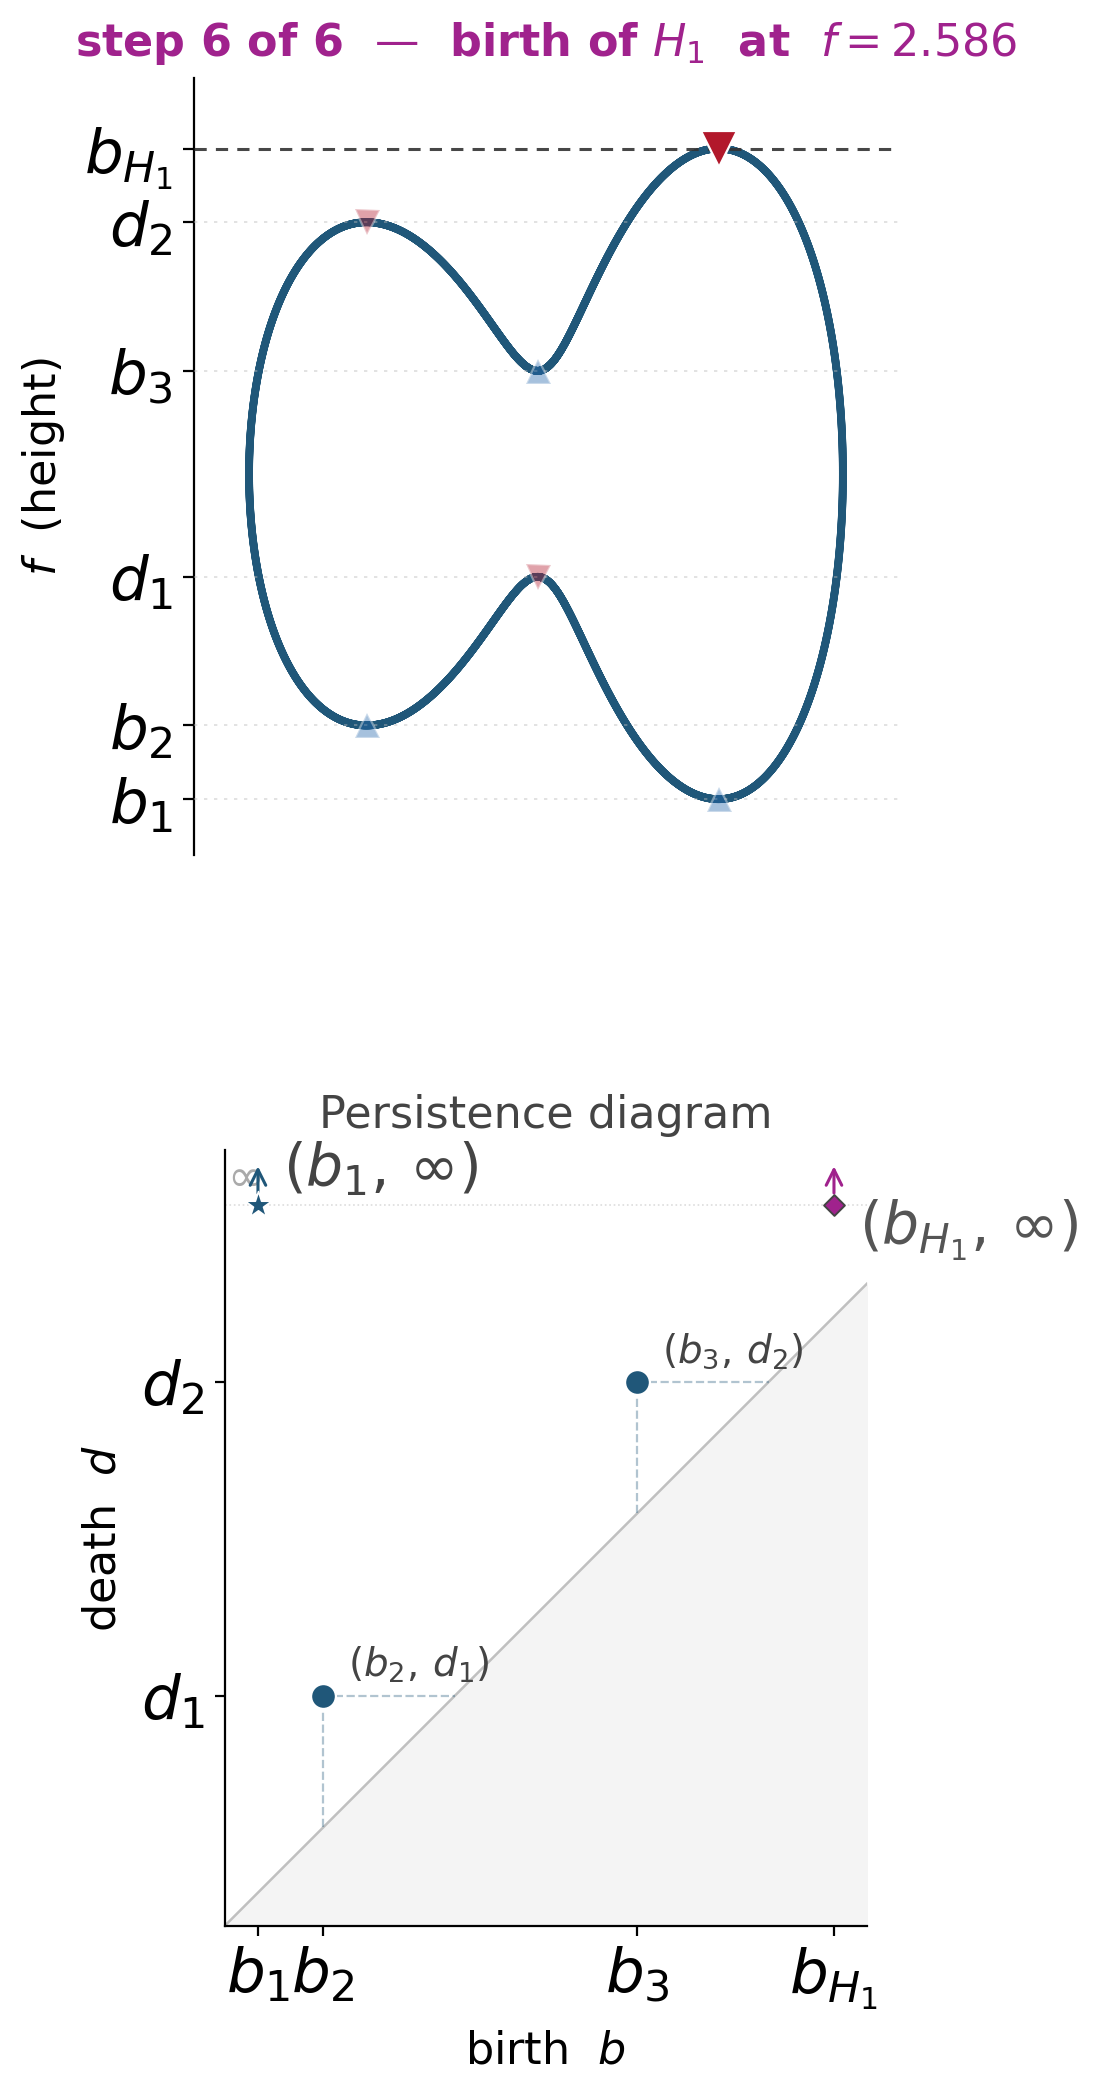
\includegraphics[height=0.8\textheight]{pd6.png}}
        \end{column}
    \end{columns}
\end{frame}

\begin{frame}{The Radial Persistence Transform}
    \begin{columns}[T]
        \begin{column}{0.45\textwidth}
            Fix a shape $\M\subset\R^2$ and a base point $x$.
            \begin{itemize}[<+->]
                \item Record the persistence diagram of the (squared Euclidean) distance
                      $\dist^2(\cdot,x)|_\M$.
                \item Sweep $x$ around a closed \textbf{observation loop}
                      $\gamma\colon\Sone\to\R^2$.
                \item Stacking the diagrams gives a \textbf{closed vineyard}
                      $\mathcal V(\M,\gamma)$; following one point gives a
                      \textbf{vine}.
            \end{itemize}
        \end{column}
        \begin{column}{0.55\textwidth}
            \centering
            \only<1>{%
                \begin{tikzpicture}
                    \node[anchor=south west,inner sep=0] (img) at (0,0)
                        {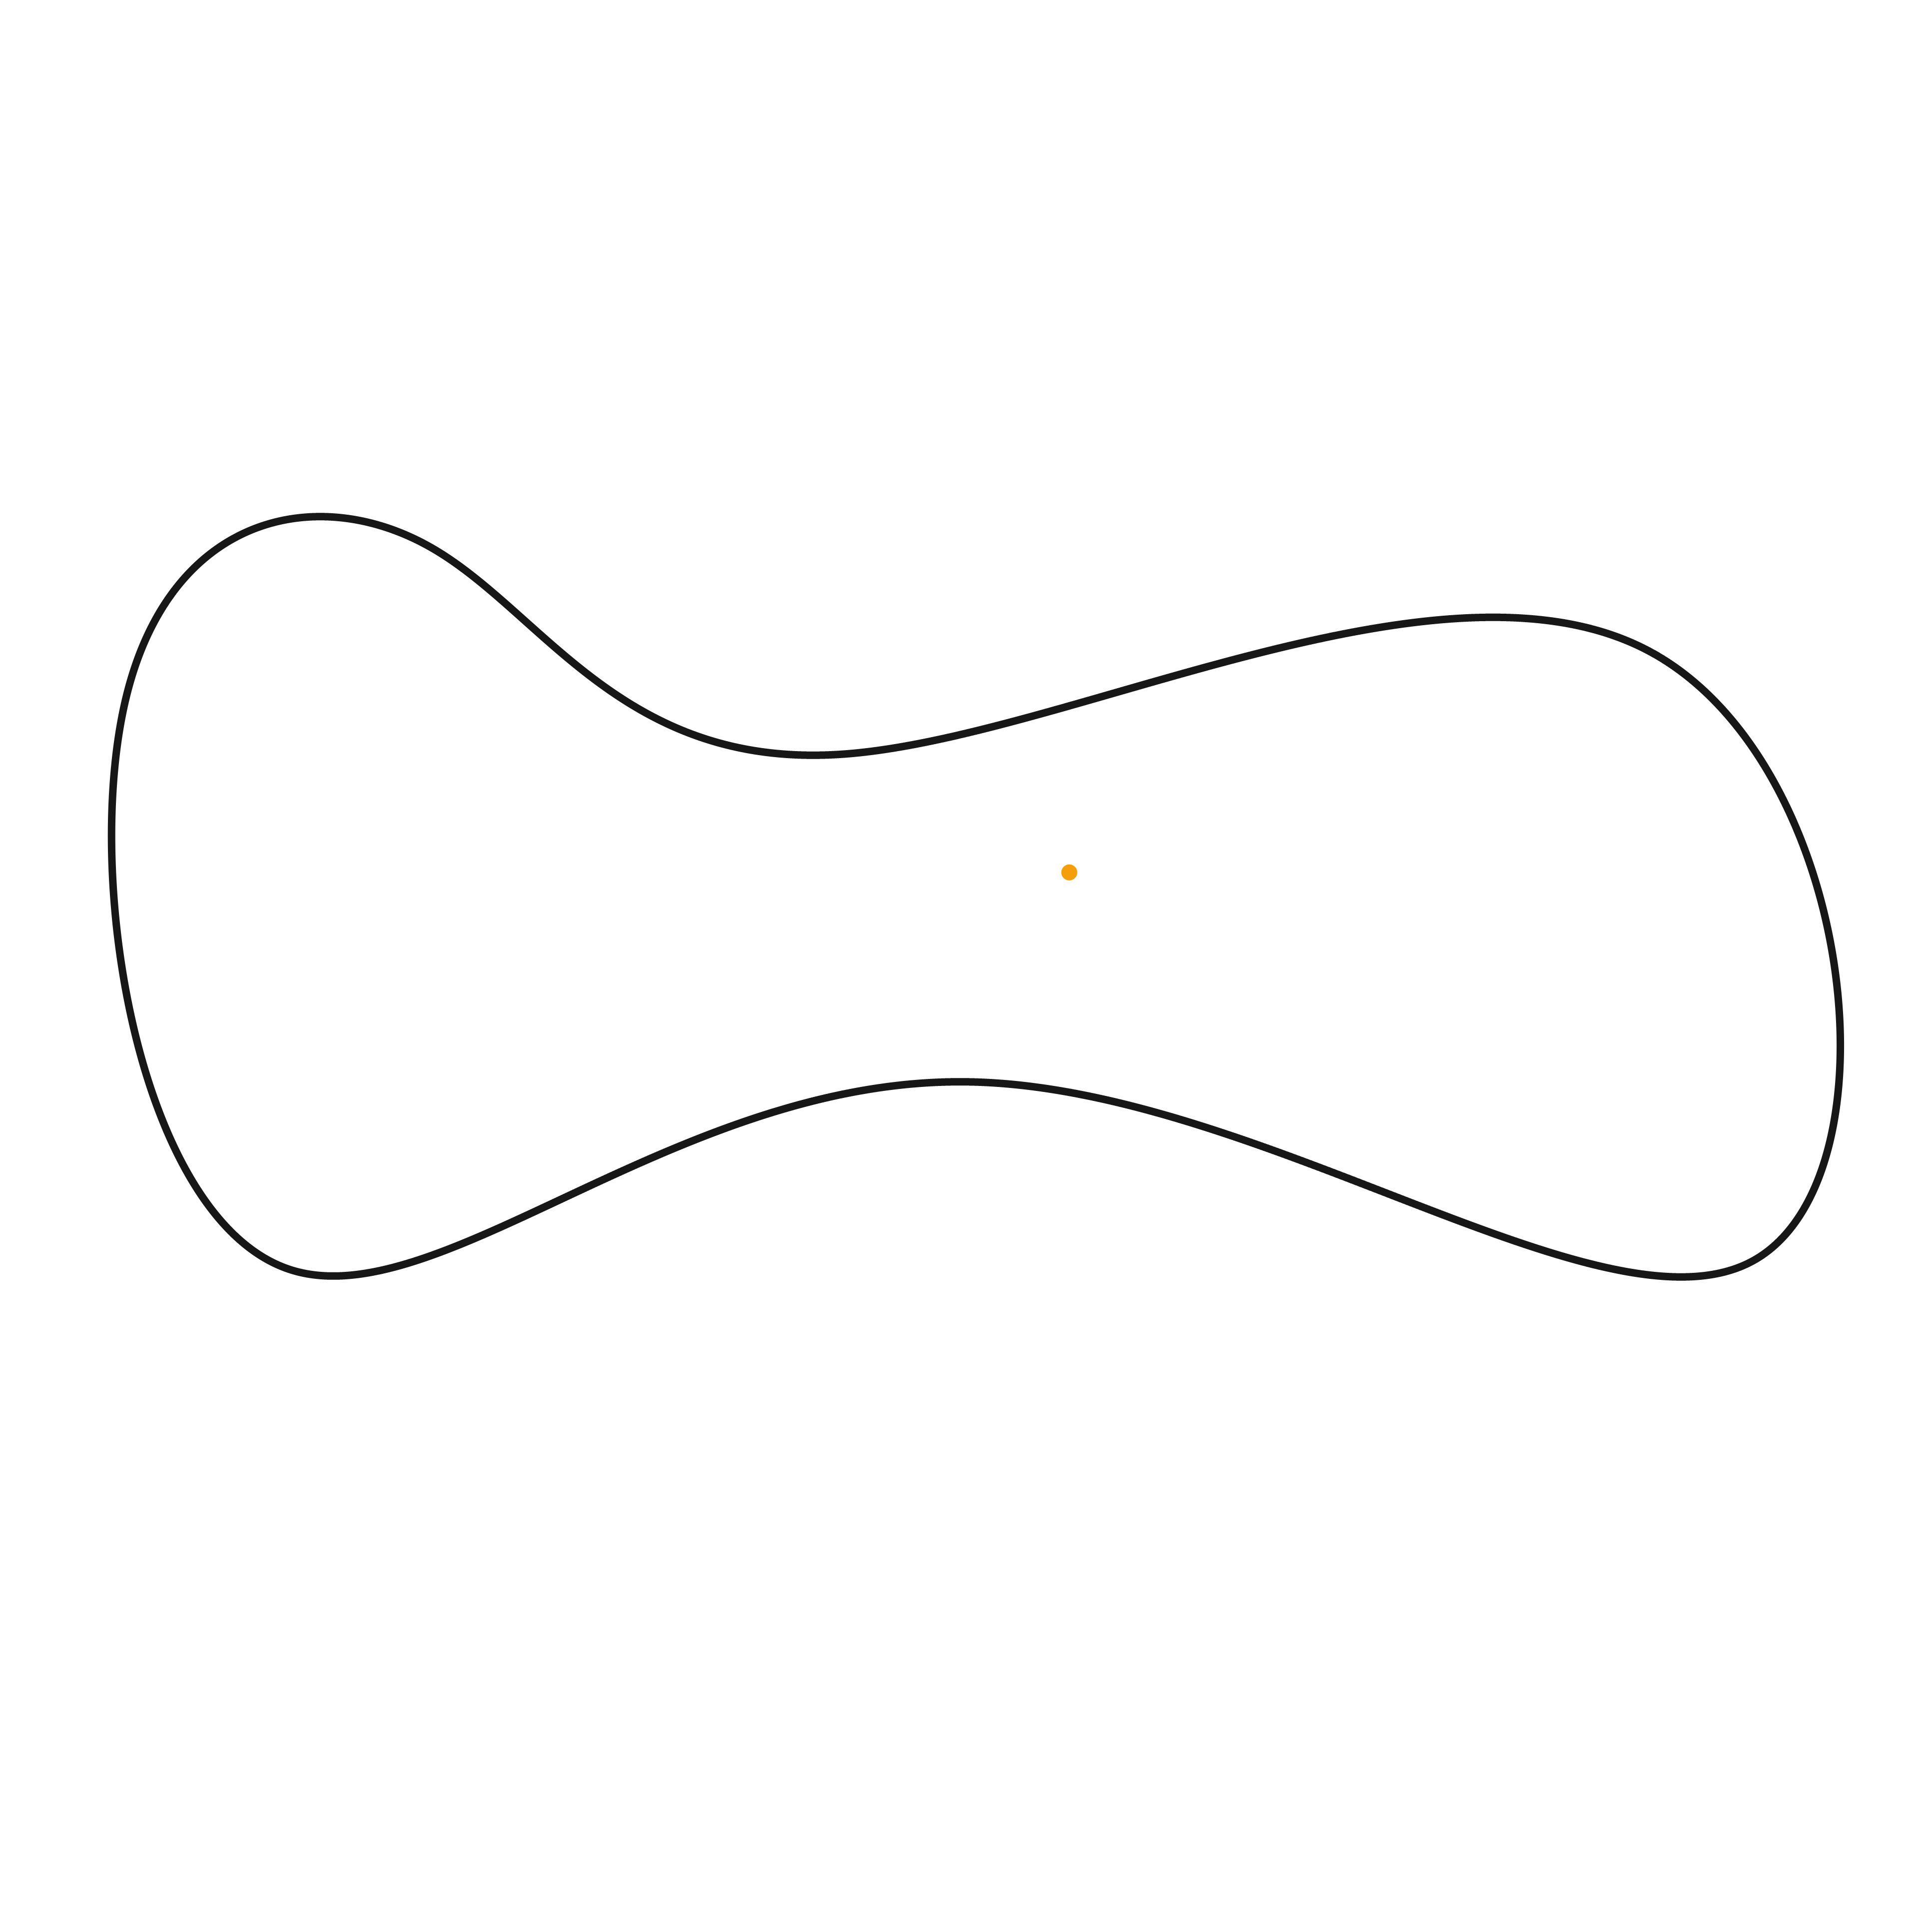
\includegraphics[width=0.8\linewidth]{slide_eg1.png}};
                    % coordinates below are fractions of the image: (0,0)=bottom-left, (1,1)=top-right
                    \begin{scope}[x={(img.south east)},y={(img.north west)}]
                        \definecolor{basepoint}{RGB}{245,158,11}
                        \fill[basepoint] (0.5533,0.5485) circle (0.009);
                        \draw[->,thick] (0.70,0.73) -- (0.569,0.568);
                        \node at (0.72,0.755) {$x$};
                    \end{scope}
                \end{tikzpicture}}
            \only<2>{%
                \begin{tikzpicture}
                    \node[anchor=south west,inner sep=0] (img) at (0,0)
                        {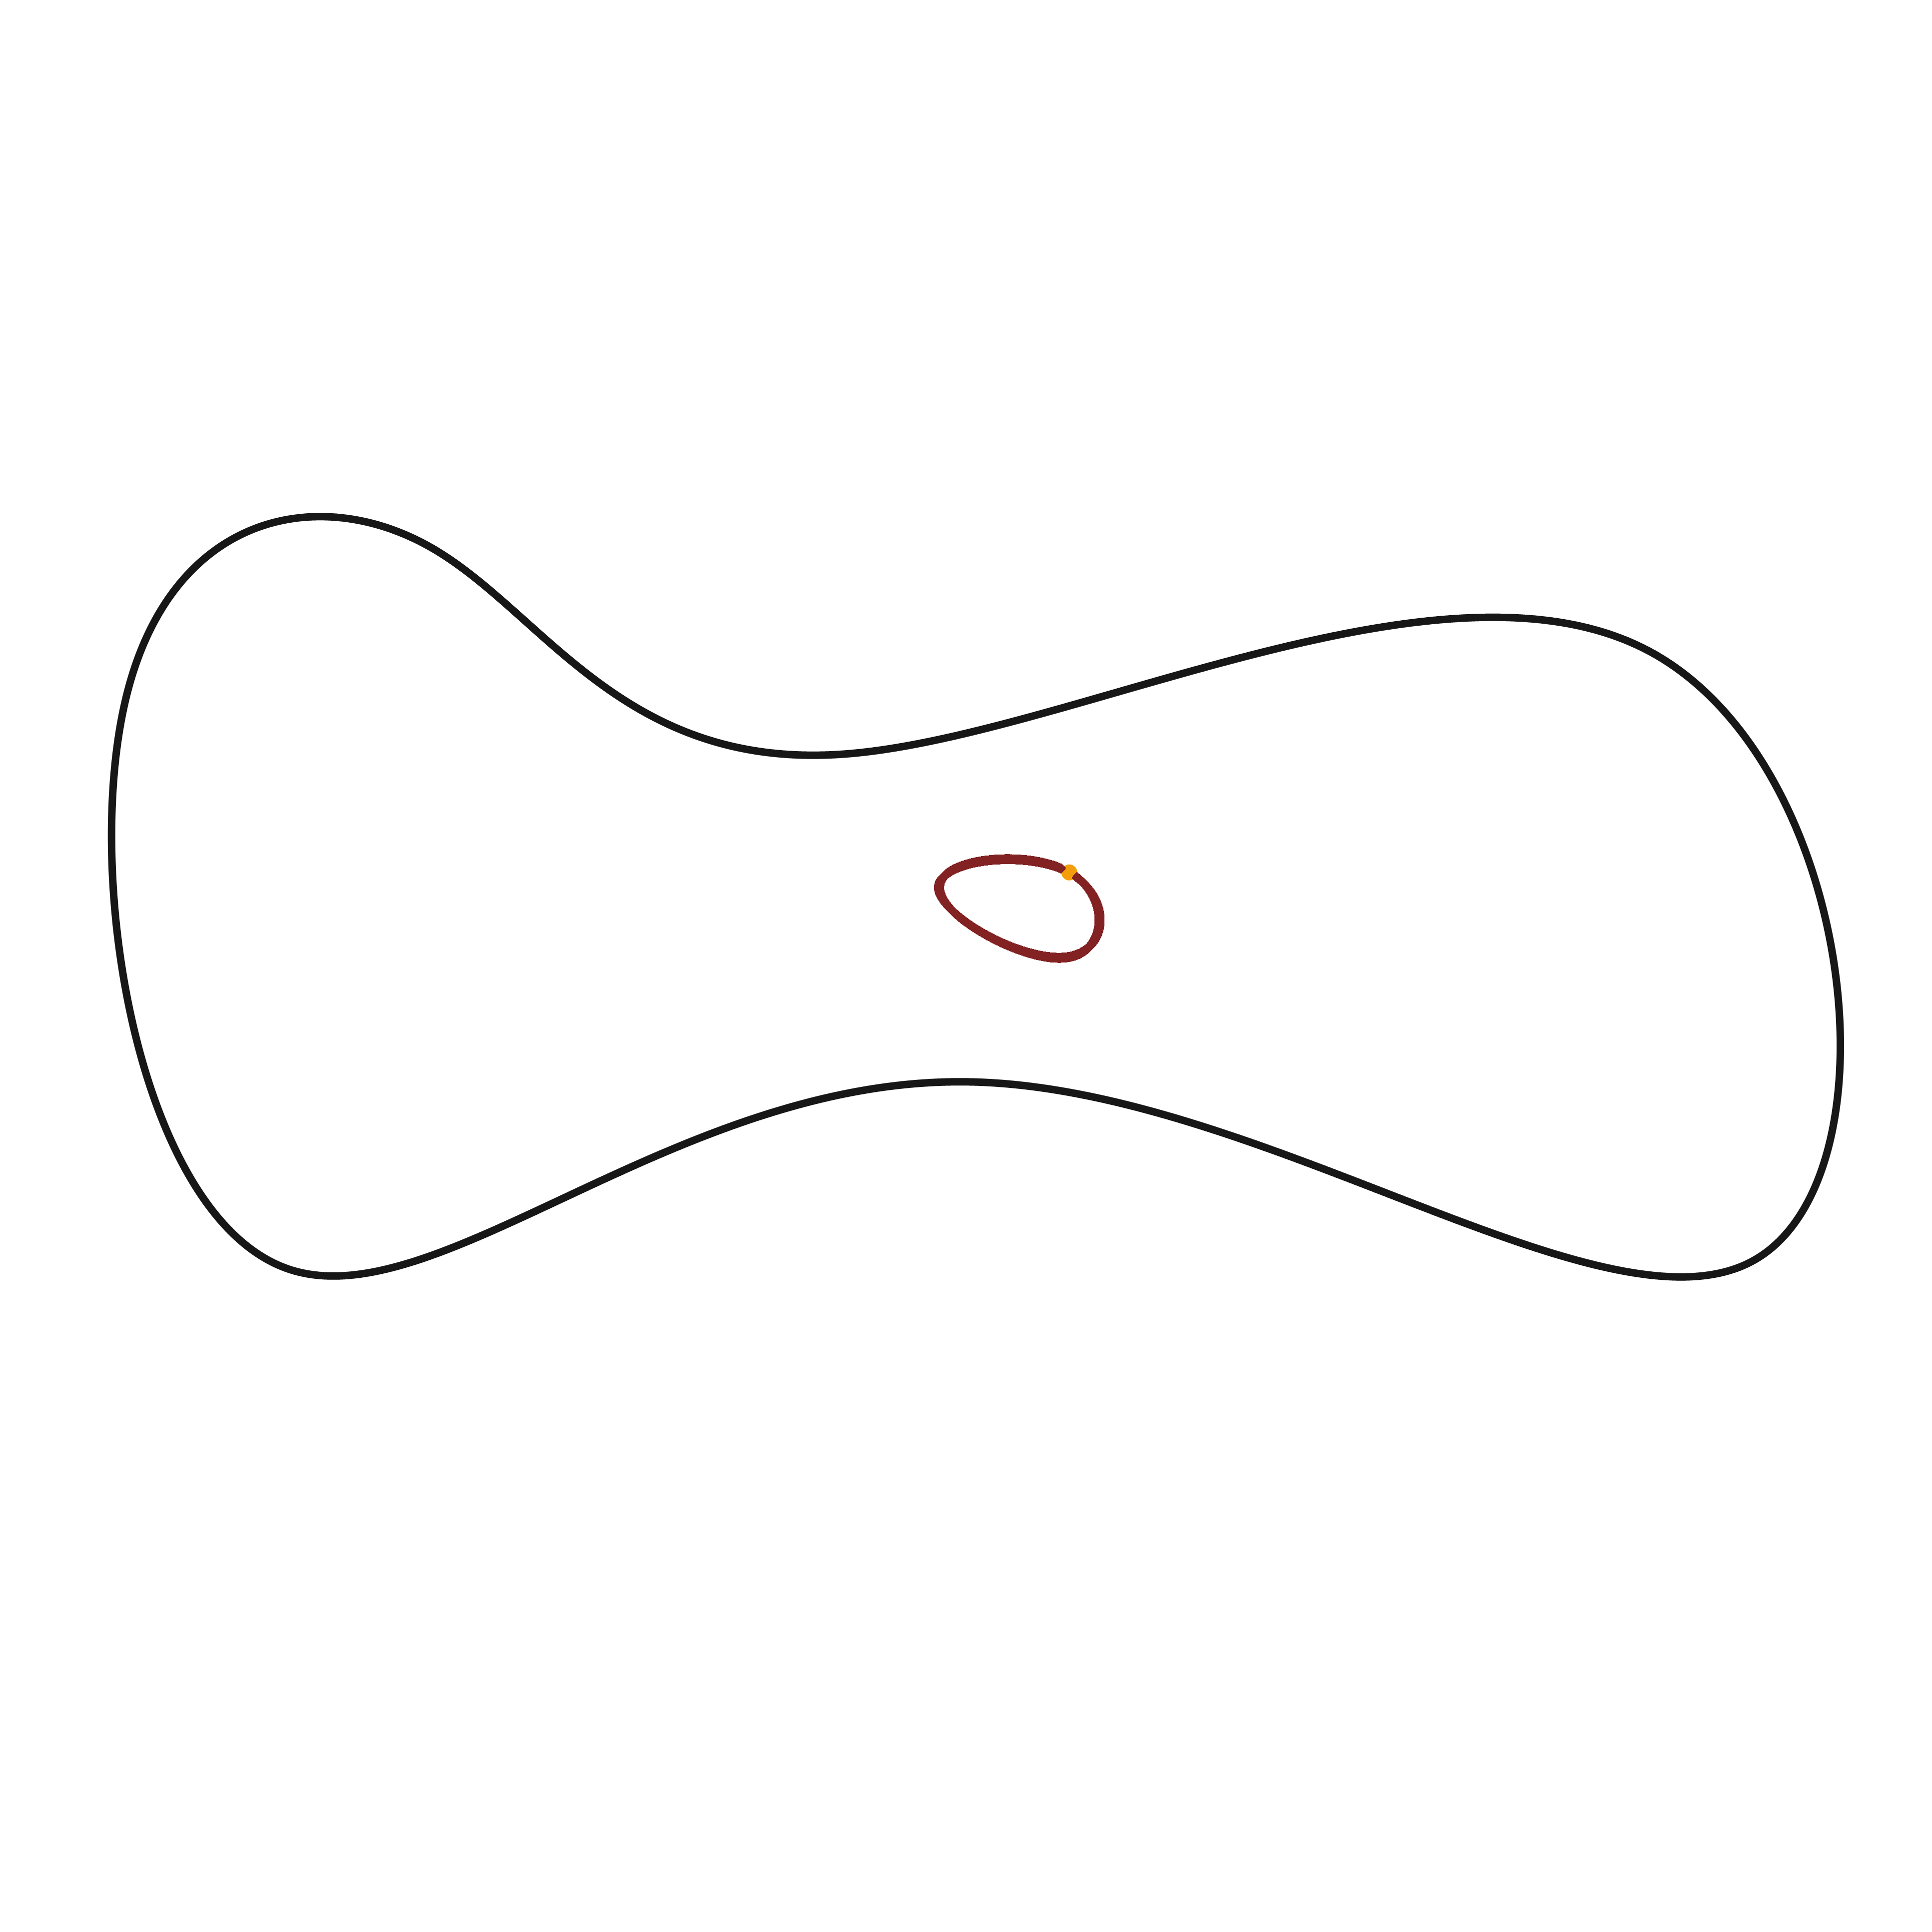
\includegraphics[width=0.8\linewidth]{slide_eg1loop_thick.png}};
                    % coordinates below are fractions of the image: (0,0)=bottom-left, (1,1)=top-right
                    \begin{scope}[x={(img.south east)},y={(img.north west)}]
                        \definecolor{basepoint}{RGB}{245,158,11}
                        \fill[basepoint] (0.5533,0.5485) circle (0.009);
                        \draw[->,thick] (0.70,0.73) -- (0.569,0.568);
                        \node at (0.72,0.755) {$x$};
                        \draw[->,thick] (0.45,0.395) -- (0.492,0.51);
                        \node at (0.435,0.365) {$\gamma$};
                    \end{scope}
                \end{tikzpicture}}
            \only<3>{%
                \vspace{-1.5em}
                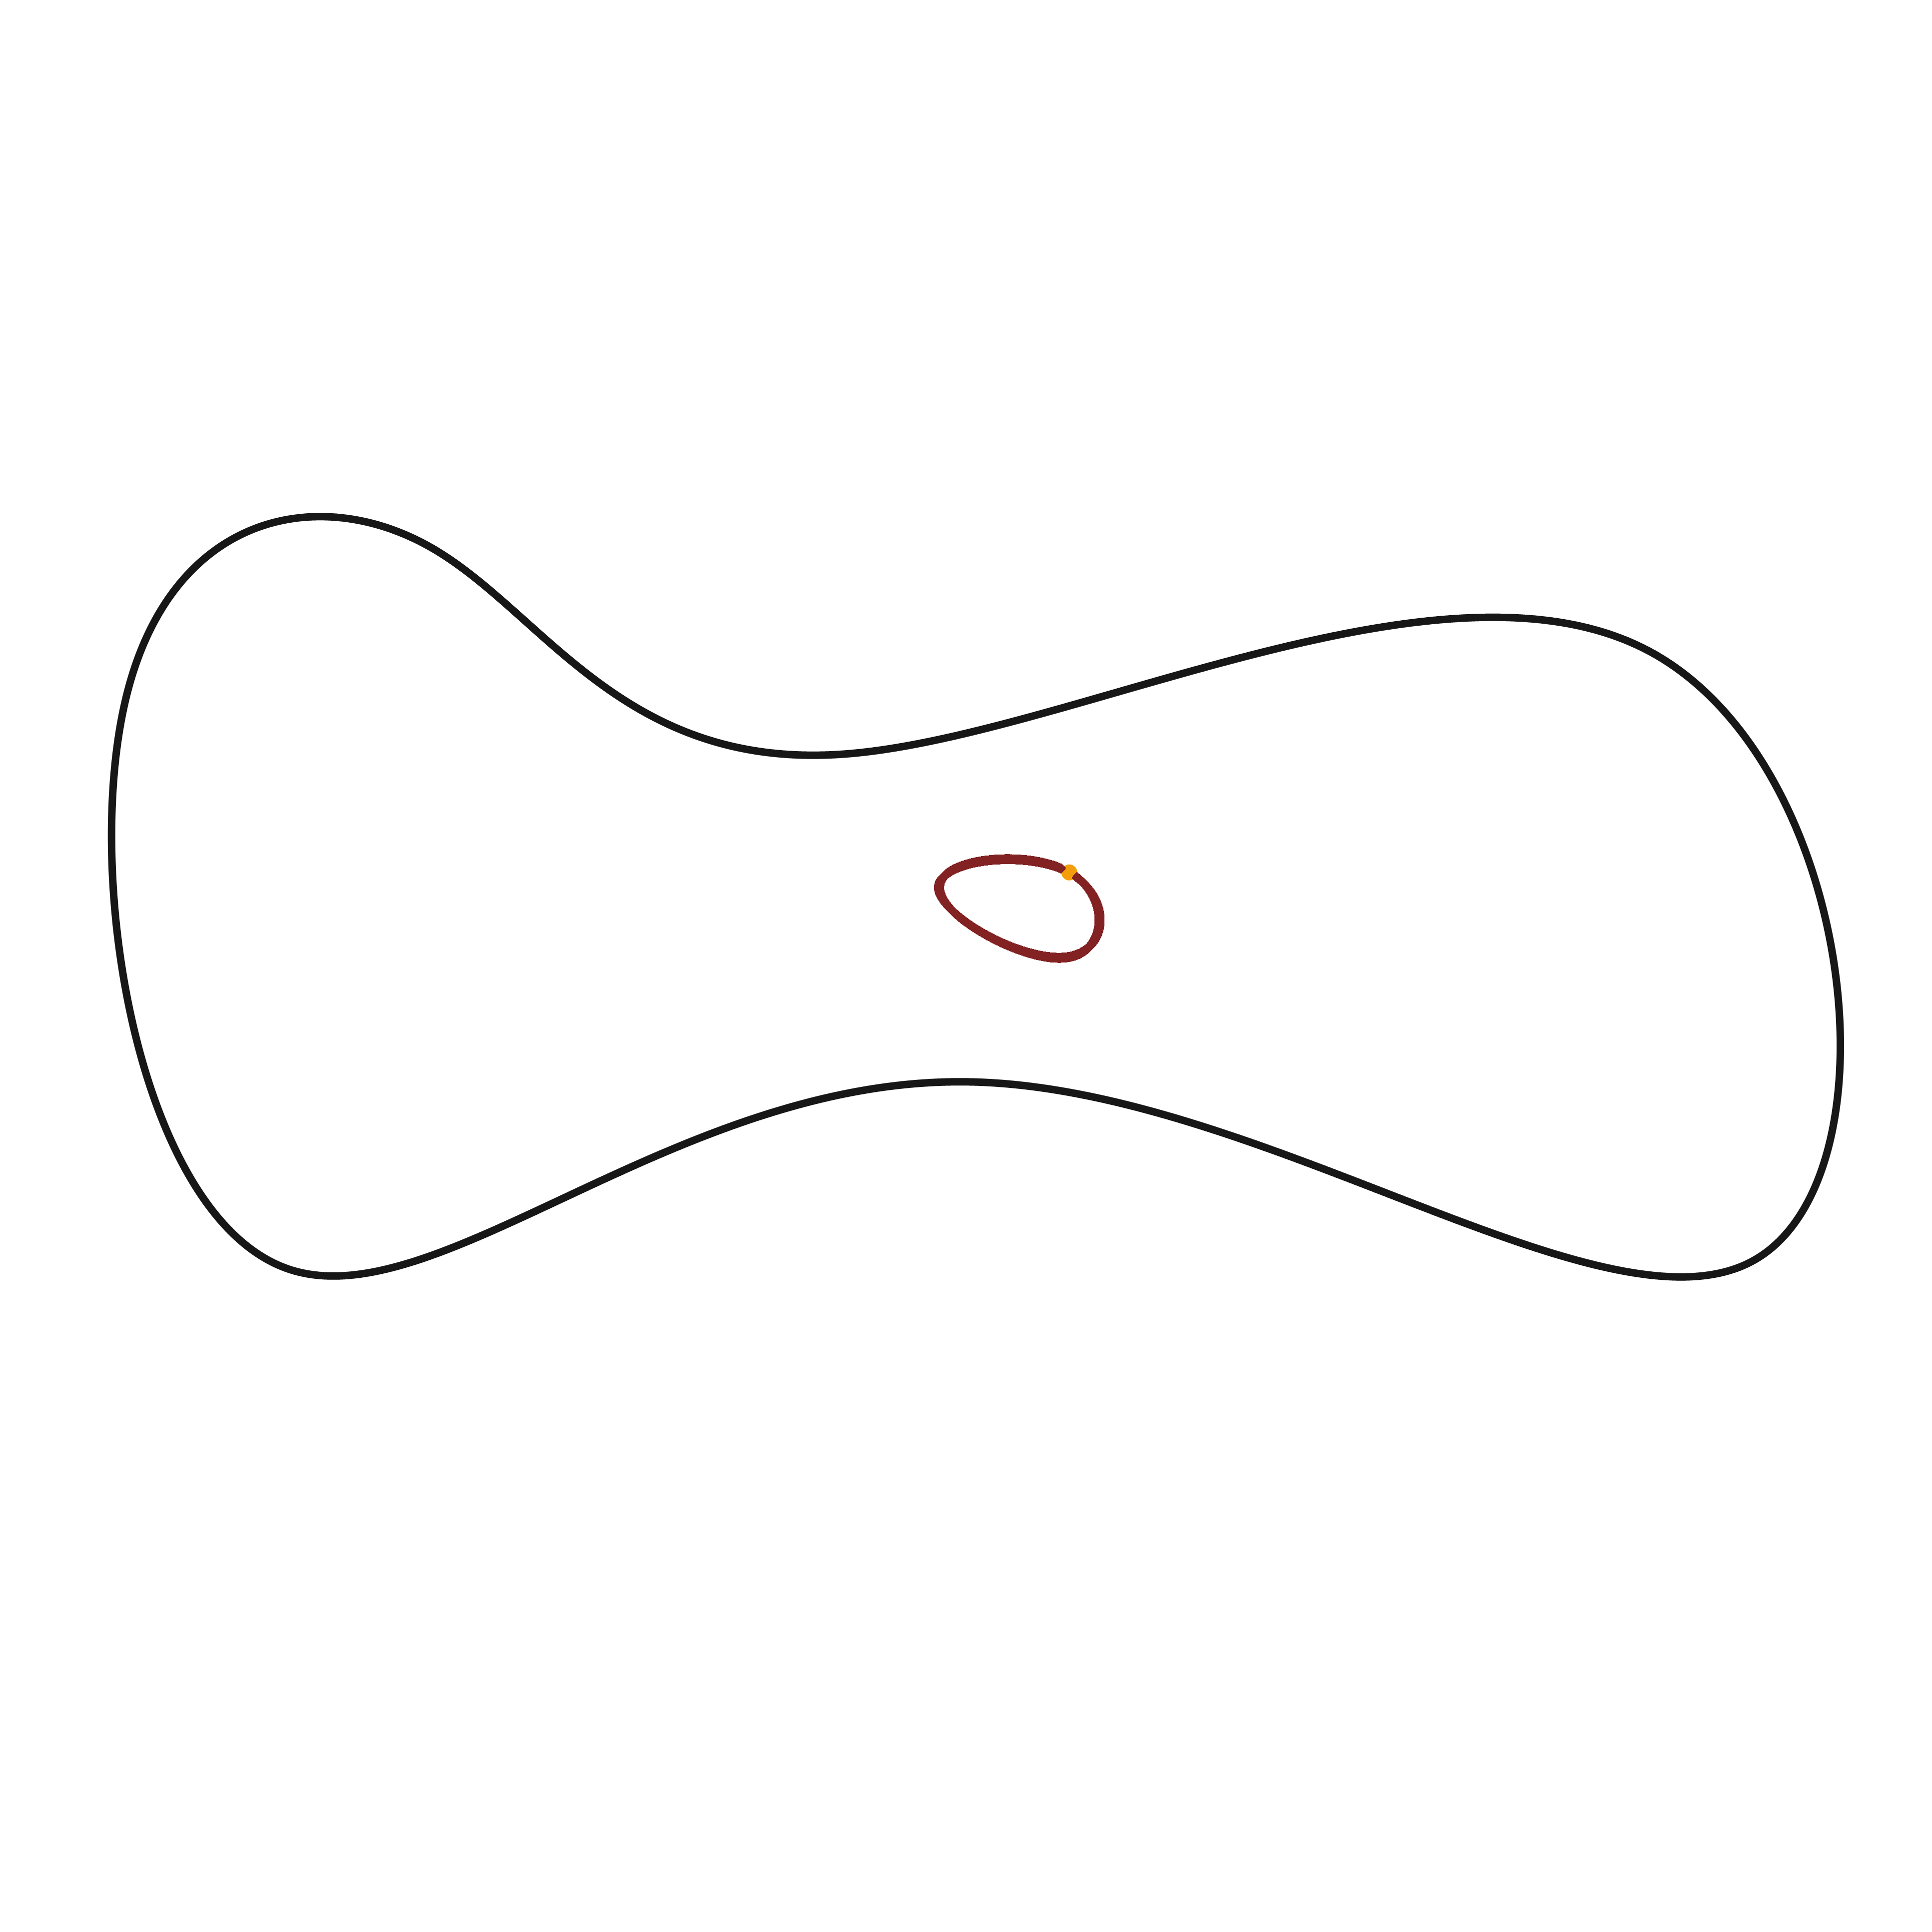
\includegraphics[width=0.455\linewidth]{slide_eg1loop_thick.png}\\
                \vspace{-2.1em}
                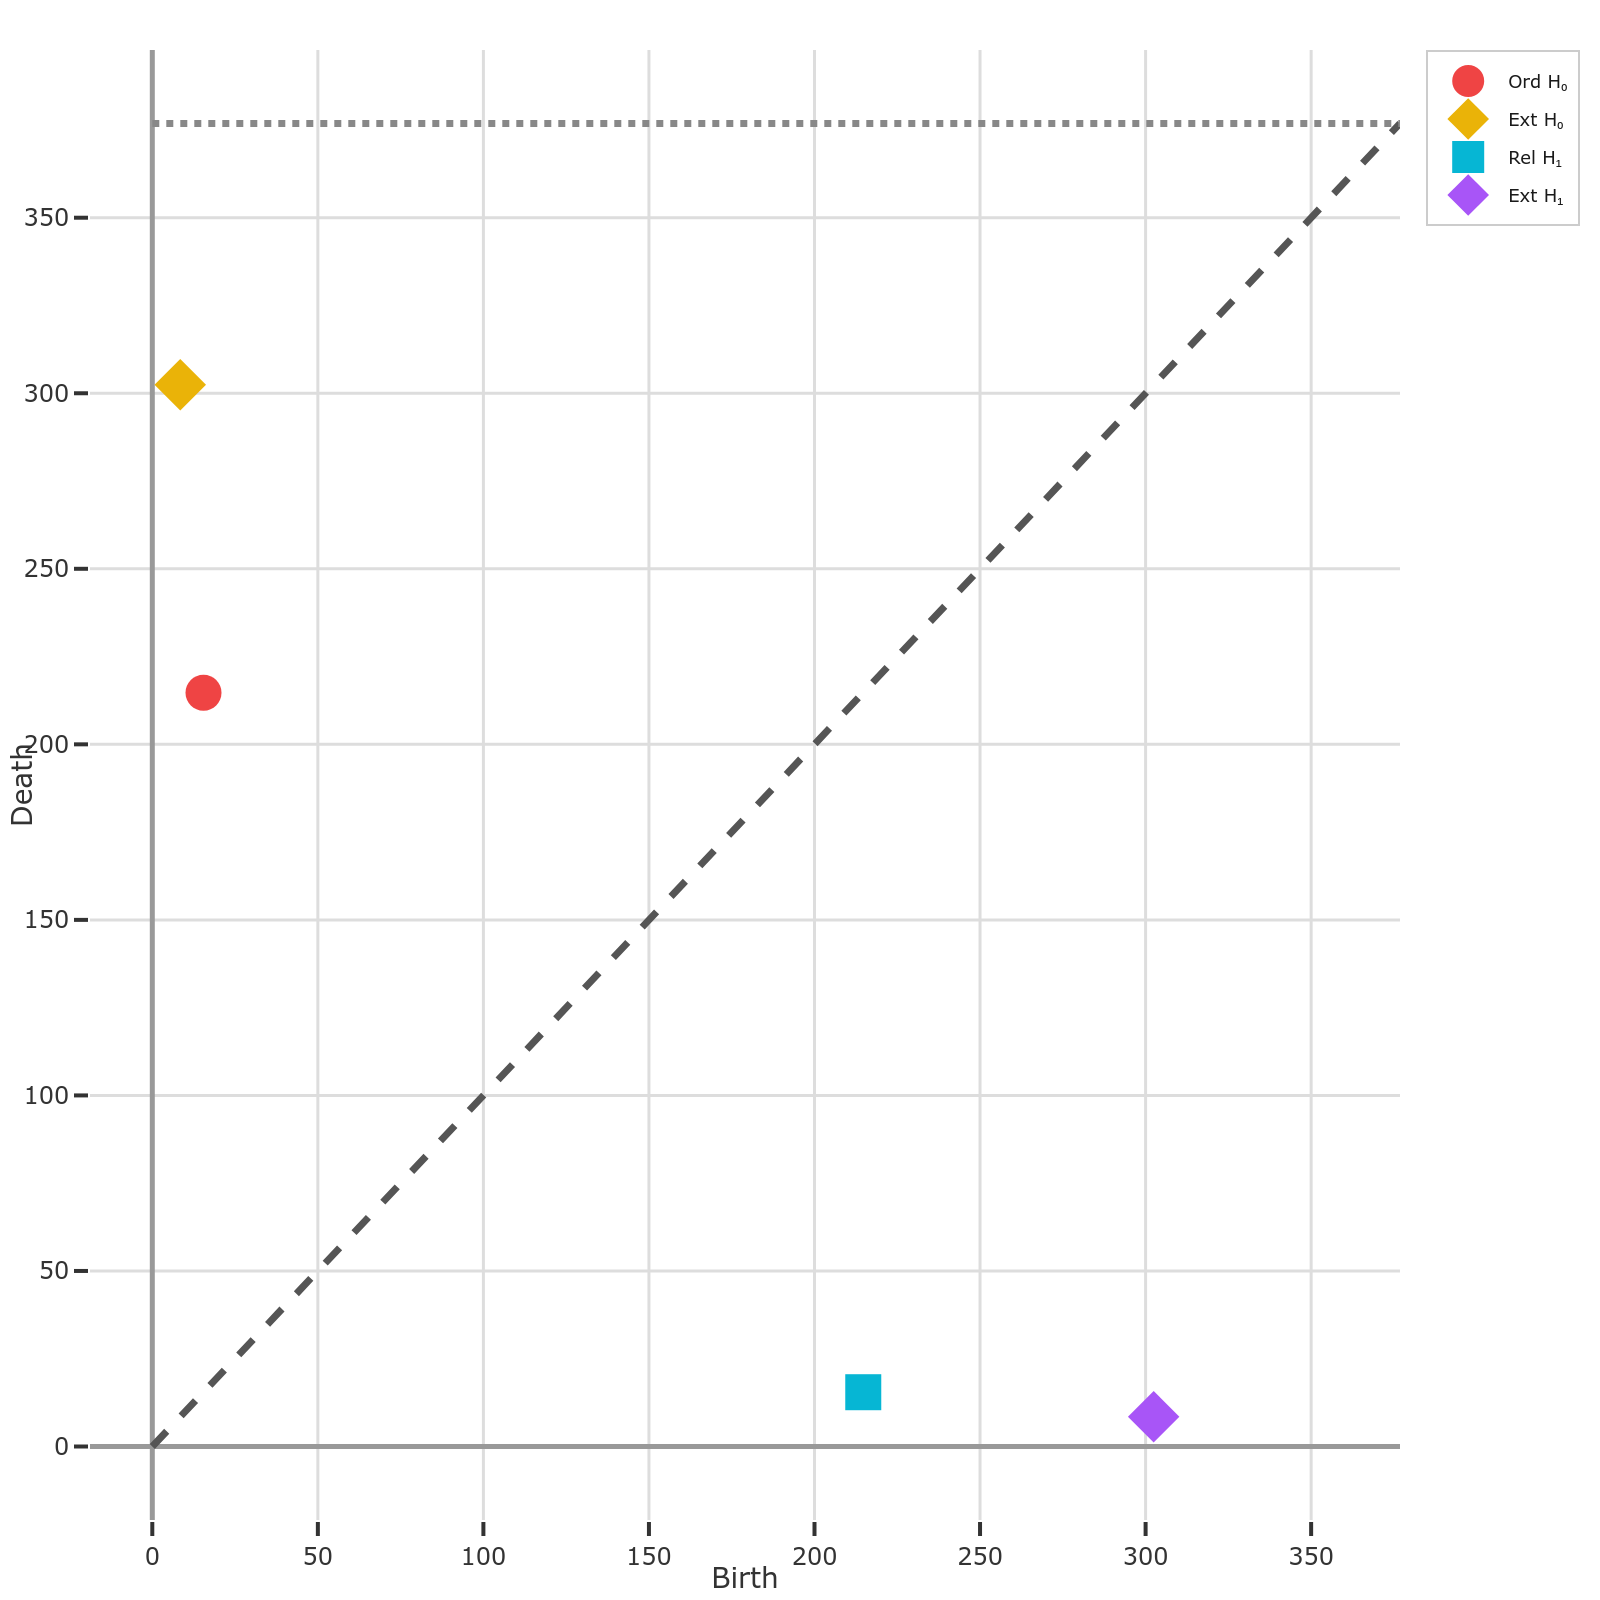
\includegraphics[width=0.455\linewidth]{slide_eg1pd.png}
                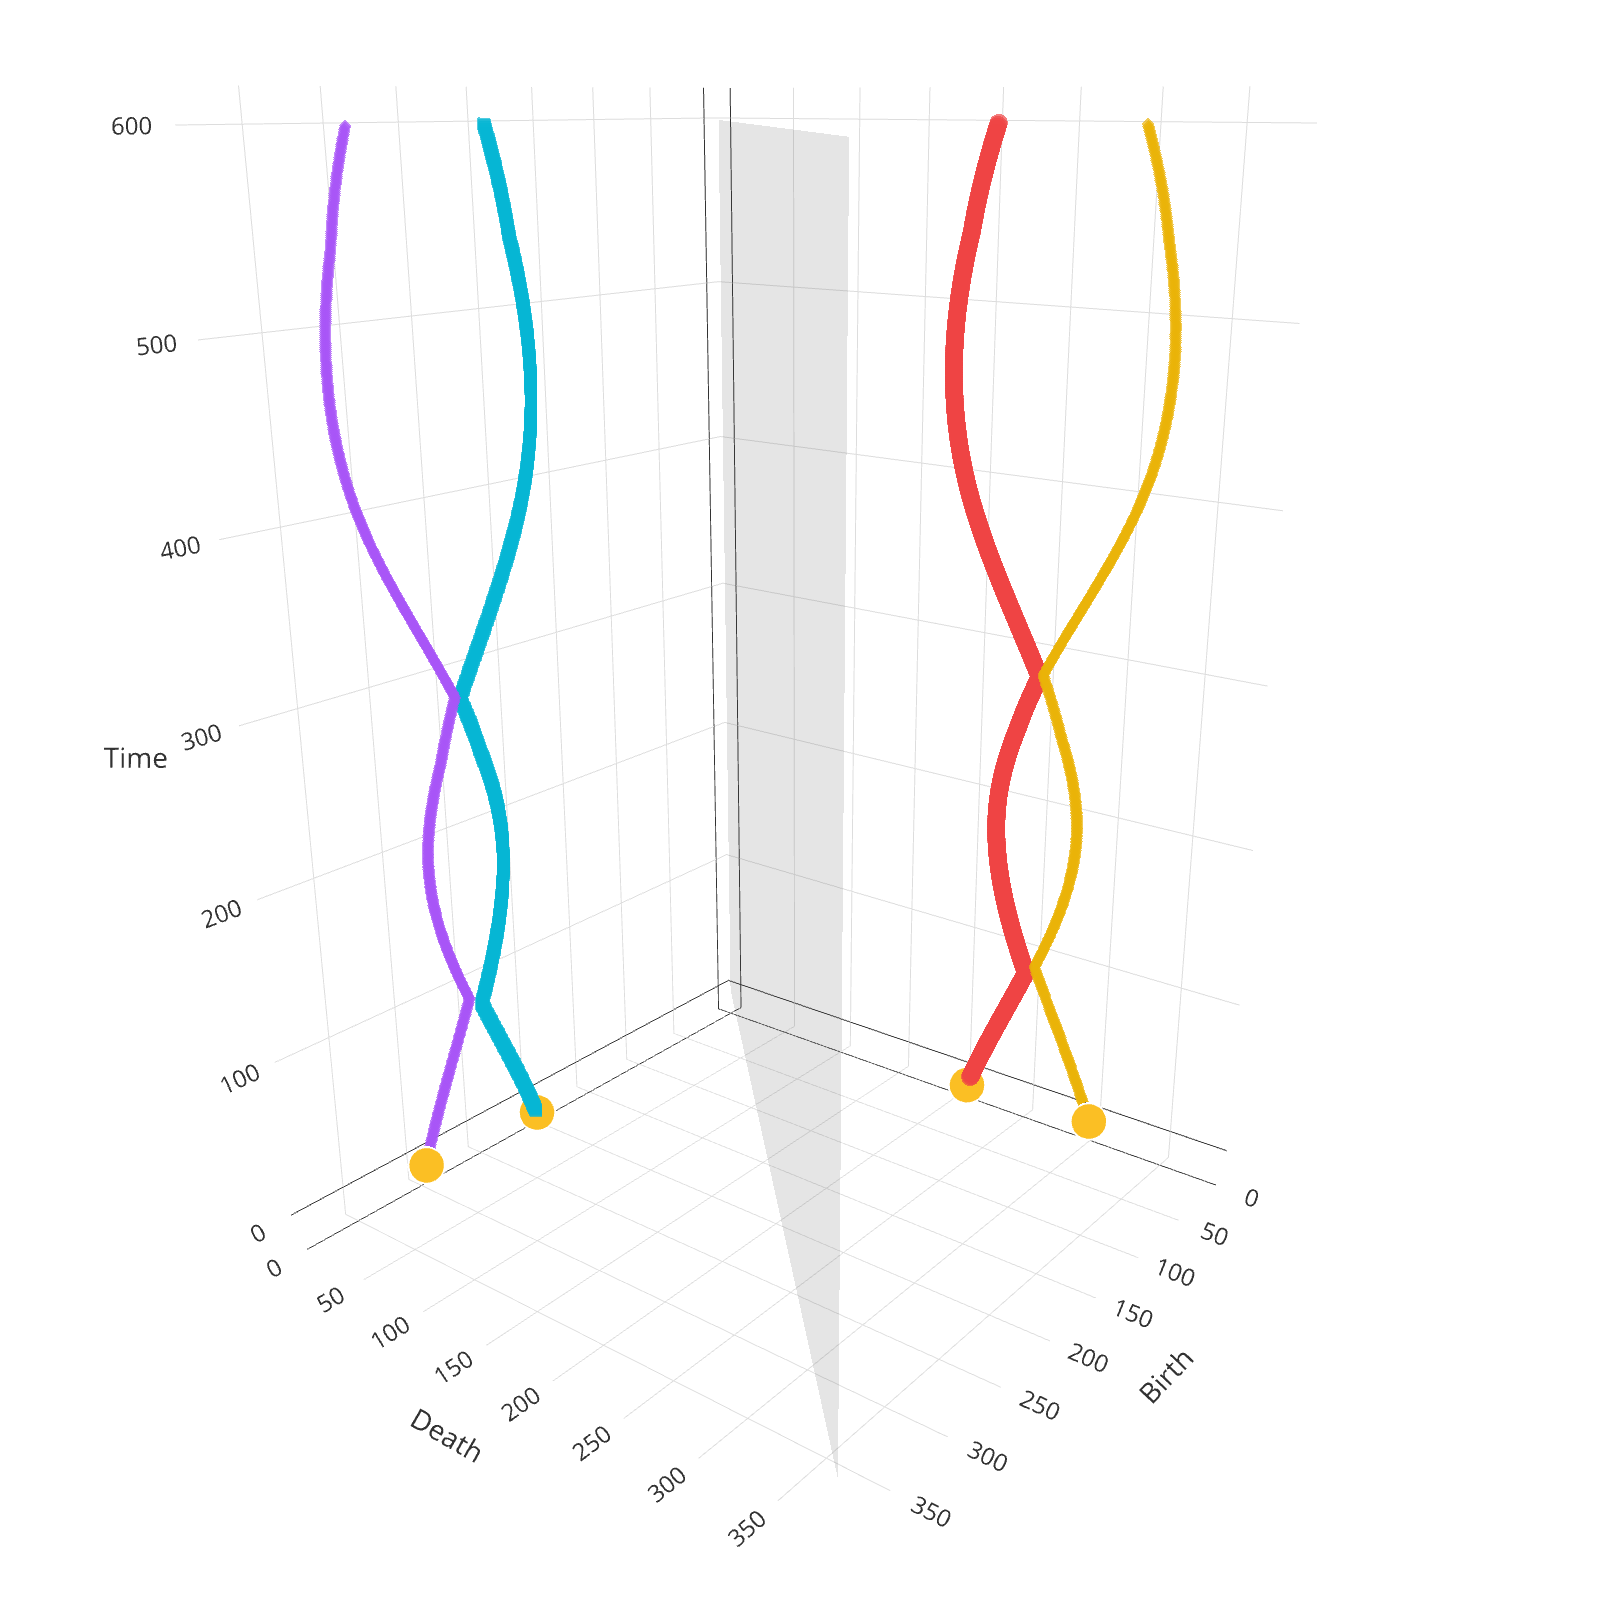
\includegraphics[width=0.455\linewidth]{slide_eg1vine.png}}
            % {\scriptsize Symmetry set (blue), focal set (purple), vineyard along the loop.}
        \end{column}
    \end{columns}
    % \note{Plain-language setup: distance-to-a-moving-point, read topologically.
    % The loop must be closed so monodromy is defined. ~1.5 min.}
\end{frame}

\begin{frame}{Monodromy in Vineyards}
            % \item \textbf{Persistence diagram:} birth--death pairs $(b,d)$ of features
        %       of the sublevel sets of $f$.
        % \item \textbf{Vineyard:} stability $\Rightarrow$ points move continuously
        %       as $\gamma(t)$ varies $\Rightarrow$ vines.
    \textbf{Monodromy of order $k$:} after $k$ traversals of the loop every vine returns to itself --- the vines \textbf{braid}, and can even knot.
    % \end{itemize}
    \vspace{-0.8em}
    \begin{figure}[h!]
    \centering
    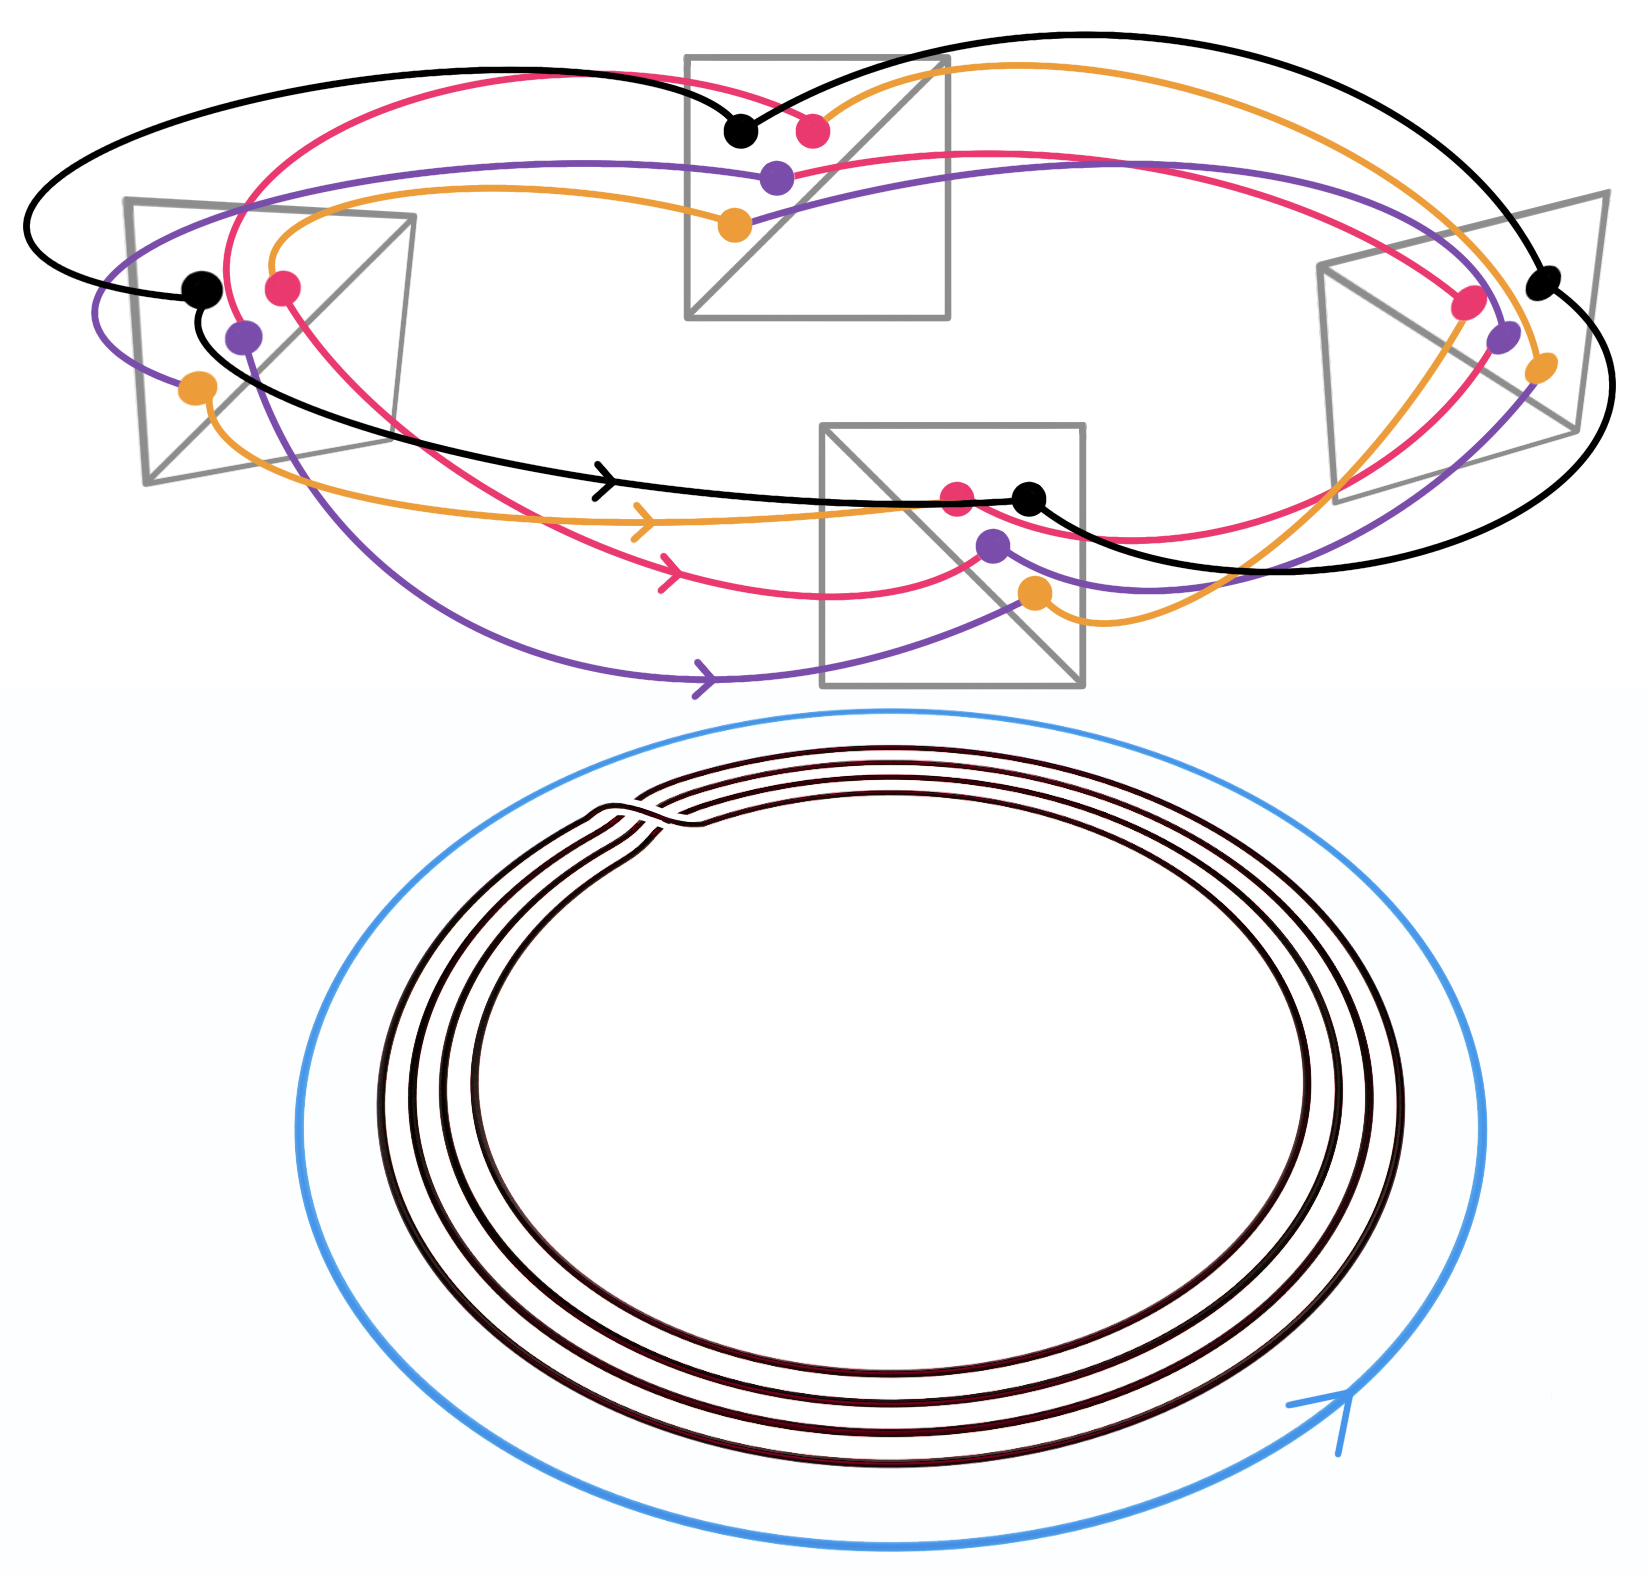
\includegraphics[width=0.365\linewidth]{sketch_2_with_link_again.png}
    \end{figure}
    % \vspace{0.3em}
    % \begin{block}{Why care?}
    %     Monodromy obstructs feature tracking and complicates downstream TDA
    %     analysis. Until recently, almost nothing was known about \emph{which
    %     geometry forces it}.
    % \end{block}
    \vspace{-1.5em}
    \braidcite
\end{frame}

\begin{frame}{The driving question}
    \begin{center}
        {\Large Which geometric features of a shape \\[4pt]
        \textbf{force} monodromy in its vineyard?}
    \end{center}
    \vspace{1em}
    \begin{itemize}
        \item Answer lives in the \textbf{singularity theory of the distance
              function}.
        \item Two classical objects: the \textbf{symmetry set} and the
              \textbf{focal set}.
        \item Geometry of these sets
              $\;\longleftrightarrow\;$ topology of the vineyard.
    \end{itemize}
    \note{The thesis question. Keep crisp; the ``how'' is next. ~1 min.}
\end{frame}

%========================================================================
\section{The theory}
%========================================================================

\begin{frame}{Symmetry set, focal set, generalized symmetry set}
    \begin{columns}[T]
        \begin{column}{0.50\textwidth}
            \begin{itemize}
                \item \textbf{Focal set} $\foc(\M)$ (evolute): centres of
                      curvature --- degenerate critical points of the distance.
                \item \textbf{Symmetry set} $\sym(\M)$: centres of circles tangent
                      to $\M$ in $\ge 2$ places.
                \item \textbf{Generalized symmetry set}
                      $\gsym(\M)=\sym(\M)\cup\foc(\M)$ also called as the \textbf{bifurcation set.}
            \end{itemize}
            \vspace{0.3em}
            % {\footnotesize Generic planar singularities are classified (Arnold;Bruce--Giblin--Gibson).}
        \end{column}
        \begin{column}{0.50\textwidth}
            \centering
            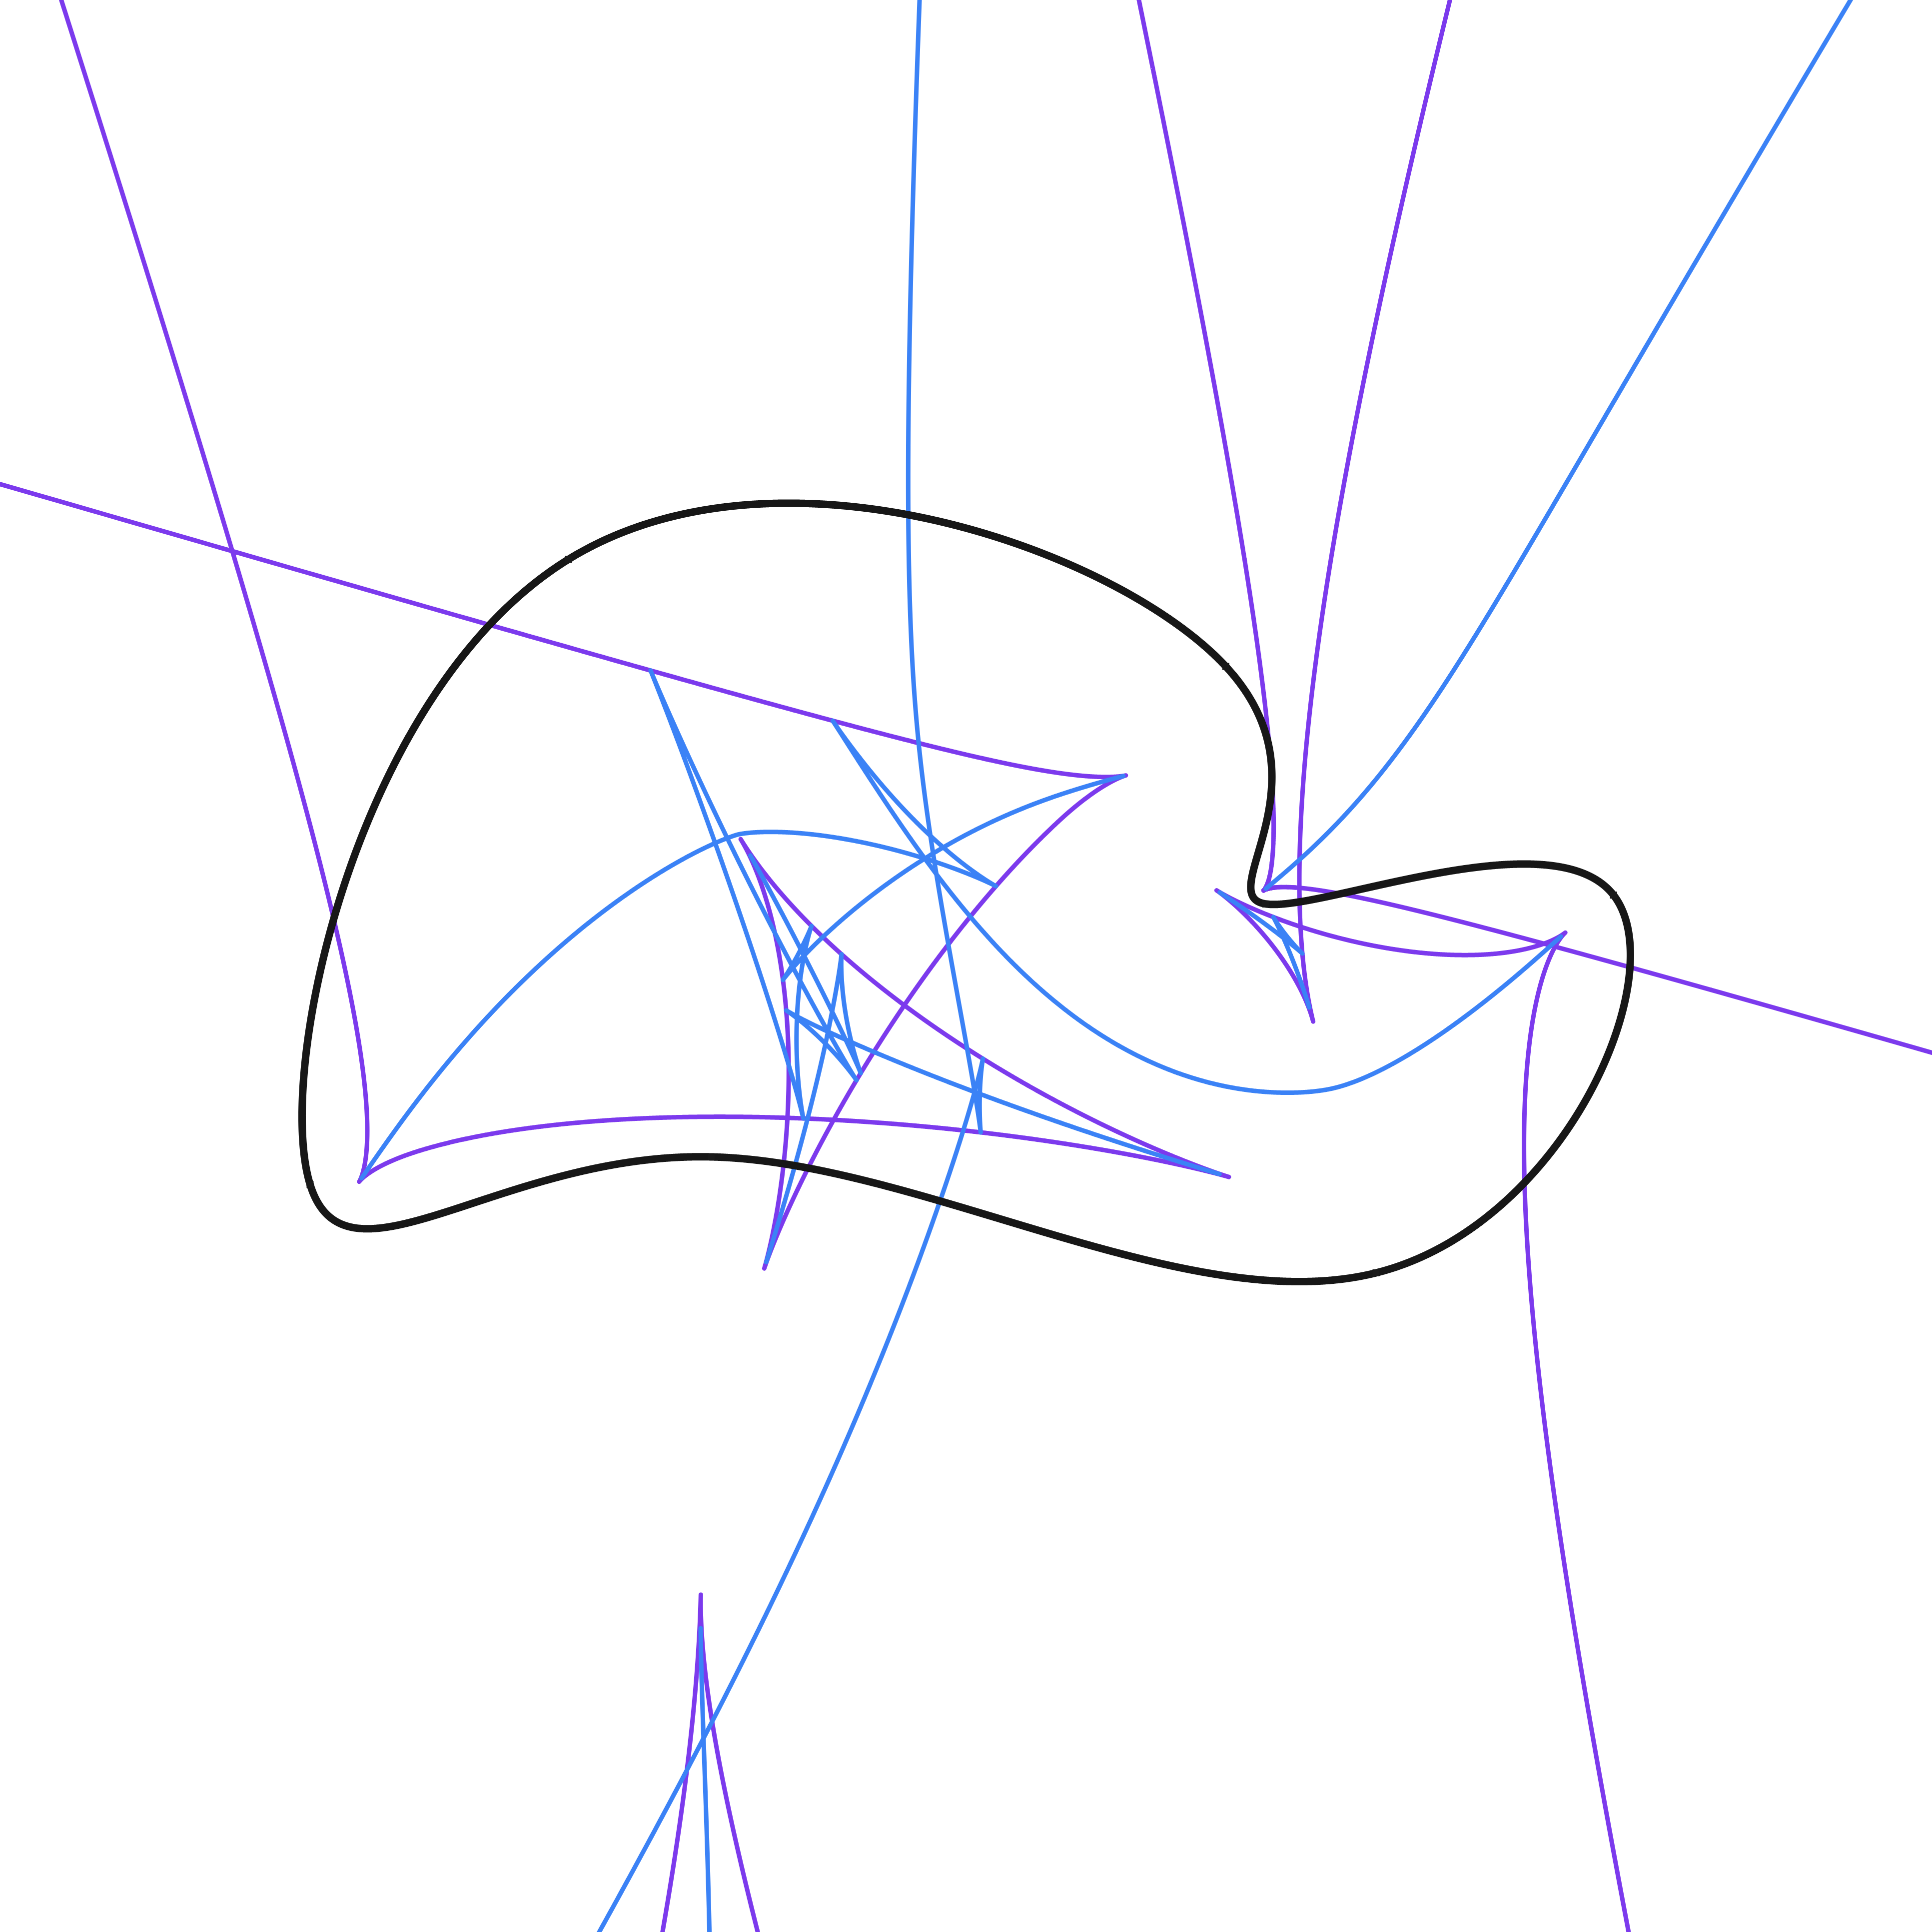
\includegraphics[width=0.8\linewidth]{slide_eg2.png}\\
            % {\scriptsize The generic planar singularities.}
        \end{column}
    \end{columns}
    \note{Give the map, not the proofs. ~2 min.}
\end{frame}

\begin{frame}{Generic planar singularities}
    They are classified according to Arnold; Bruce--Giblin--Gibson.
    \begin{figure}
        \centering
        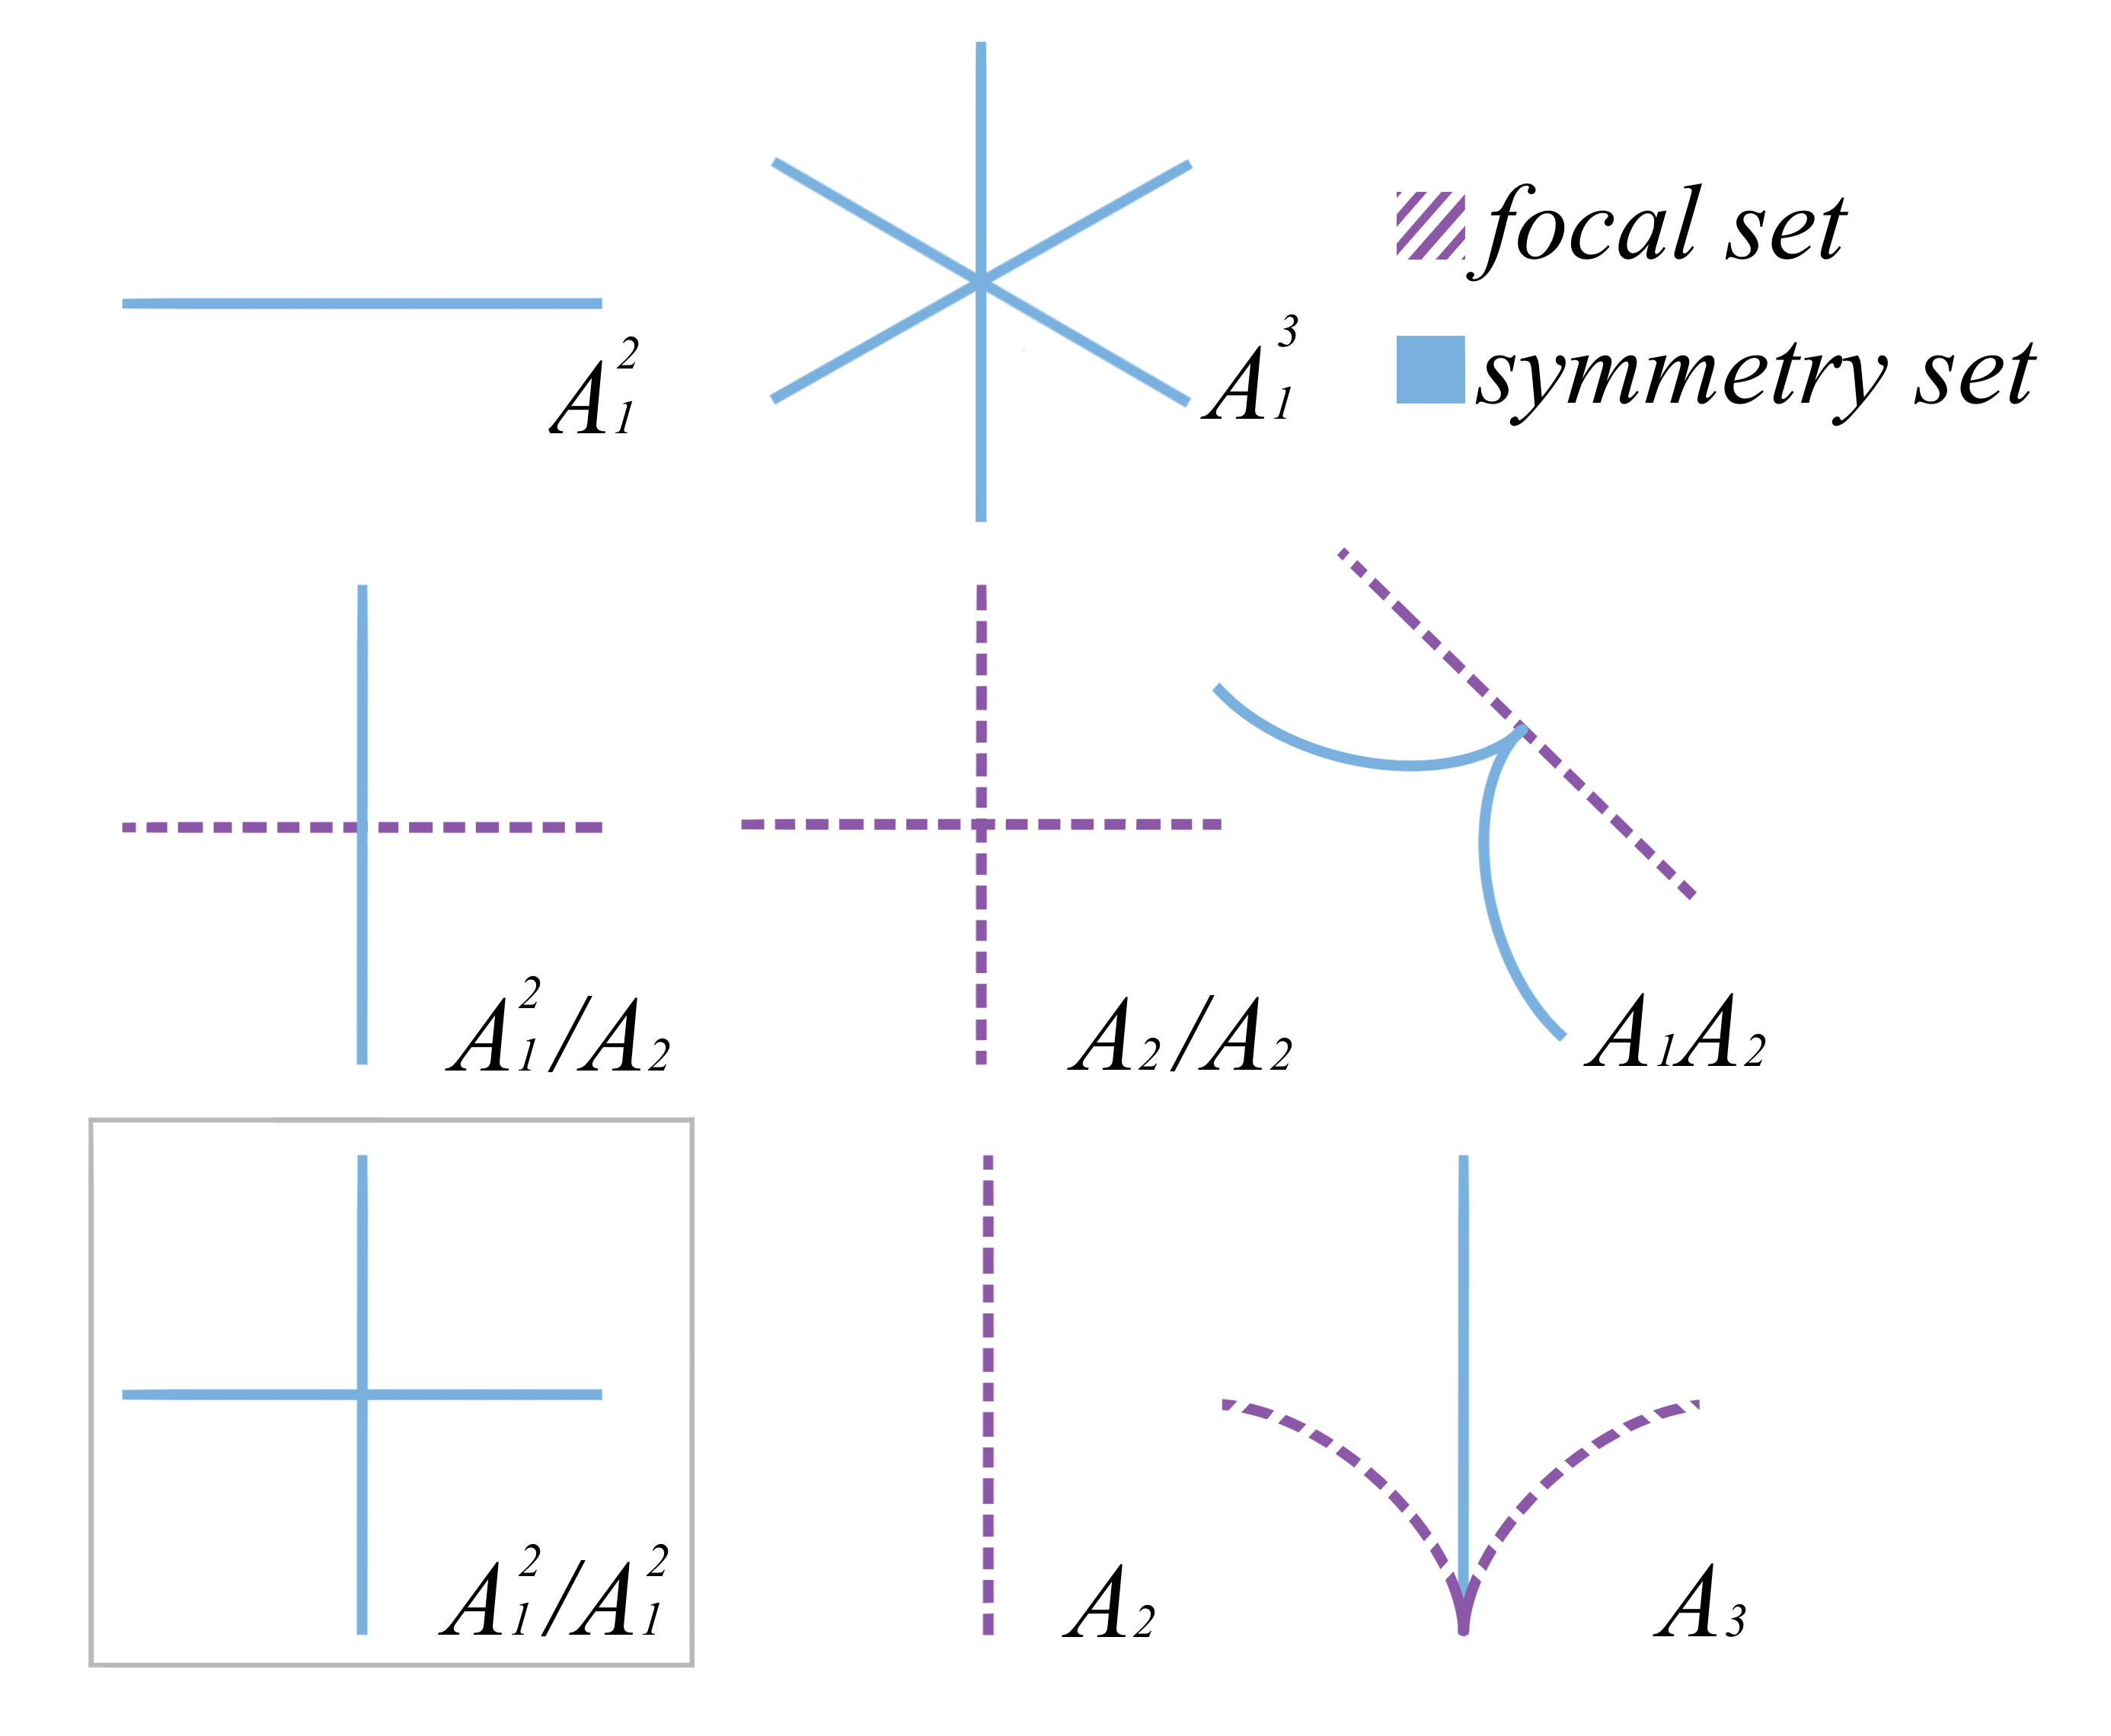
\includegraphics[width=0.5\linewidth]{symmetry_focal_corrected_2.png}
    \end{figure}
\end{frame}

\begin{frame}{Generic planar singularities}
    \begin{figure}
        \centering
        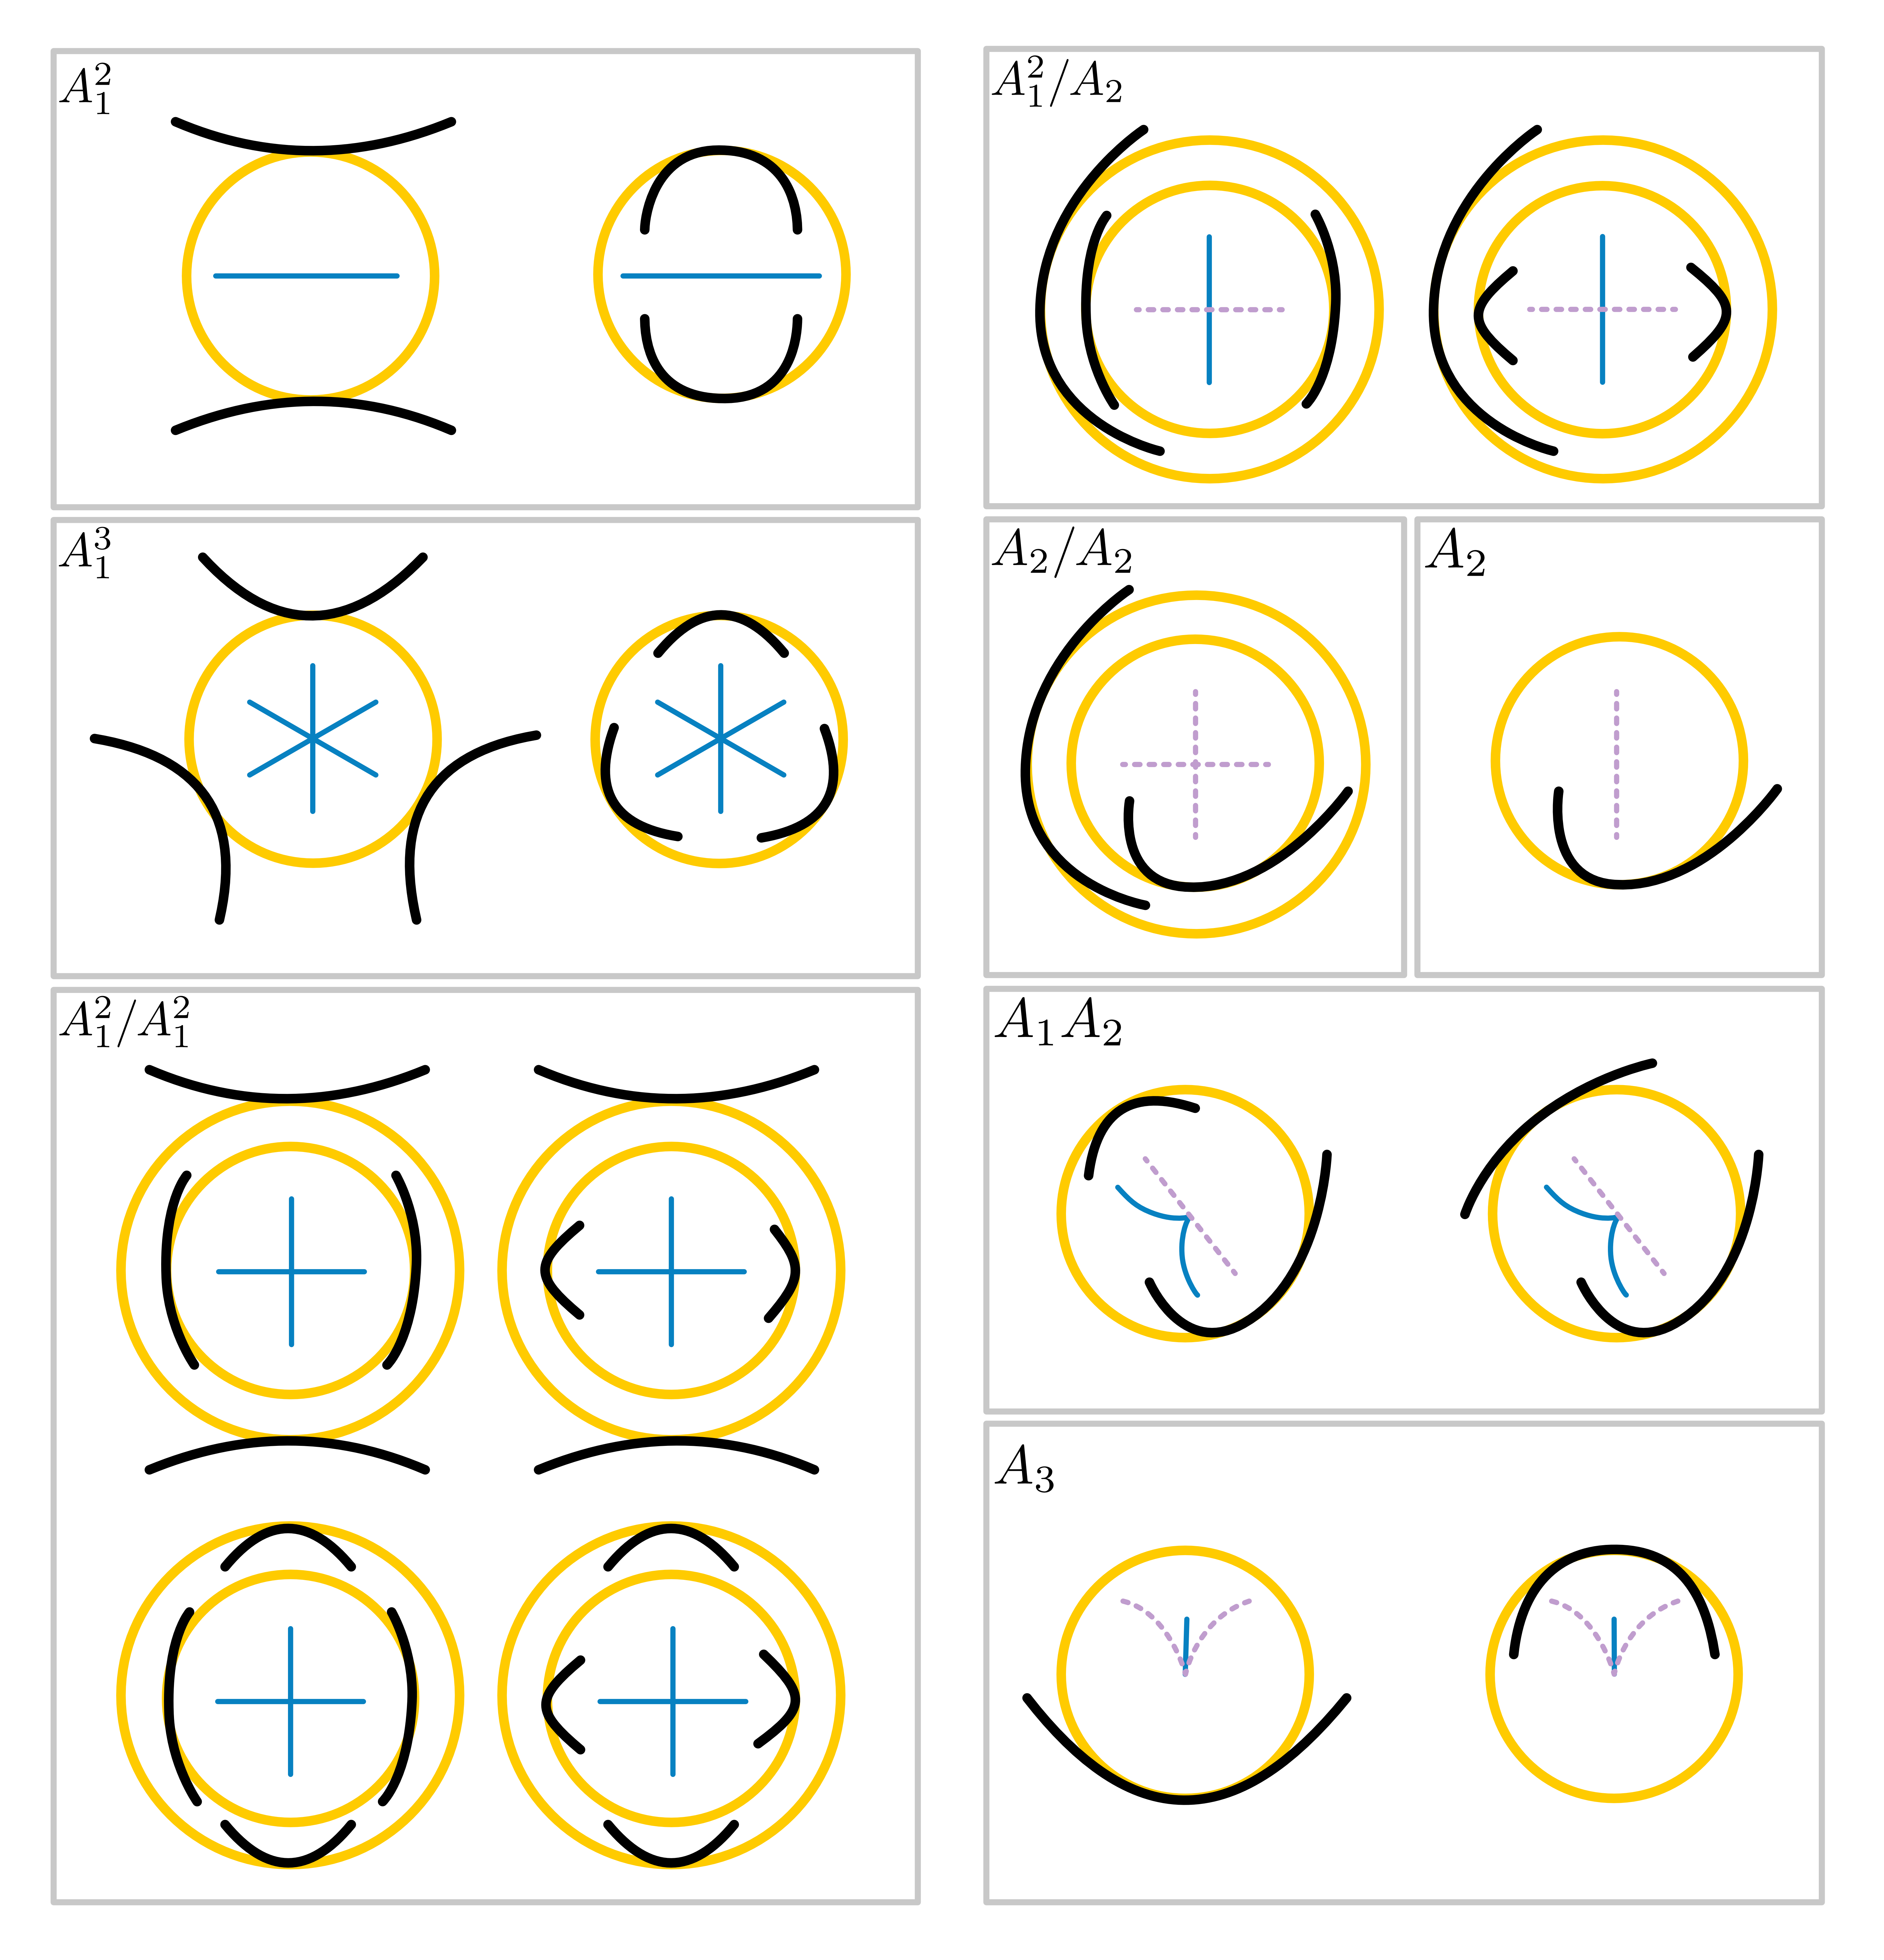
\includegraphics[width=0.45\linewidth]{Singularities_labeled_cropped.png}
    \end{figure}
\end{frame}


\begin{frame}{Classification $\Rightarrow$ a single culprit}
    \begin{columns}[T]
        \begin{column}{0.58\textwidth}
            {\footnotesize
            \renewcommand{\arraystretch}{1.2}
            \begin{tabular}{@{}lc@{}}
                \toprule
                Type & Monodromy \\
                \midrule
                $A_1^2$ (bitangent circle) & no \\
                $A_1^3$ (triple tangency) & no \\
                $A_1^2/A_1^2$ (two concentric bitangents) & \textbf{yes} \\
                $A_2$ (osculating; focal) & no \\
                $A_1A_2$ & no \\
                $A_3$ (curvature extremum) & no \\
                $A_1^2/A_2$ & no \\
                $A_2/A_2$ & no \\
                \bottomrule
            \end{tabular}}
        \end{column}
        \begin{column}{0.42\textwidth}
            \begin{block}{Main theorem (P2, P3)}
                {\footnotesize A generic small loop $\gamma$ has \textbf{no}
                nontrivial monodromy \emph{unless} its interior contains an
                $A_1^2/A_1^2$ singularity of the symmetry set. Otherwise the
                vineyard is $k$ unlinked circles.}
            \end{block}
        \end{column}
    \end{columns}
    \vspace{0.7em}
    \pause
    While with large loops it is a bit more complicated, an $A_2/A_2$ singularity can be the cause of monodromy.
    % {\footnotesize Every ``no'' either reorders without re-pairing, or only creates
    % a low-persistence near-diagonal pair. }
    % First work to combine symmetry sets +
    % persistence + singularity theory.}
    % \note{State the theorem plainly. $A_1^2/A_1^2$ = transversal crossing of a
    % birth-birth and a death-death piece. ~2 min.}
\end{frame}

\begin{frame}{Two facts that make the theory work}
    \begin{enumerate}
        \item \textbf{Stability outside $\gsym(\M)$.} On a component of $\R^2\setminus\gsym(\M)$ the combinatorics of the persistence diagram is stable. So a loop avoiding $\gsym(\M)$ gives $k$ \textbf{unlinked circles} --- no monodromy. All monodromy comes from singularities.
        \item \textbf{The interchange mechanism.} Two vines can swap only if $\gamma$ crosses both a \emph{birth--birth} and a \emph{death--death} stratum ($\ge 4$ contact points, exactly two pairs).
    \end{enumerate}
    \vspace{0.3em}
    {\footnotesize Reordering of critical values always happens; the \textbf{elder
    rule} can additionally change the pairing (producing ``knees''). Both together
    are needed for monodromy.}
    \note{The backbone. Only geometry crossing birth-birth AND death-death can
    braid. ~2 min.}
\end{frame}

% \begin{frame}{Local $\ne$ global: a cautionary example}
%     \begin{columns}[T]
%         \begin{column}{0.5\textwidth}
%             \centering
%             \includegraphics[width=0.82\linewidth]{A12A12_bigloop.pdf}\\
%             {\scriptsize A large loop around a monodromy-generating $A_1^2/A_1^2$
%             --- \emph{no} monodromy.}
%         \end{column}
%         \begin{column}{0.5\textwidth}
%             \centering
%             \includegraphics[width=0.72\linewidth]{bishop_staff2.pdf}\\
%             {\scriptsize A large loop with an $A_2/A_2$ --- monodromy.}
%         \end{column}
%     \end{columns}
%     \vspace{0.2em}
%     {\footnotesize Singularities do \textbf{not} simply compose. Manuscript in
%     progress: a large loop with neither $A_1^2/A_1^2$ nor $A_2/A_2$ inside has no
%     monodromy and unlinked vines.}
%     \note{Message: the local theorem does not naively globalise -- the next paper.
%     ~1.5 min.}
% \end{frame}

%========================================================================
\section{Bouquet2D: the tool}
%========================================================================

\begin{frame}{Why build a tool? -- Bouquet2D}
    \begin{columns}[T]
        \begin{column}{0.6\textwidth}
            % The tool was made for:
            % \begin{itemize}
            %     \item \textbf{Validation:} check the theorems on explicit examples.
            %     \item \textbf{Exploration:} deform a shape and watch the vineyard
            %           react --- generate conjectures.
            %     \item \textbf{Communication:} generate pretty pictures!
            % \end{itemize}
            \vspace{4em}
            \textbf{Bouquet2D} was made for exporing this connection between the bifurcation set and the topology of the vineyard interactively and visually.\\
            % {\footnotesize\url{https://bouquet2d.rohitroy.me}}
        \end{column}
        \begin{column}{0.4\textwidth}
            \centering
            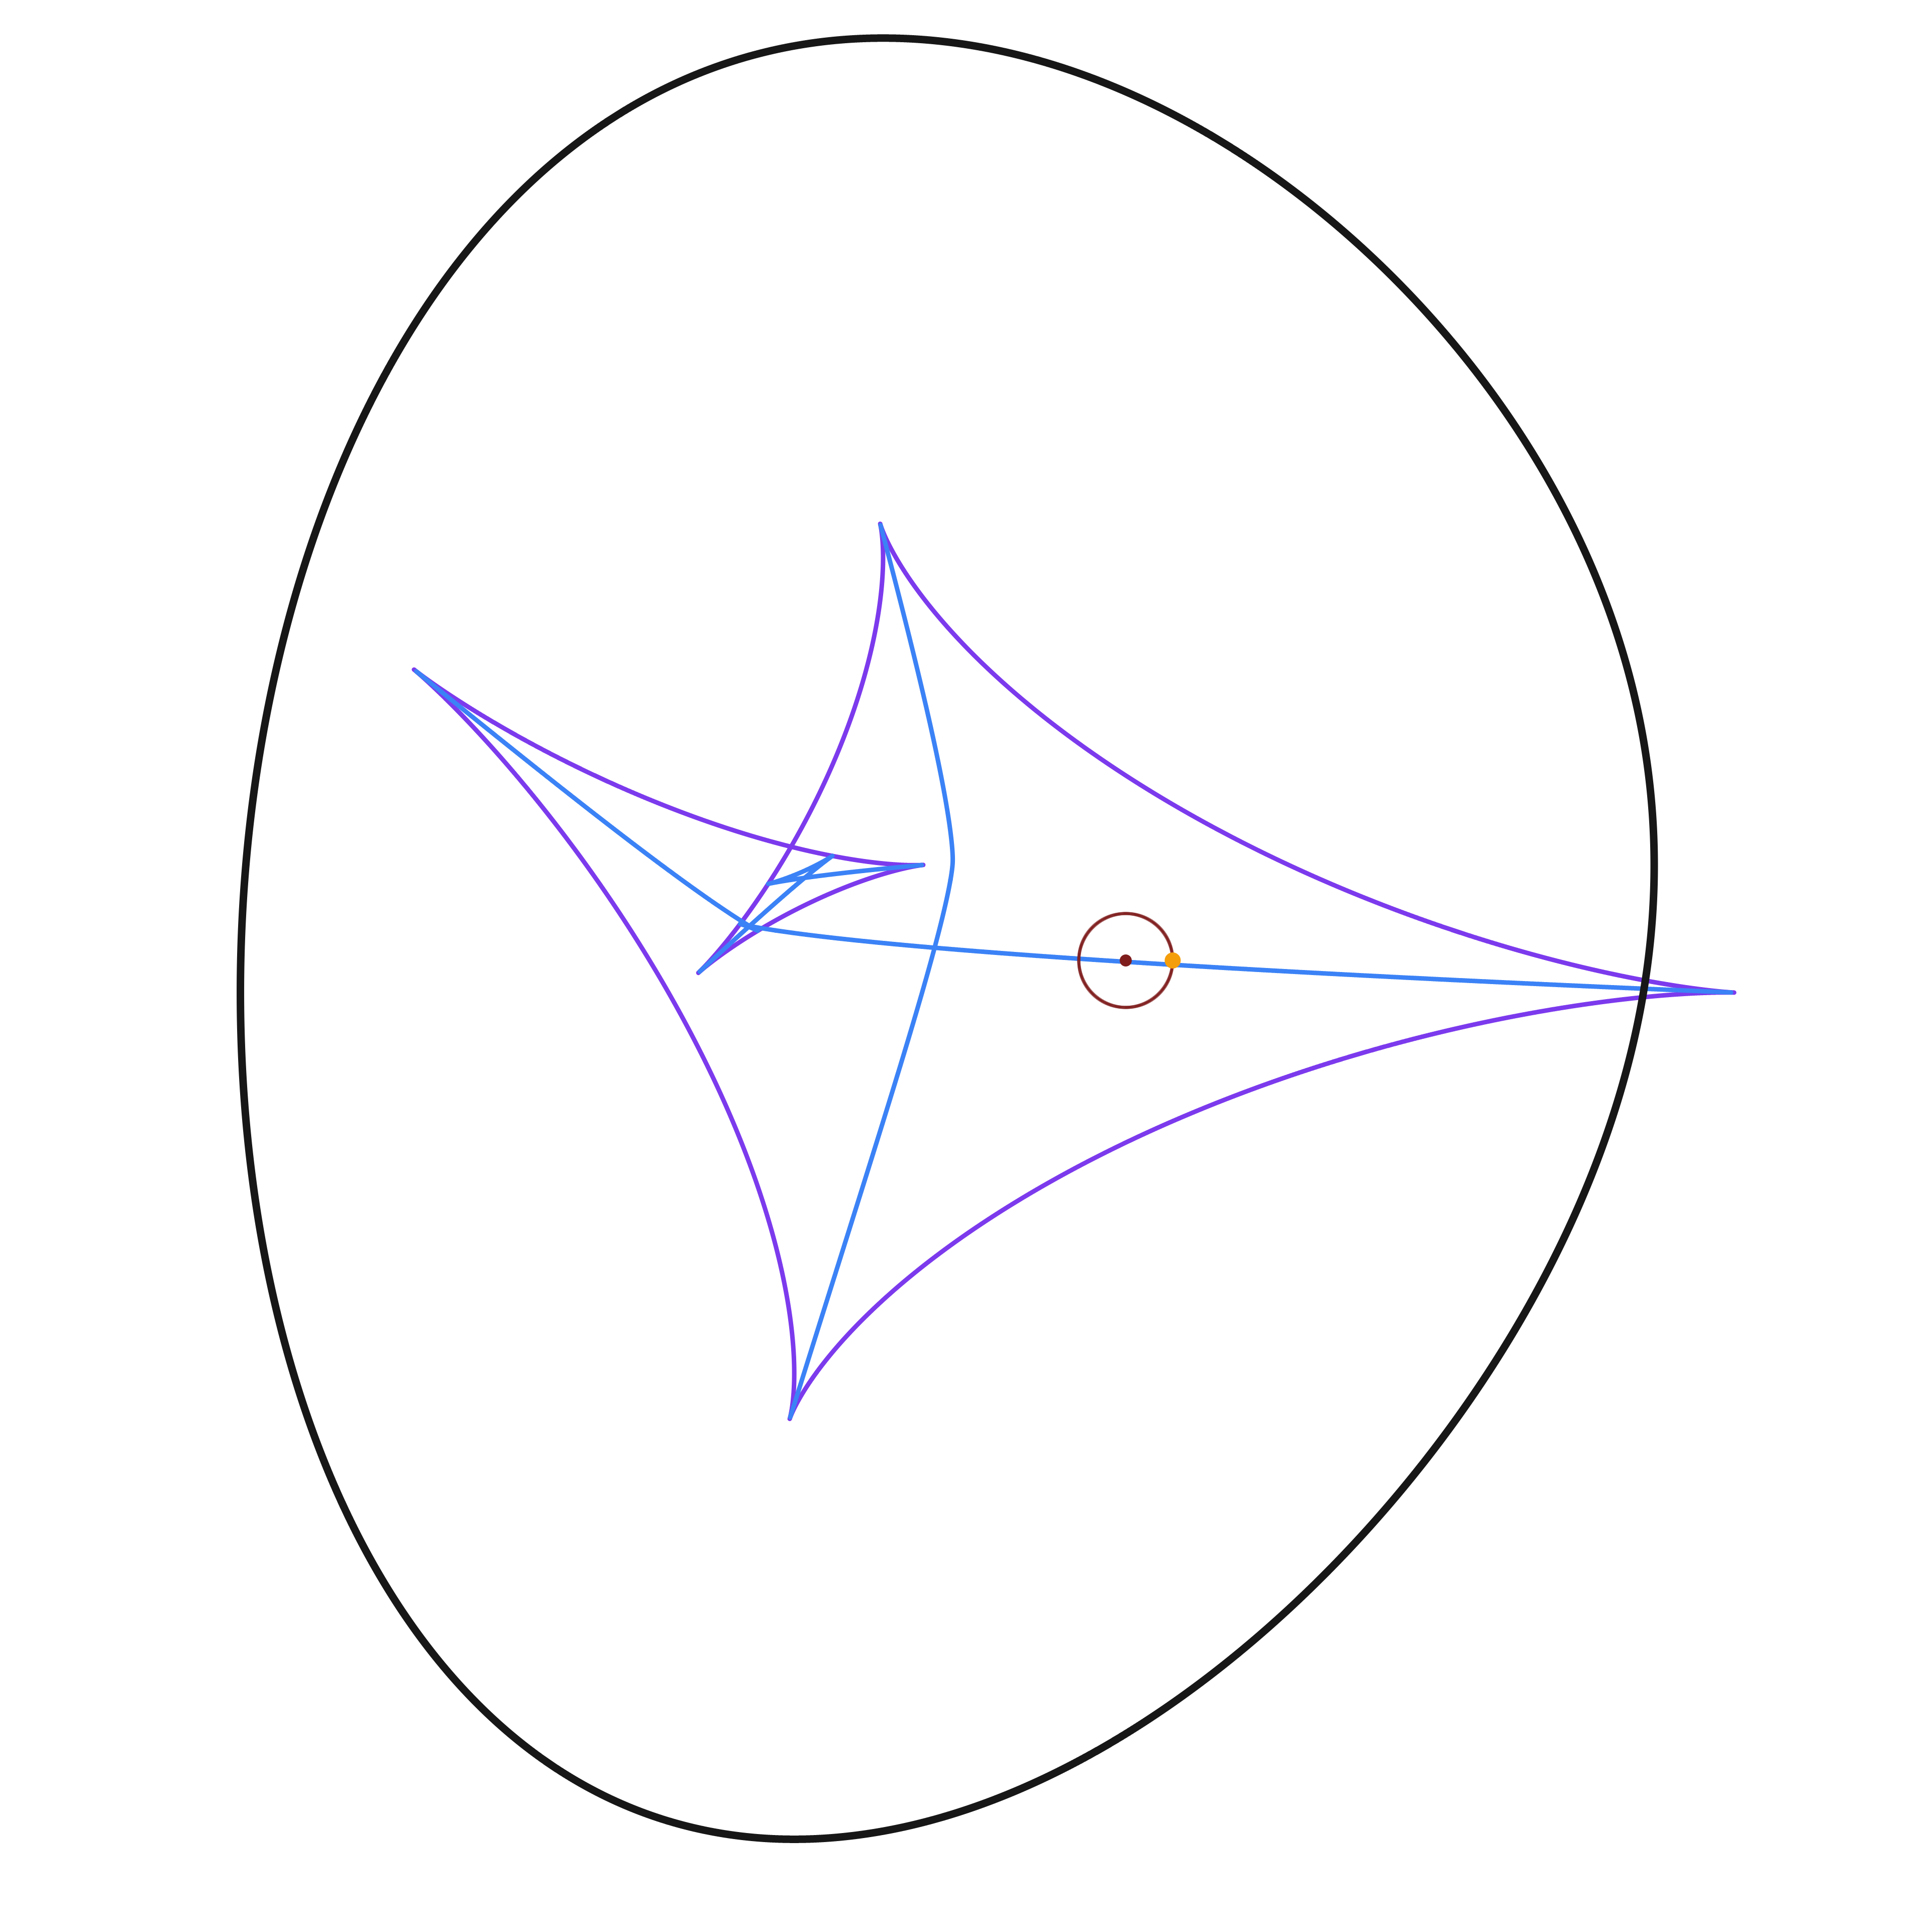
\includegraphics[width=\linewidth]{potato_eg.png}\\
            % {\scriptsize A spline curve with its symmetry \& focal sets.}
        \end{column}
    \end{columns}
    \note{Pivot to the tool -- the heart of the talk. ~1 min.}
\end{frame}

\begin{frame}{What Bouquet2D does}
    \textbf{Input:} a curve $\M$ as an editable spline; an observation loop
    (circle, or hand-drawn spline).\\[0.4em]
    \textbf{Computes and renders, in real time:}
    \begin{columns}[T]
        \begin{column}{0.30\textwidth}
            \centering
            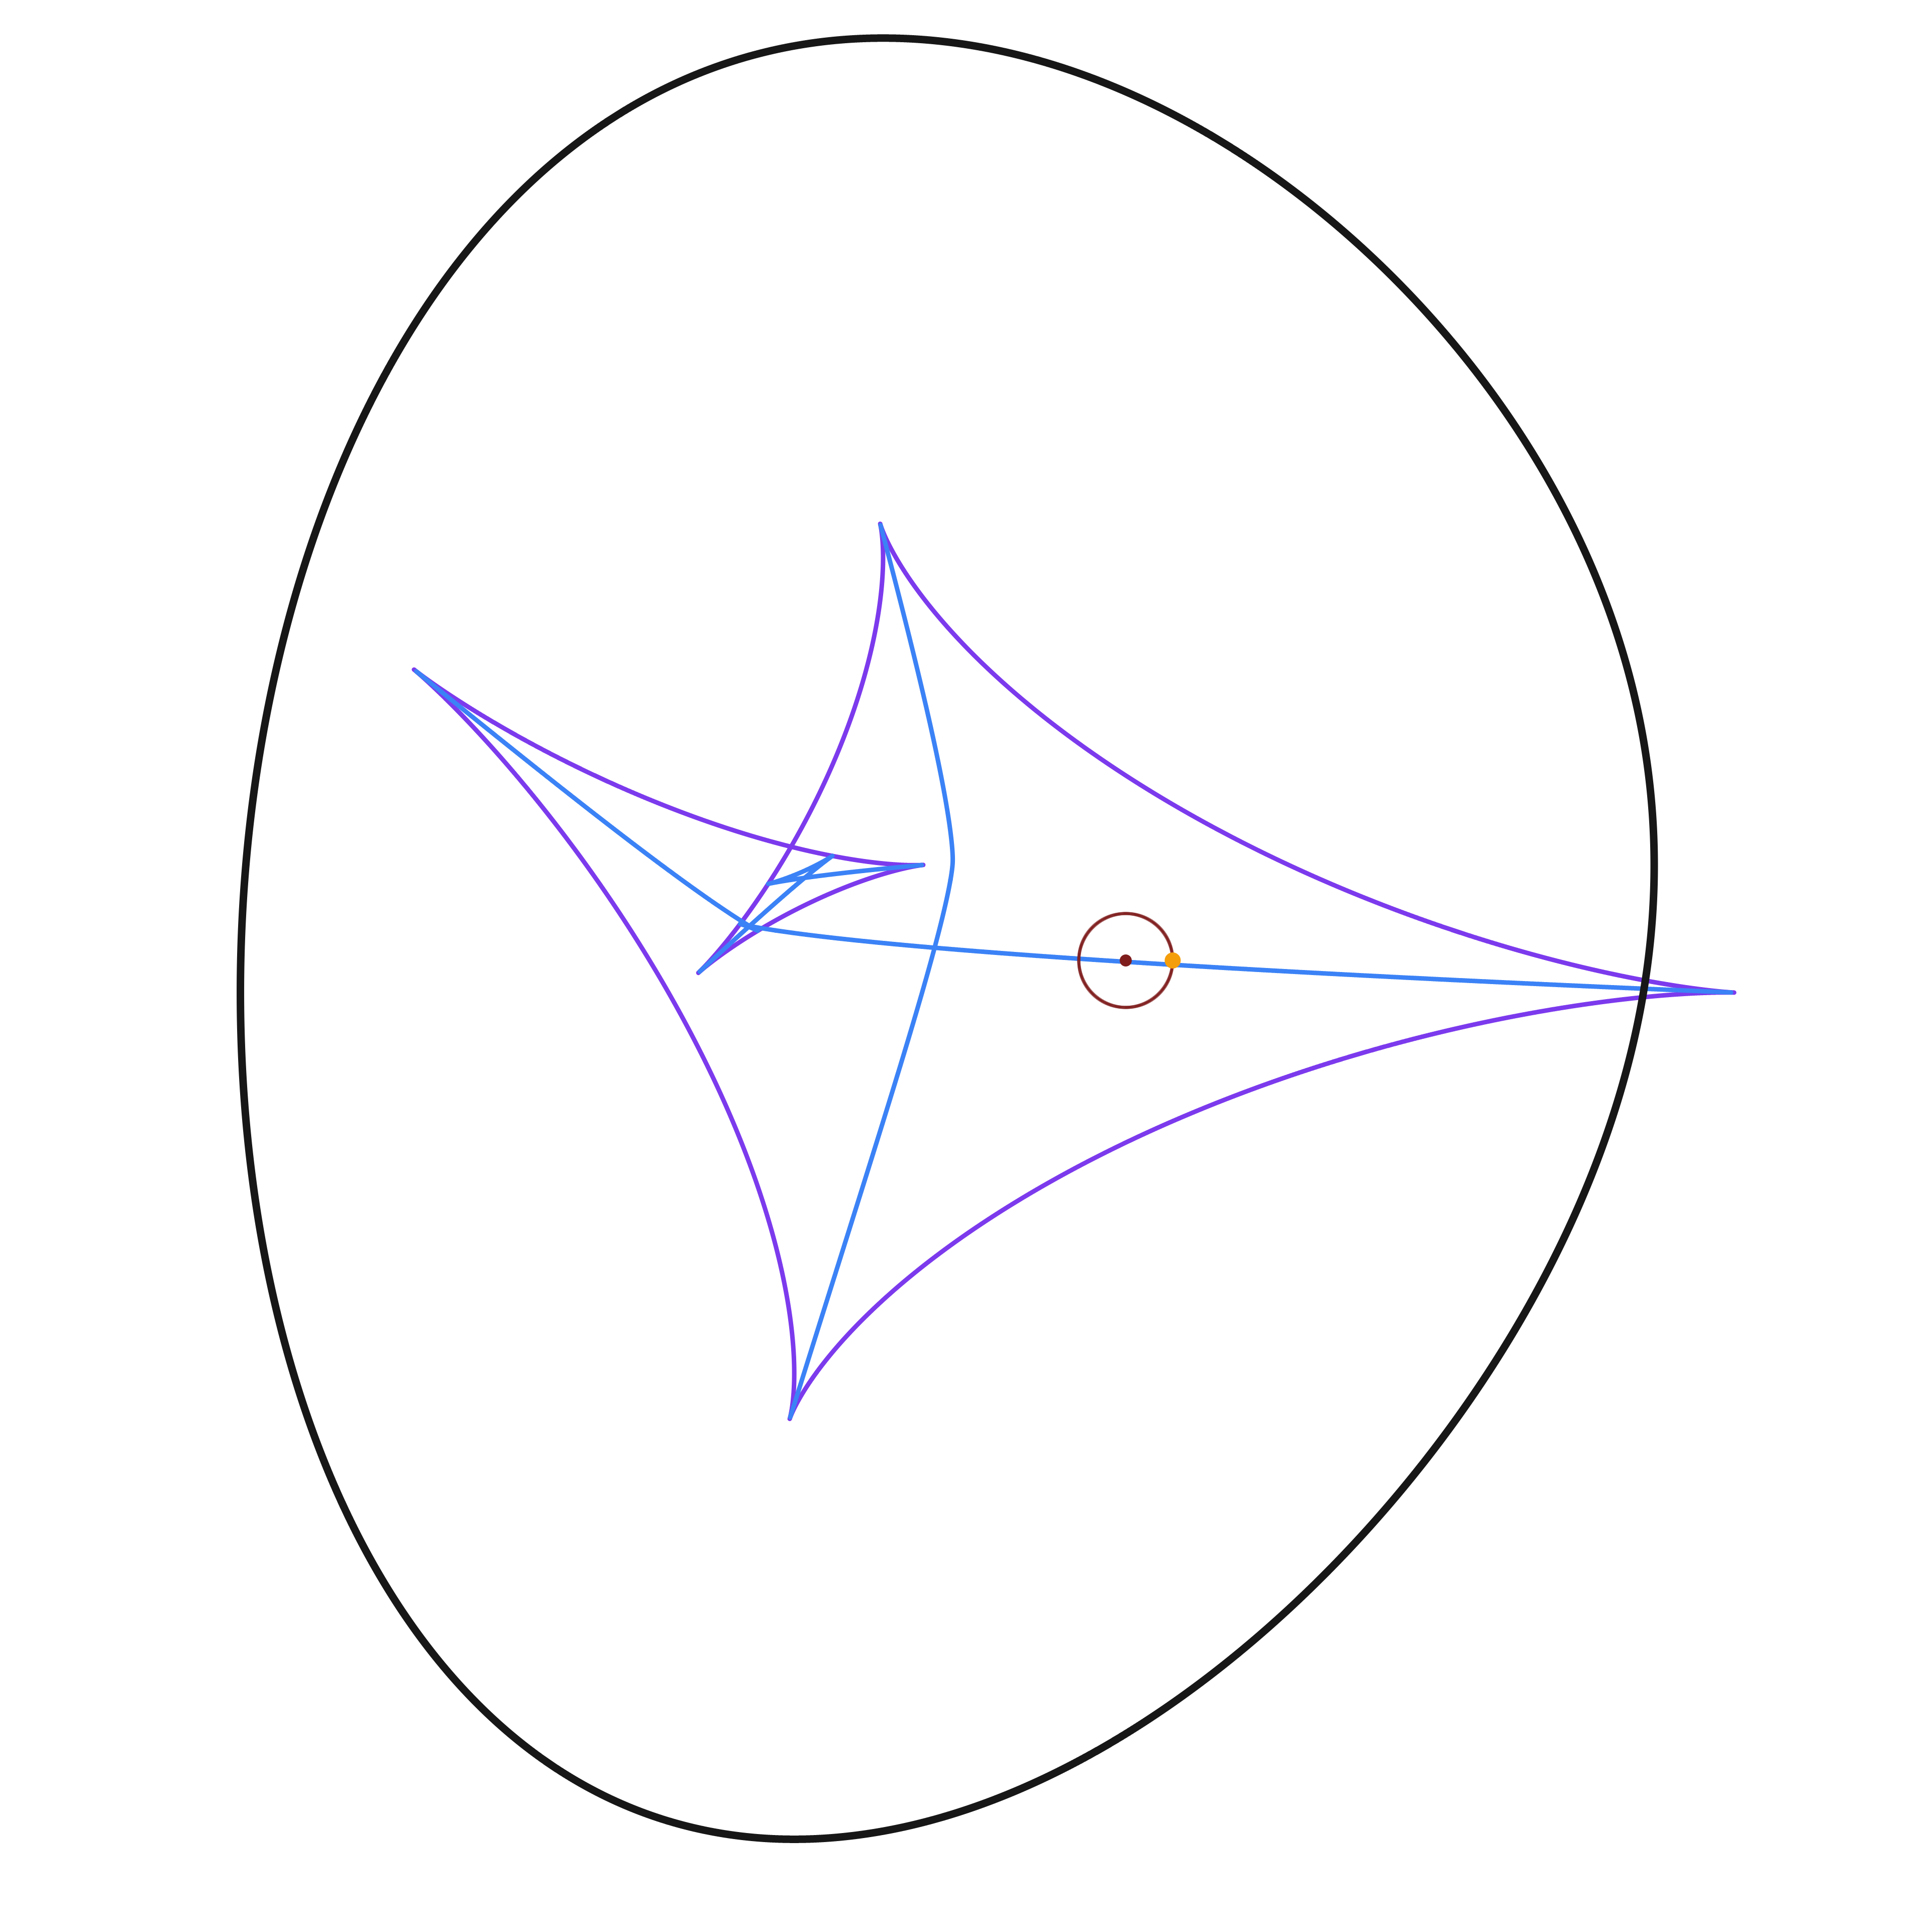
\includegraphics[width=\linewidth]{potato_eg.png}\\
            {\scriptsize focal + symmetry sets}
        \end{column}
        \begin{column}{0.33\textwidth}
            \centering
            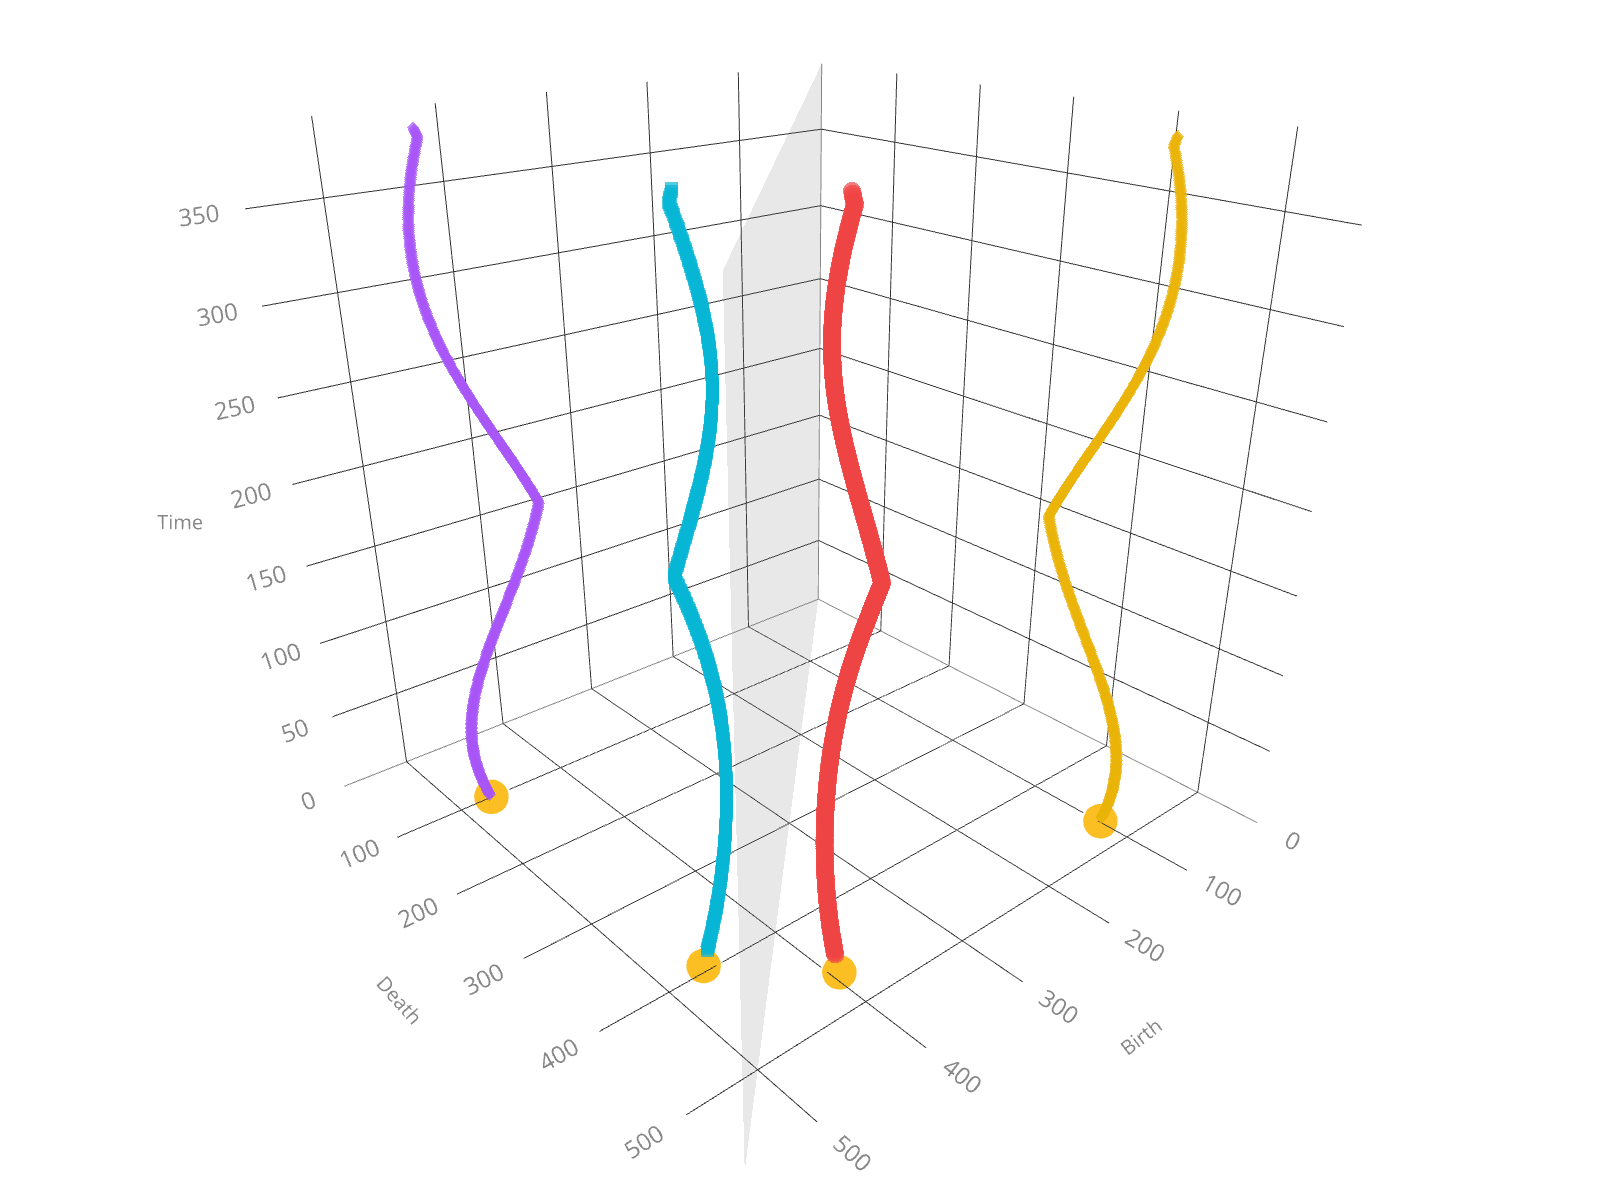
\includegraphics[width=\linewidth]{potato_vin.png}\\
            {\scriptsize the 3D vineyard}
        \end{column}
        \begin{column}{0.30\textwidth}
            \centering
            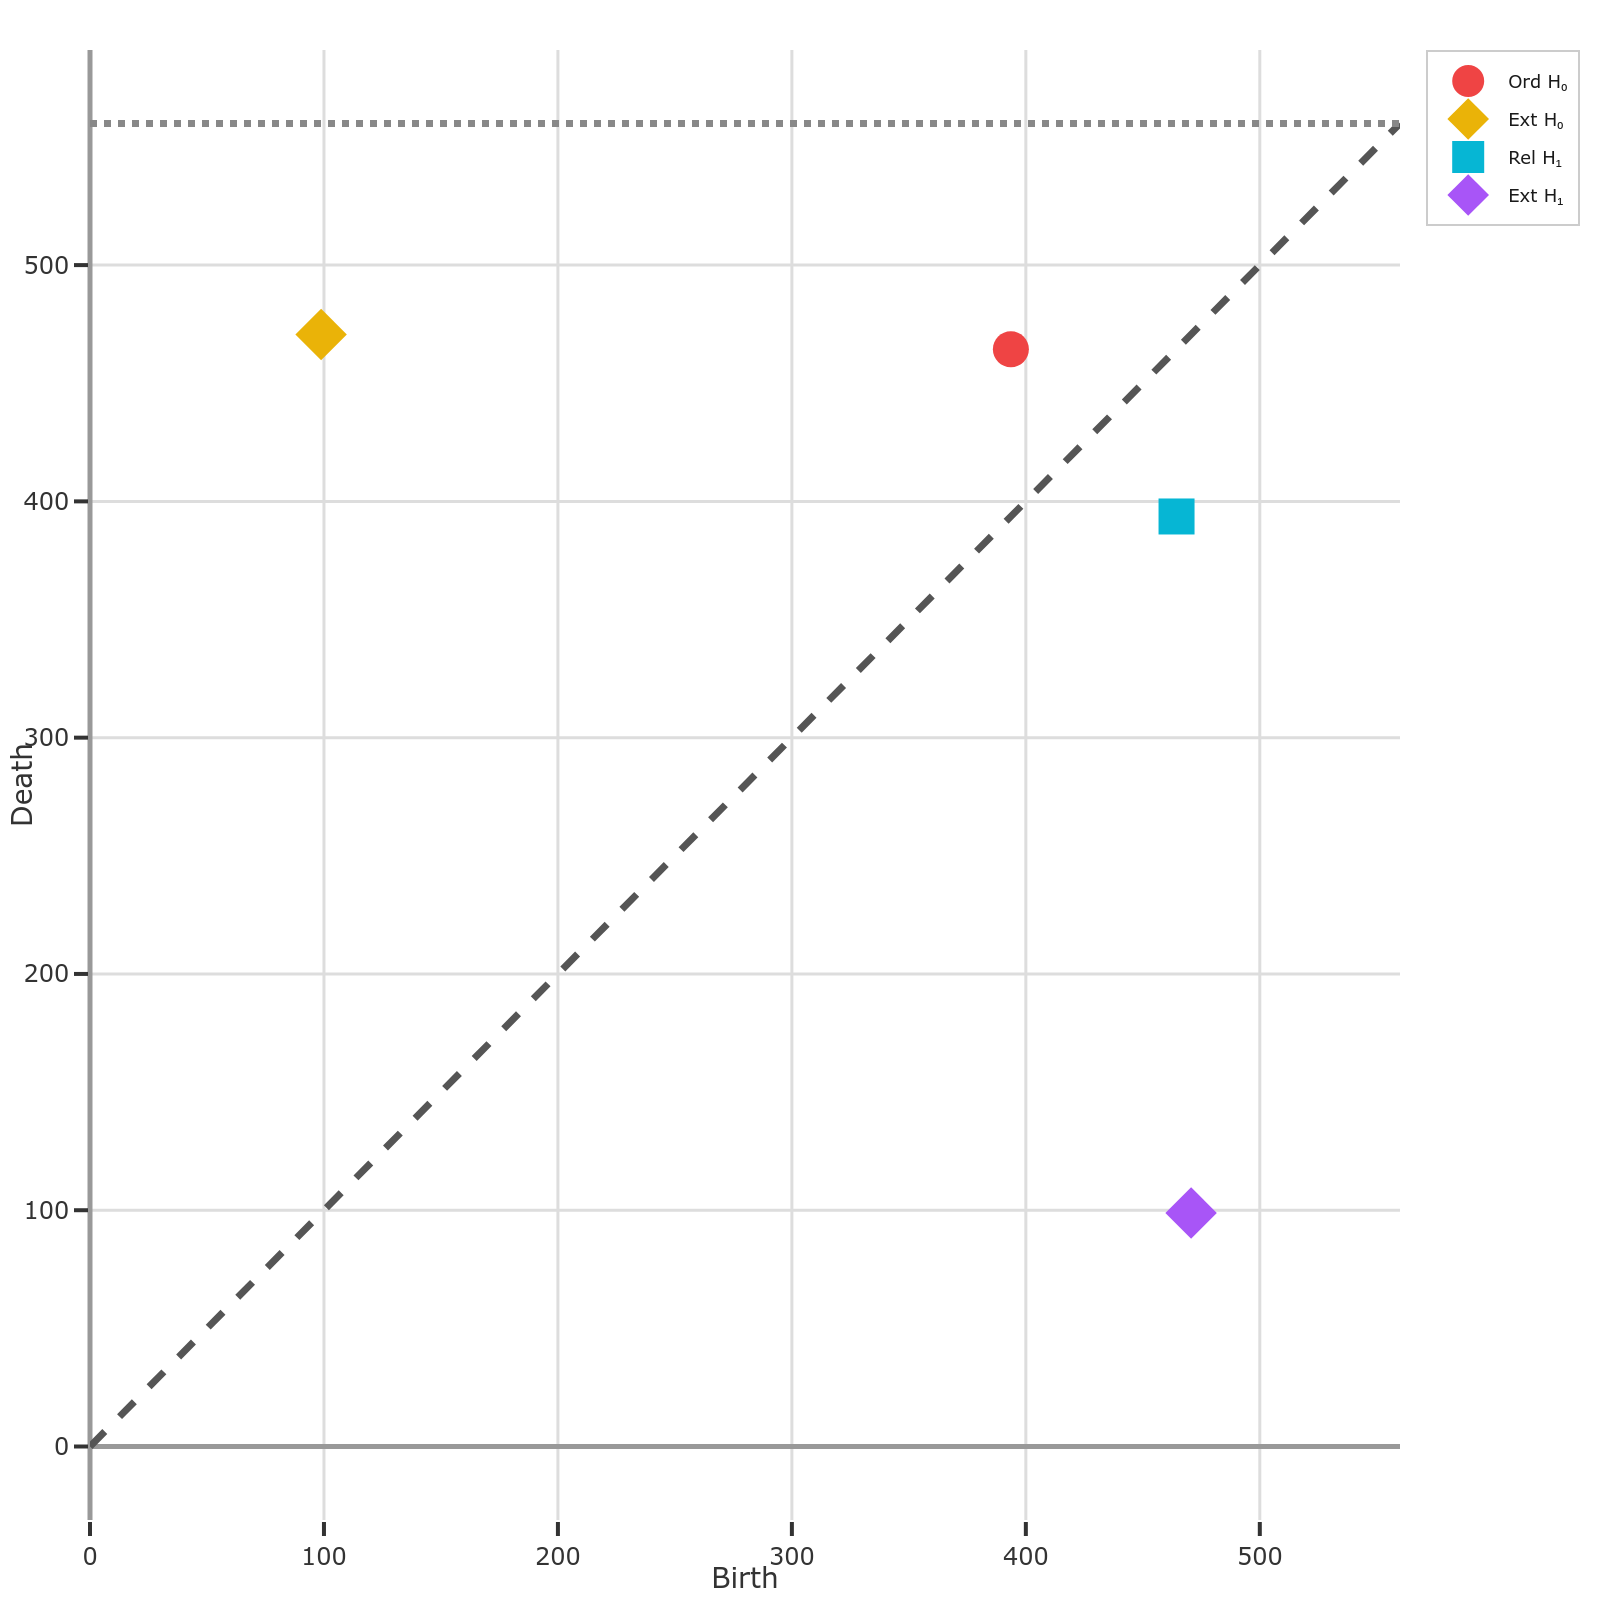
\includegraphics[width=\linewidth]{potato_pd.png}\\
            {\scriptsize the persistence diagram}
        \end{column}
    \end{columns}
    % \vspace{0.2em}
    % {\footnotesize Tip: swap these for a screenshot of the live UI if you have one.}
    % \note{One-slide I/O overview before the live demo. ~1 min.}
\end{frame}

% \begin{frame}{Under the hood I --- the symmetry set}
%     Following Bruce--Giblin--Gibson, from a sampled curve:
%     \begin{enumerate}
%         \item \textbf{Detect bitangencies} via sign changes of
%               $\;f_\pm(i,j) = (p_i - p_j)\cdot(t_i \pm t_j).$
%         \item \textbf{Locate the centre} by intersecting the normal lines at
%               $p_i,p_j$.
%         \item \textbf{Filter} by the equidistance test
%               $\bigl|\,\|C-p_i\|-\|C-p_j\|\,\bigr| < \epsilon_{\mathrm{rad}}$
%               to kill discretization artifacts.
%     \end{enumerate}
%     \vspace{0.3em}
%     {\footnotesize The focal set (evolute) comes directly from the curvature:
%     $E(s)=\gamma(s)+\rho(s)\,n(s)$.}
%     \note{The symmetry set is a discrete, sampling-based computation -- sets up the
%     limitations slide. ~1.5 min.}
% \end{frame}

% \begin{frame}{Under the hood II --- the vineyard}
%     For each sample $t$ of the observation loop:
%     \begin{itemize}
%         \item Build the lower-star filtration of $\dist^2(\cdot,\gamma(t))|_\M$.
%         \item A single \textbf{Union--Find} pass computes persistence via the
%               \textbf{elder rule}.
%         \item Collect $(t,\text{birth},\text{death})$ triples and \textbf{track}
%               them into vines.
%     \end{itemize}
%     \vspace{0.3em}
%     \begin{block}{Why so simple?}
%         In 1D the union-find pass is already fast enough for real-time interaction
%         --- no need for the general vineyard-update machinery.
%     \end{block}
%     \note{Contrast with heavy vineyard-update algorithms -- ours is deliberately
%     elementary because the setting is 1D. ~1.5 min.}
% \end{frame}

% \begin{frame}{Features worth showing}
%     \begin{columns}[T]
%         \begin{column}{0.5\textwidth}
%             \begin{itemize}
%                 \item Real-time \textbf{deformation} of the spline.
%                 \item \textbf{Circular} loops (adjustable centre/radius) or
%                       \textbf{hand-drawn} loops.
%                 \item \textbf{Extended persistence} (both sides of the diagonal).
%                 \item \textbf{Multiple components} + global bitangencies.
%                 \item Vineyard \textbf{breaks} exactly when the centre crosses the
%                       focal set.
%             \end{itemize}
%         \end{column}
%         \begin{column}{0.5\textwidth}
%             \centering
%             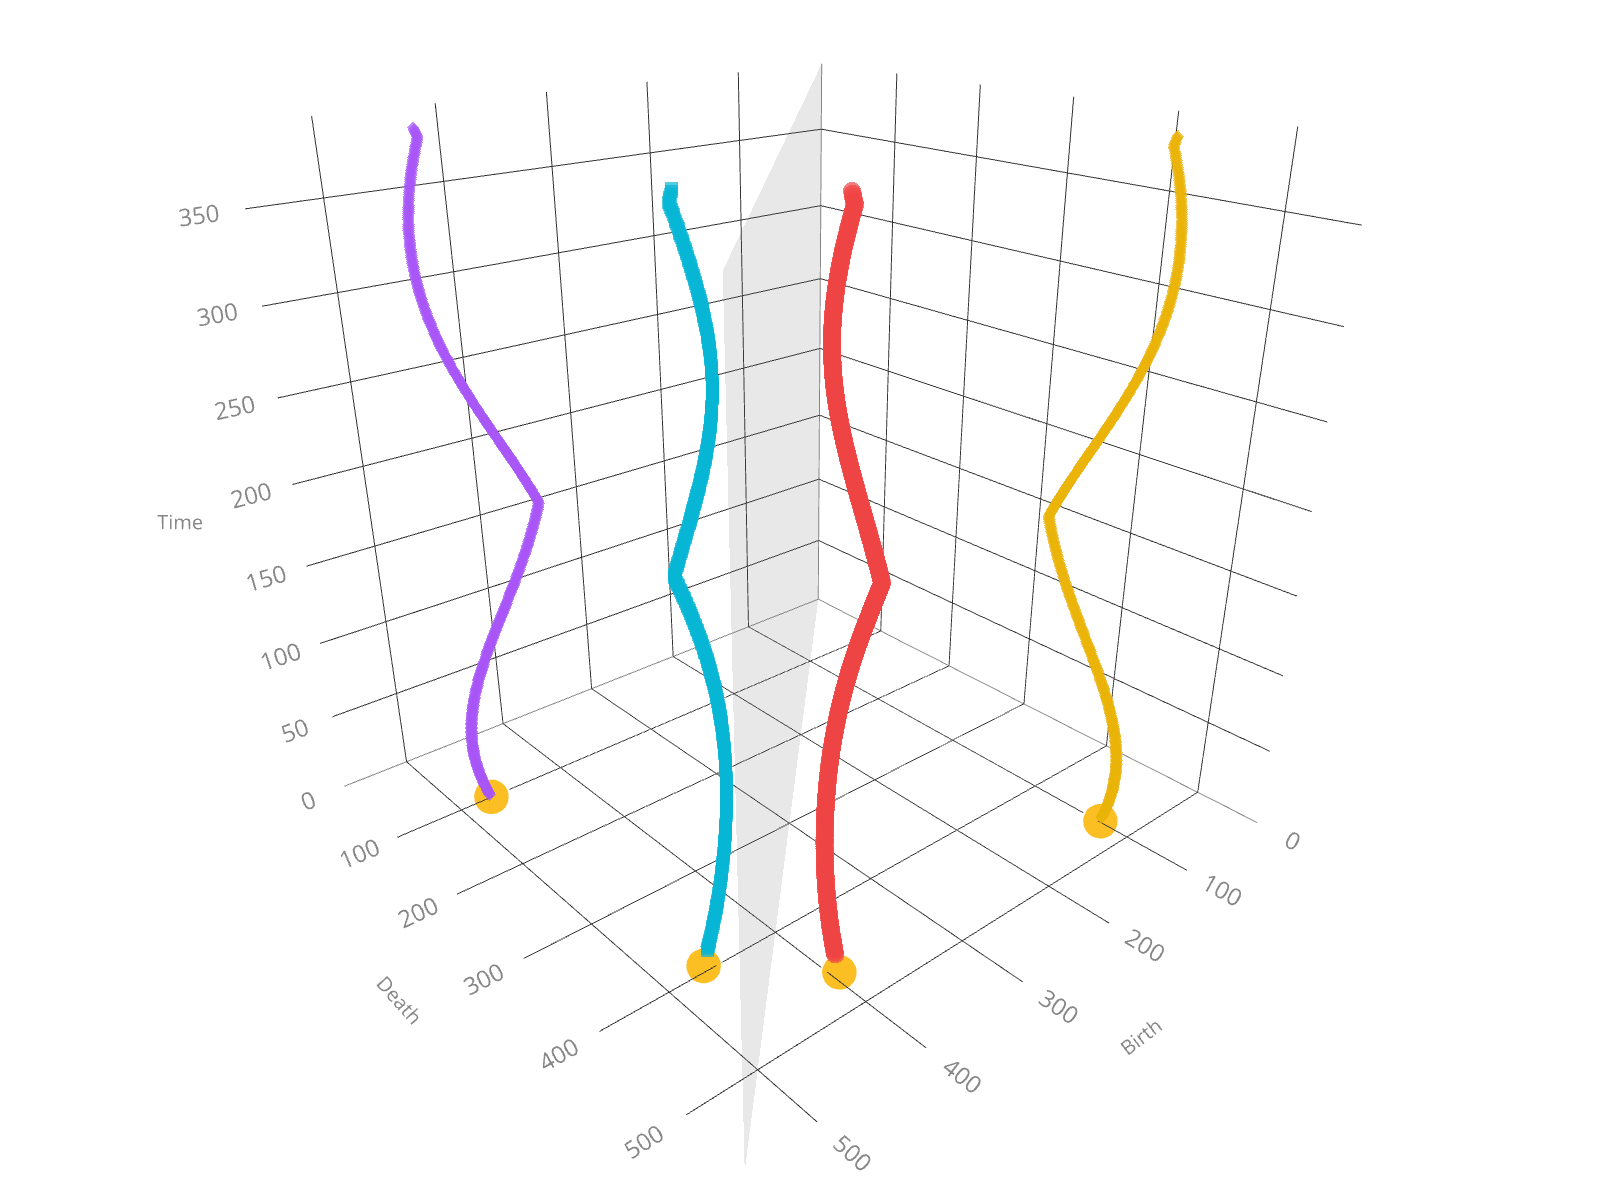
\includegraphics[width=\linewidth]{potato_vin.png}\\
%             {\scriptsize Vine breaking as the loop crosses the focal set.}
%         \end{column}
%     \end{columns}
%     \note{Things to click through live. Pick 3-4 to actually demonstrate. ~1 min.}
% \end{frame}

\begin{frame}{Bouquet2D -- Demo}
    % \vspace{0.3em}
    % \begin{block}{What I will show}
    %     \begin{itemize}
    %         \item Draw / deform a spline; watch symmetry \& focal sets update.
    %         \item Drop a circular loop; grow its radius across the focal set ---
    %               the vineyard \textbf{breaks} and reappears.
    %         \item Move the loop around an $A_1^2/A_1^2$ singularity --- the vines
    %               \textbf{interchange} (monodromy).
    %         \item Switch to a hand-drawn loop / two components.
    %     \end{itemize}
    % \end{block}
    \begin{center}
        {\url{https://bouquet2d.rohitroy.me}}
    \end{center}
    % \note{DEMO -- budget 5-8 minutes. Have the browser open with a saved example
    % (the deformed ellipse with the $A_1^2/A_1^2$). If the live tool fails, fall
    % back to the figures in the deck.}
\end{frame}

\begin{frame}{Limitations of Bouquet2D}
    \begin{itemize}
        \item \textbf{Planar only:} smooth curves in $\R^2$; no higher dimensions yet.
        \item \textbf{Sampling-sensitive:} the discrete symmetry set can miss or add branches near singularities if the curve is under-sampled.
        \item \textbf{Threshold-sensitive:} results near singularities depend on user-set constants.
        % \item \textbf{Not built for scale:} the elementary vineyard computation is
        %       1D by design.
    \end{itemize}
    % \note{Being upfront about limits is good for a committee. ~1 min.}
\end{frame}

%========================================================================
\section{Triangulation \& stratified meshing (StratMesh)}
%========================================================================

\begin{frame}{A second strand: triangulating submanifolds}
    Before we looked what the effect of singularities are on persistence. 
    \vspace{2em}

    In the future, we would want to use that to identify the singularities which we also want to triangulate, which brings us to the second part of the presentation.
\end{frame}

\begin{frame}{Triangulating submanifolds}
    Implementing the \textbf{Boissonnat--Kachanovich--Wintraecken} algorithm --- a quantified version of Whitney's method.

    % \textbf{Step 1:} Perturbing nearby vertices of the ambient triangulation away from the manifold
    \begin{center}
        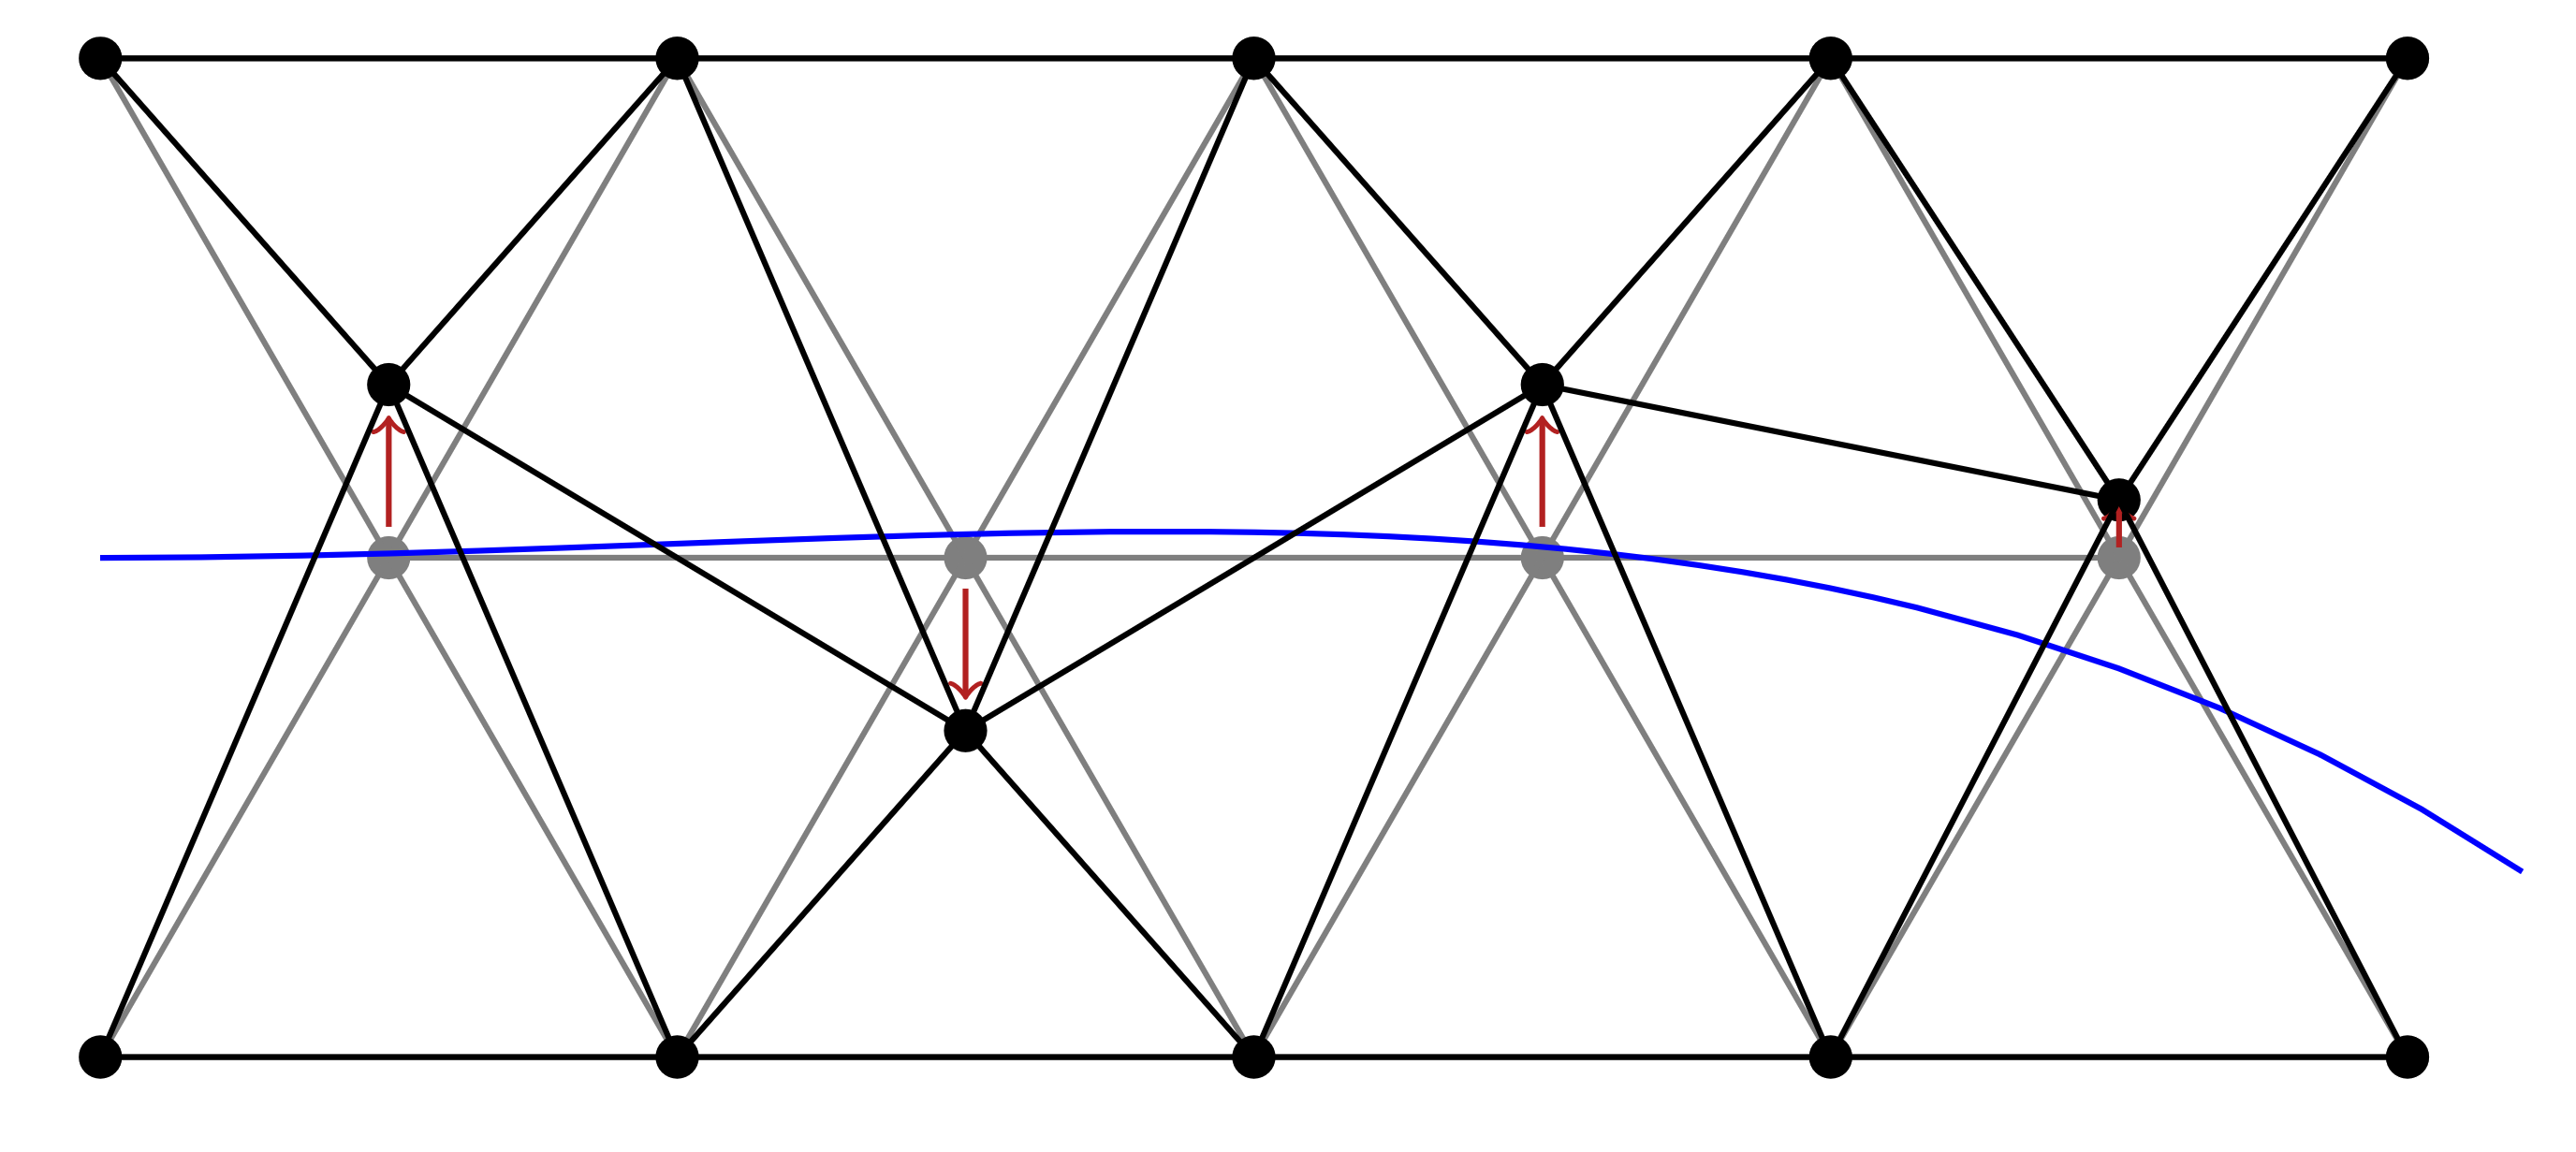
\includegraphics[width=0.66\linewidth]{triang1.png}
    \end{center}

    \vfill
    \bkwcite
\end{frame}

%------------------------------------------------------------------
% BKW algorithm, illustrated -- one figure per slide
%------------------------------------------------------------------
\begin{frame}{Triangulating submanifolds}
    \begin{center}
        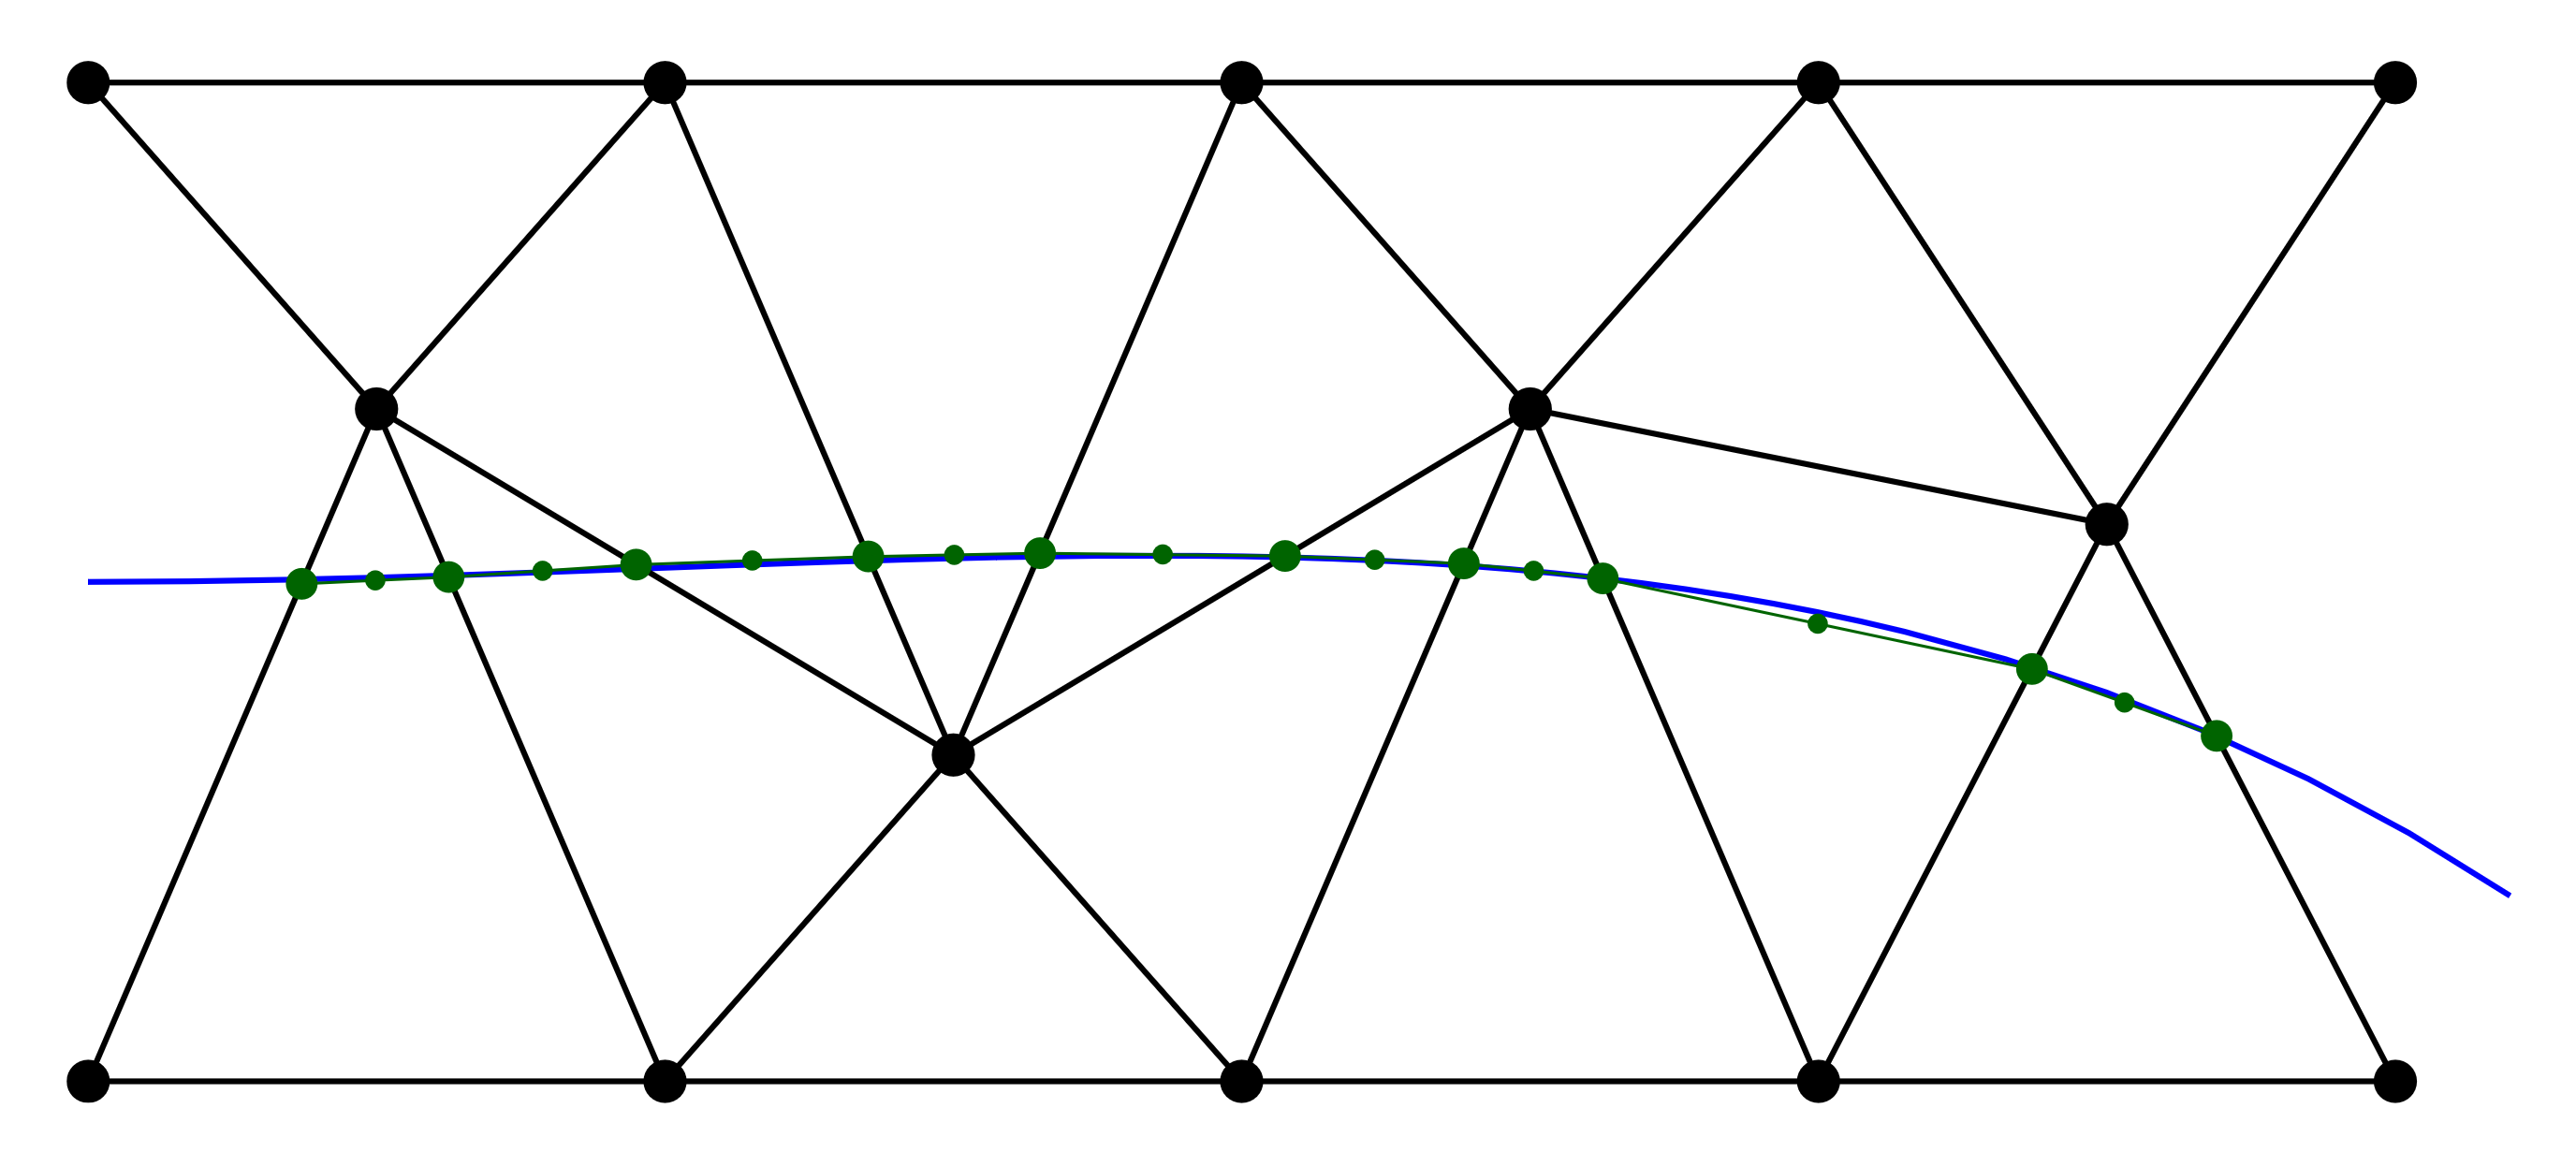
\includegraphics[width=0.8\linewidth]{triang2.png}
    \end{center}
    \vfill
    \bkwcite
\end{frame}

\begin{frame}{Triangulating submanifolds}
    \begin{center}
        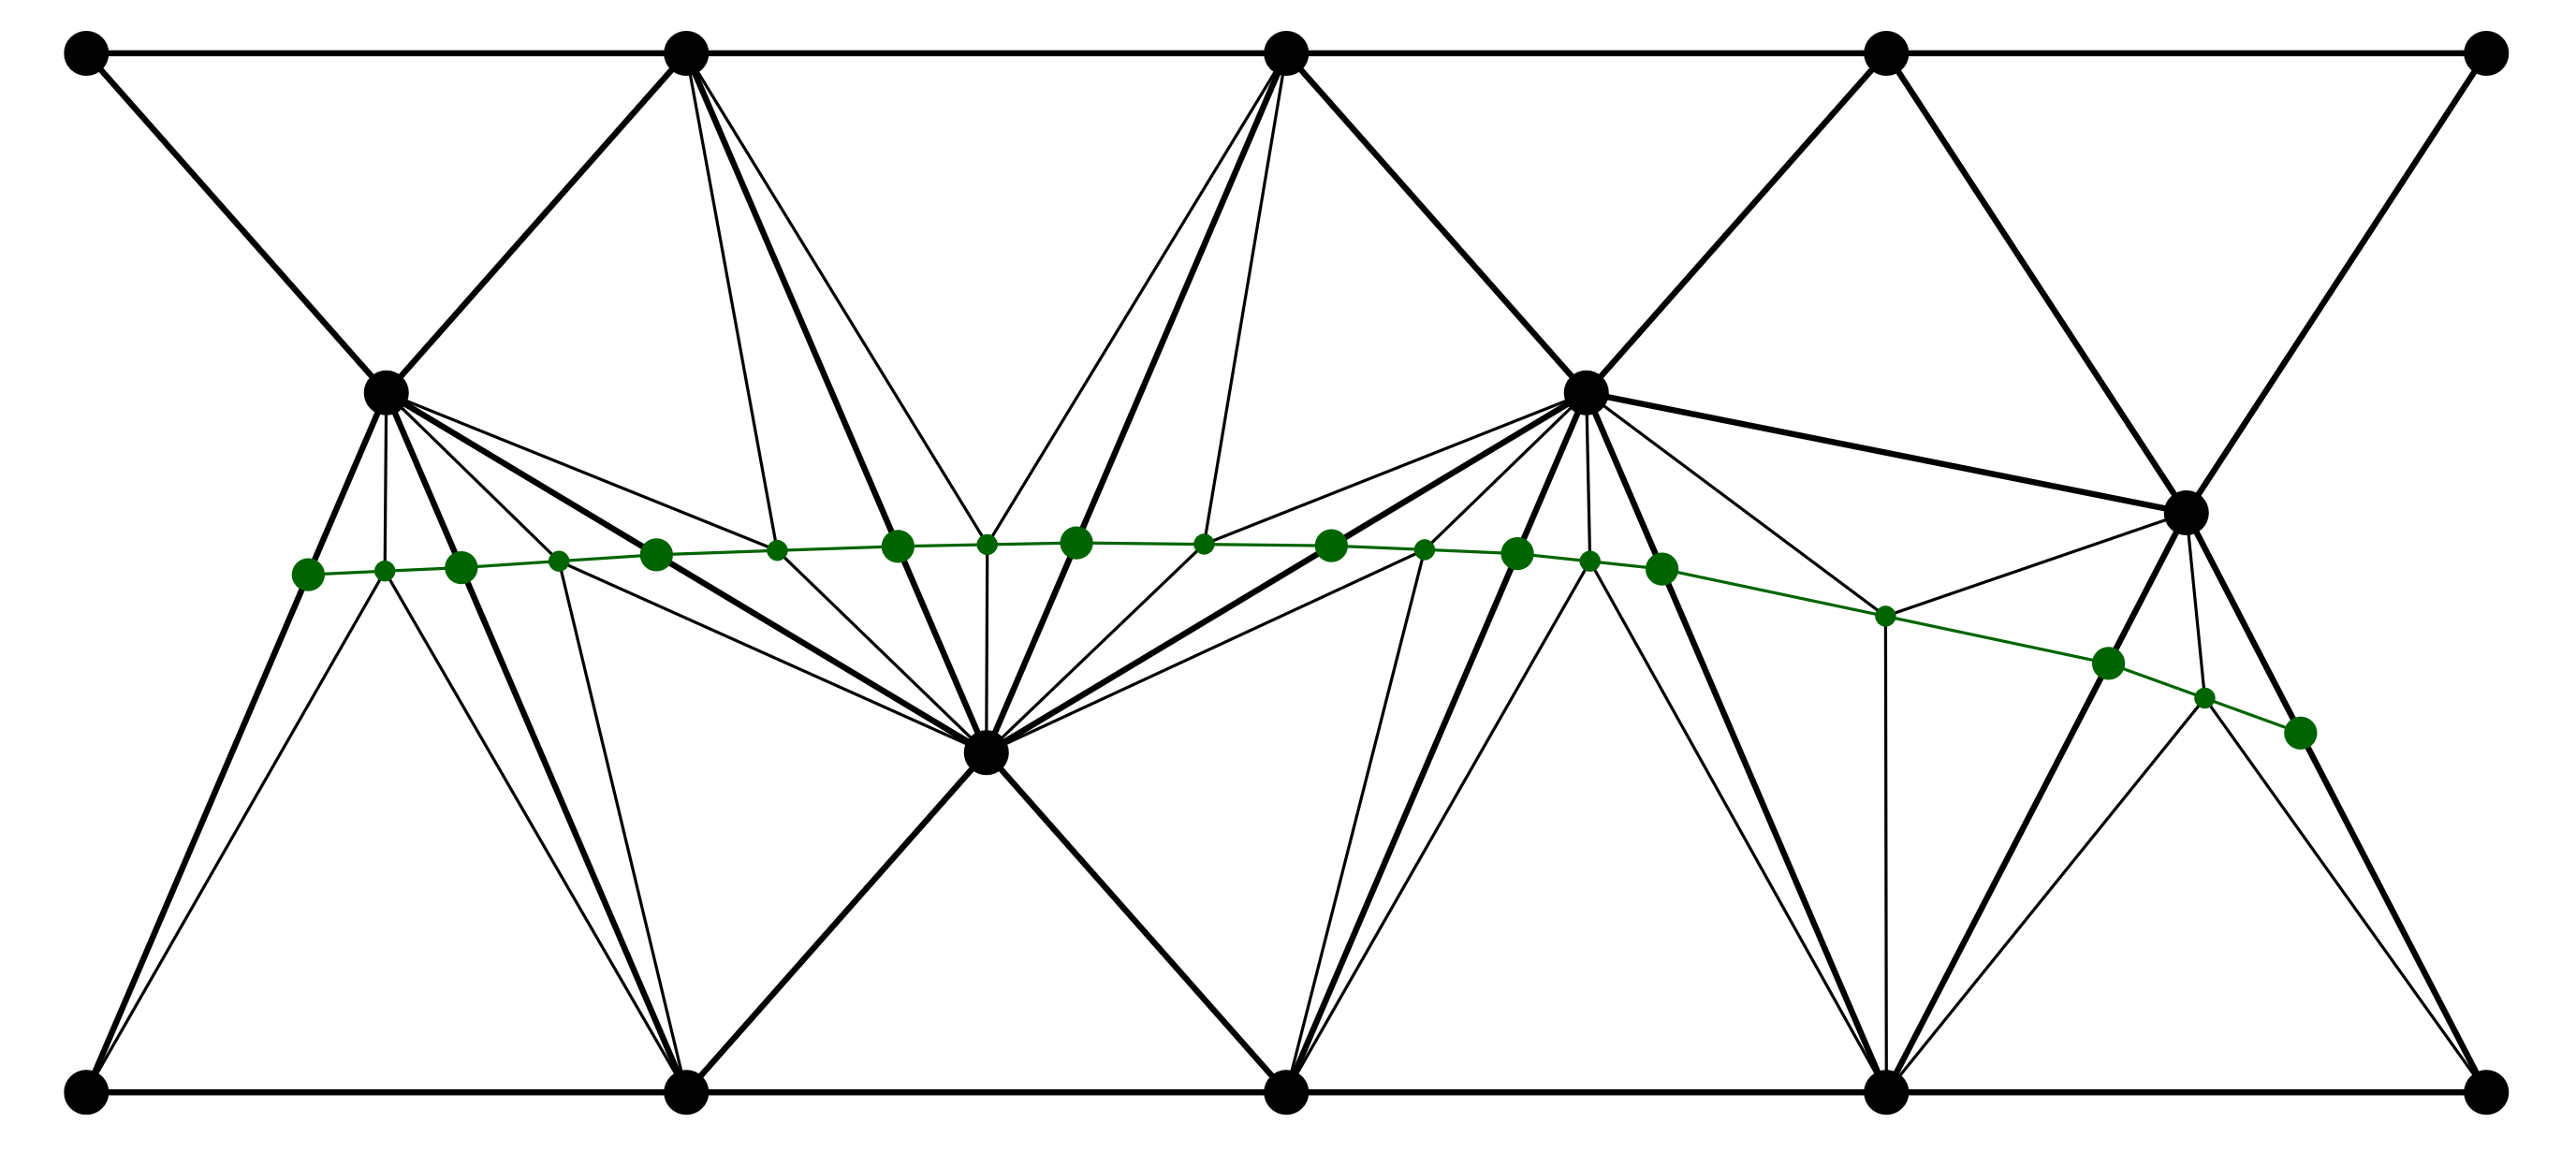
\includegraphics[width=0.8\linewidth]{triang3.png}
    \end{center}
    \vfill
    \bkwcite
\end{frame}

\begin{frame}{Triangulating submanifolds -- Obstacle!}
    \begin{itemize}
    
        \item Constants in the paper are extremely \textbf{small}, which are practically unusable.
        \item Trying out optimal constants that are practical for use.
    \end{itemize}

    \begin{figure}
    \centering
    \fbox{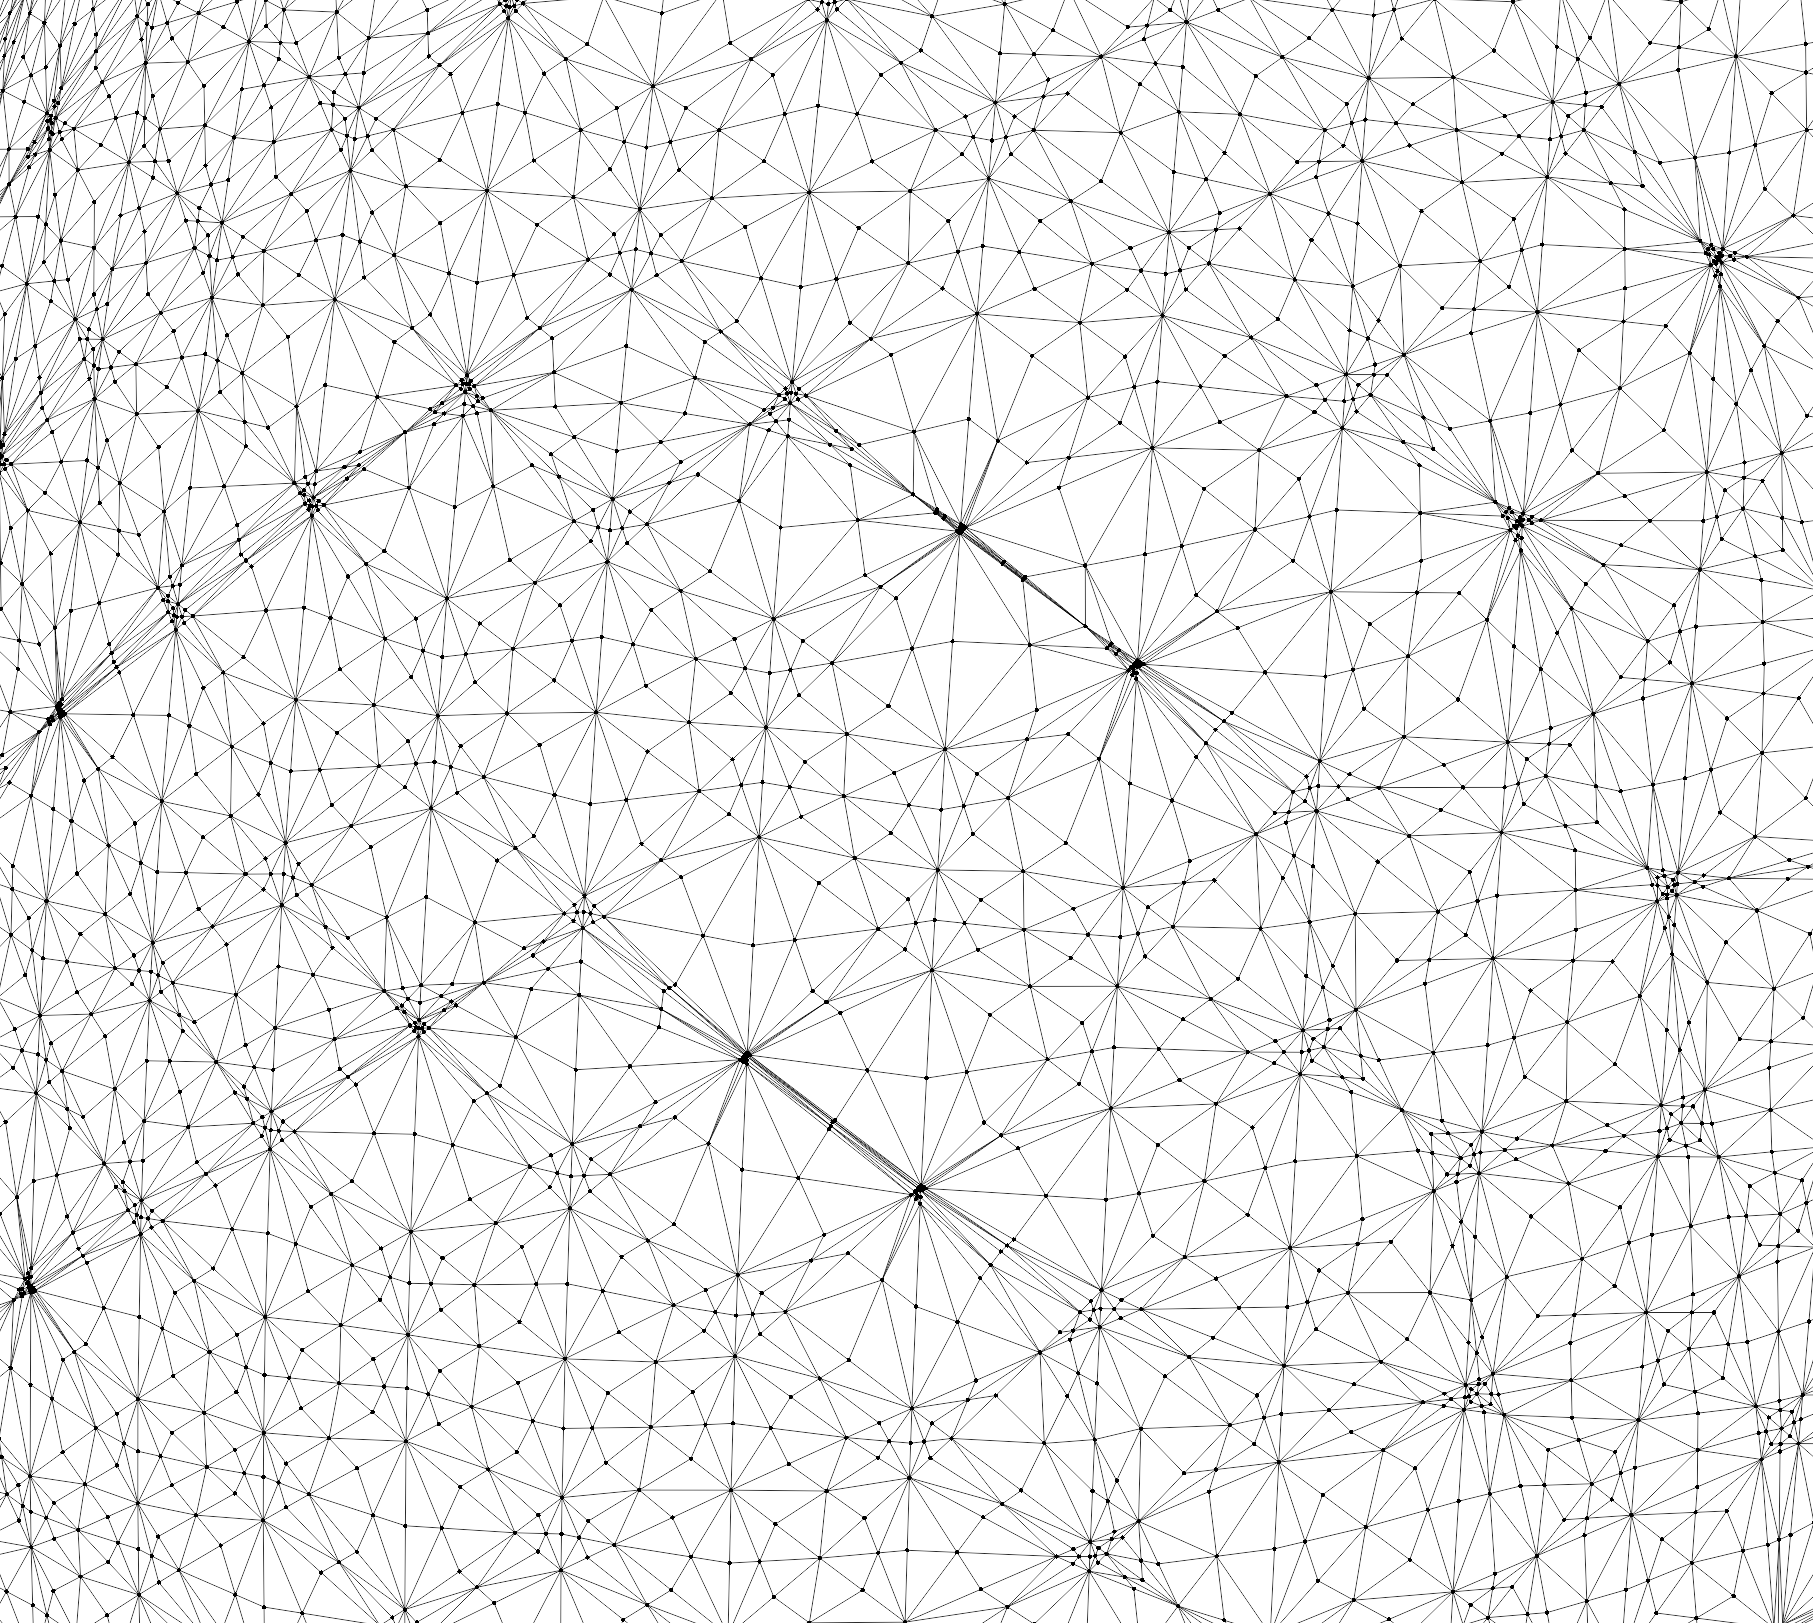
\includegraphics[width=0.35\linewidth]{torus_bad.png}}
    % 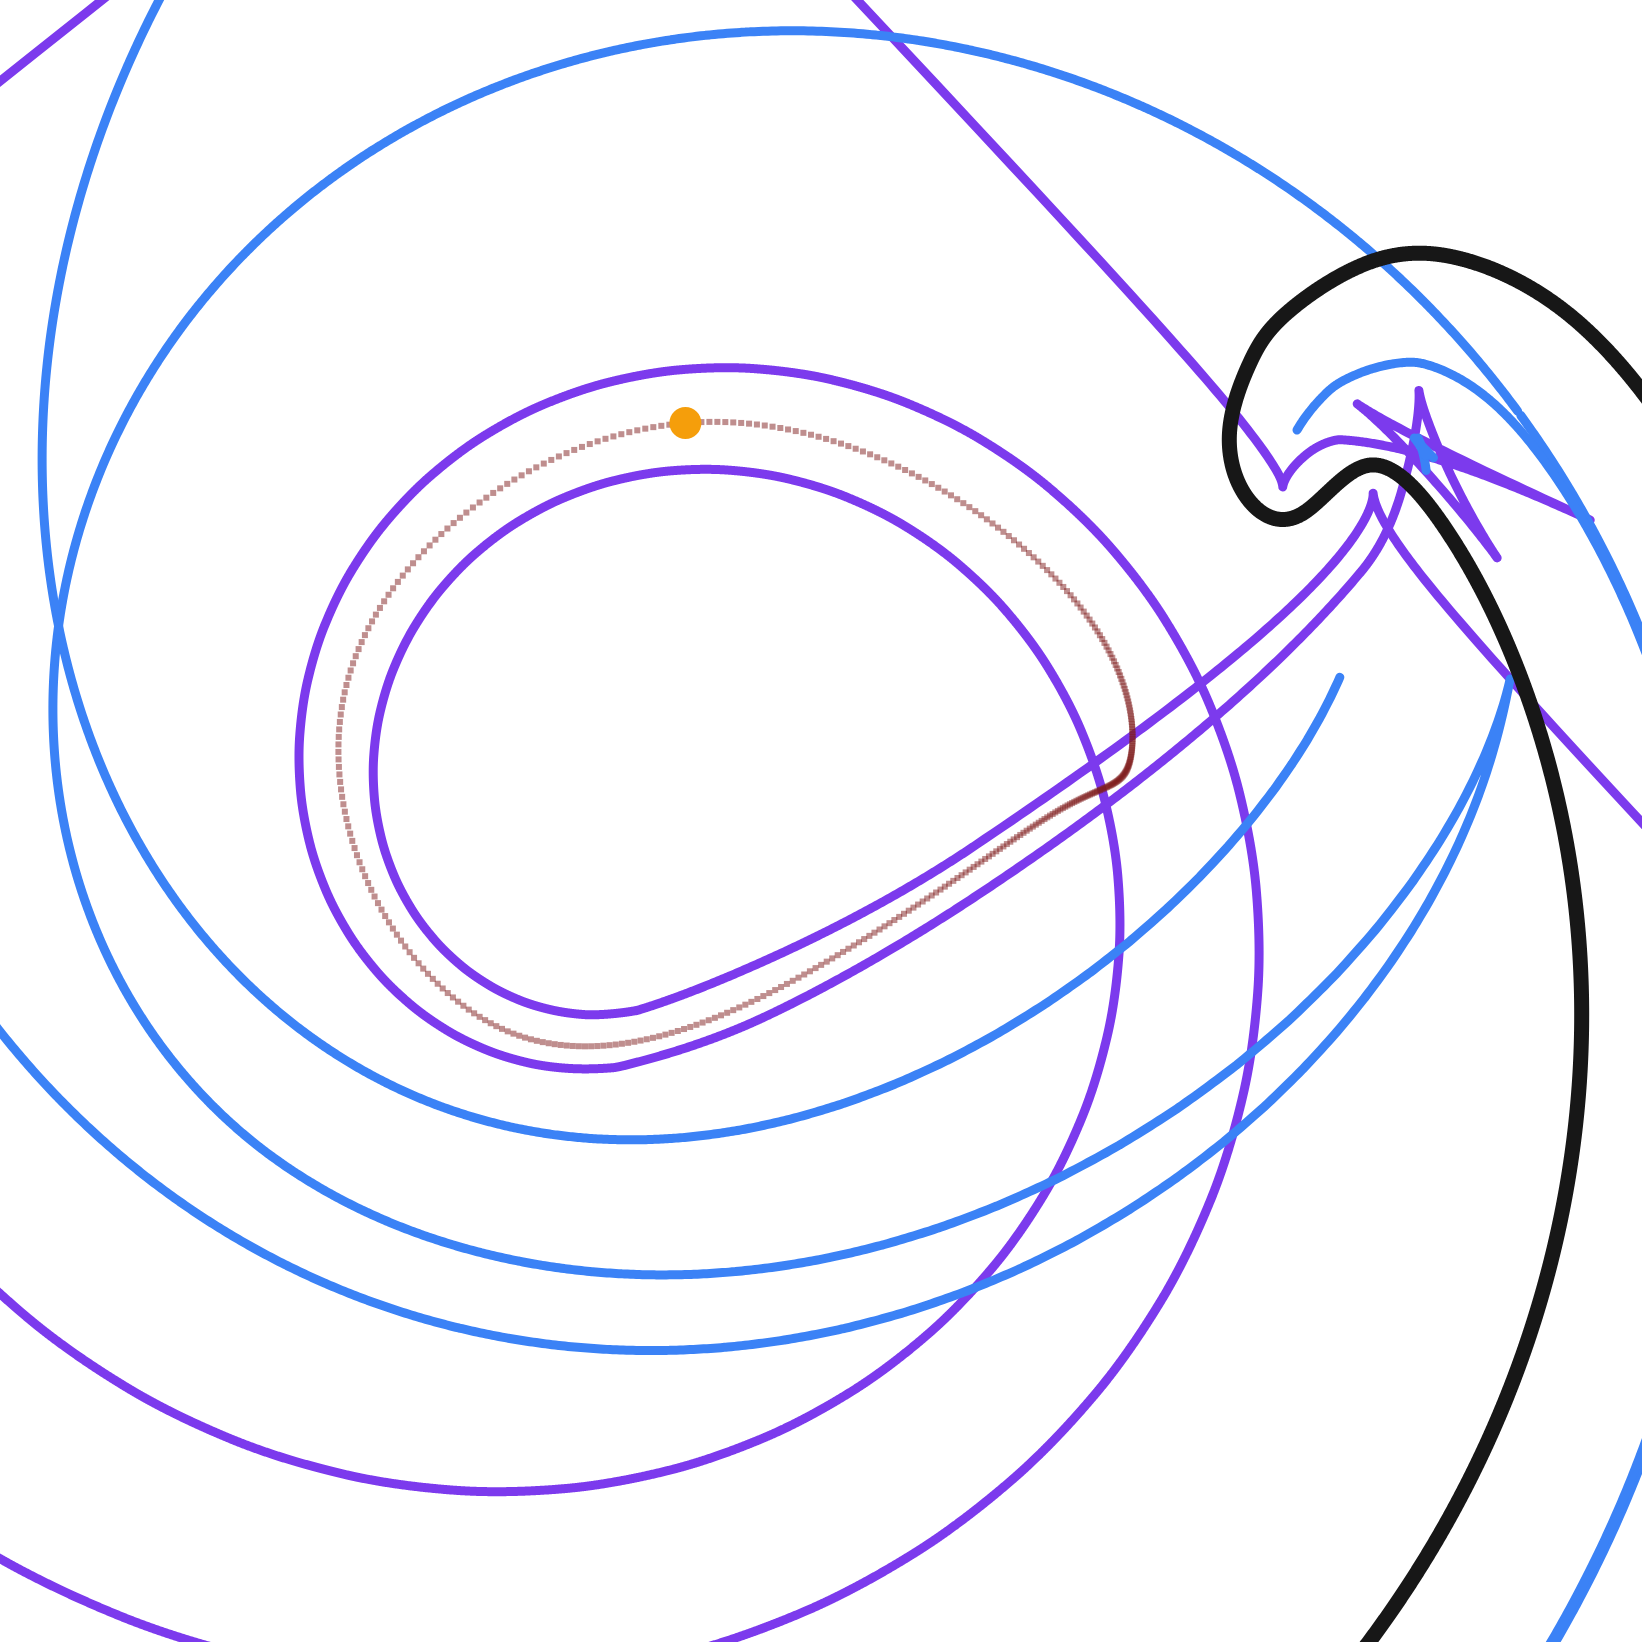
\includegraphics[width=0.3\linewidth]{figures/bishop_zoom.png}
    \hspace{0.5em}
    \fbox{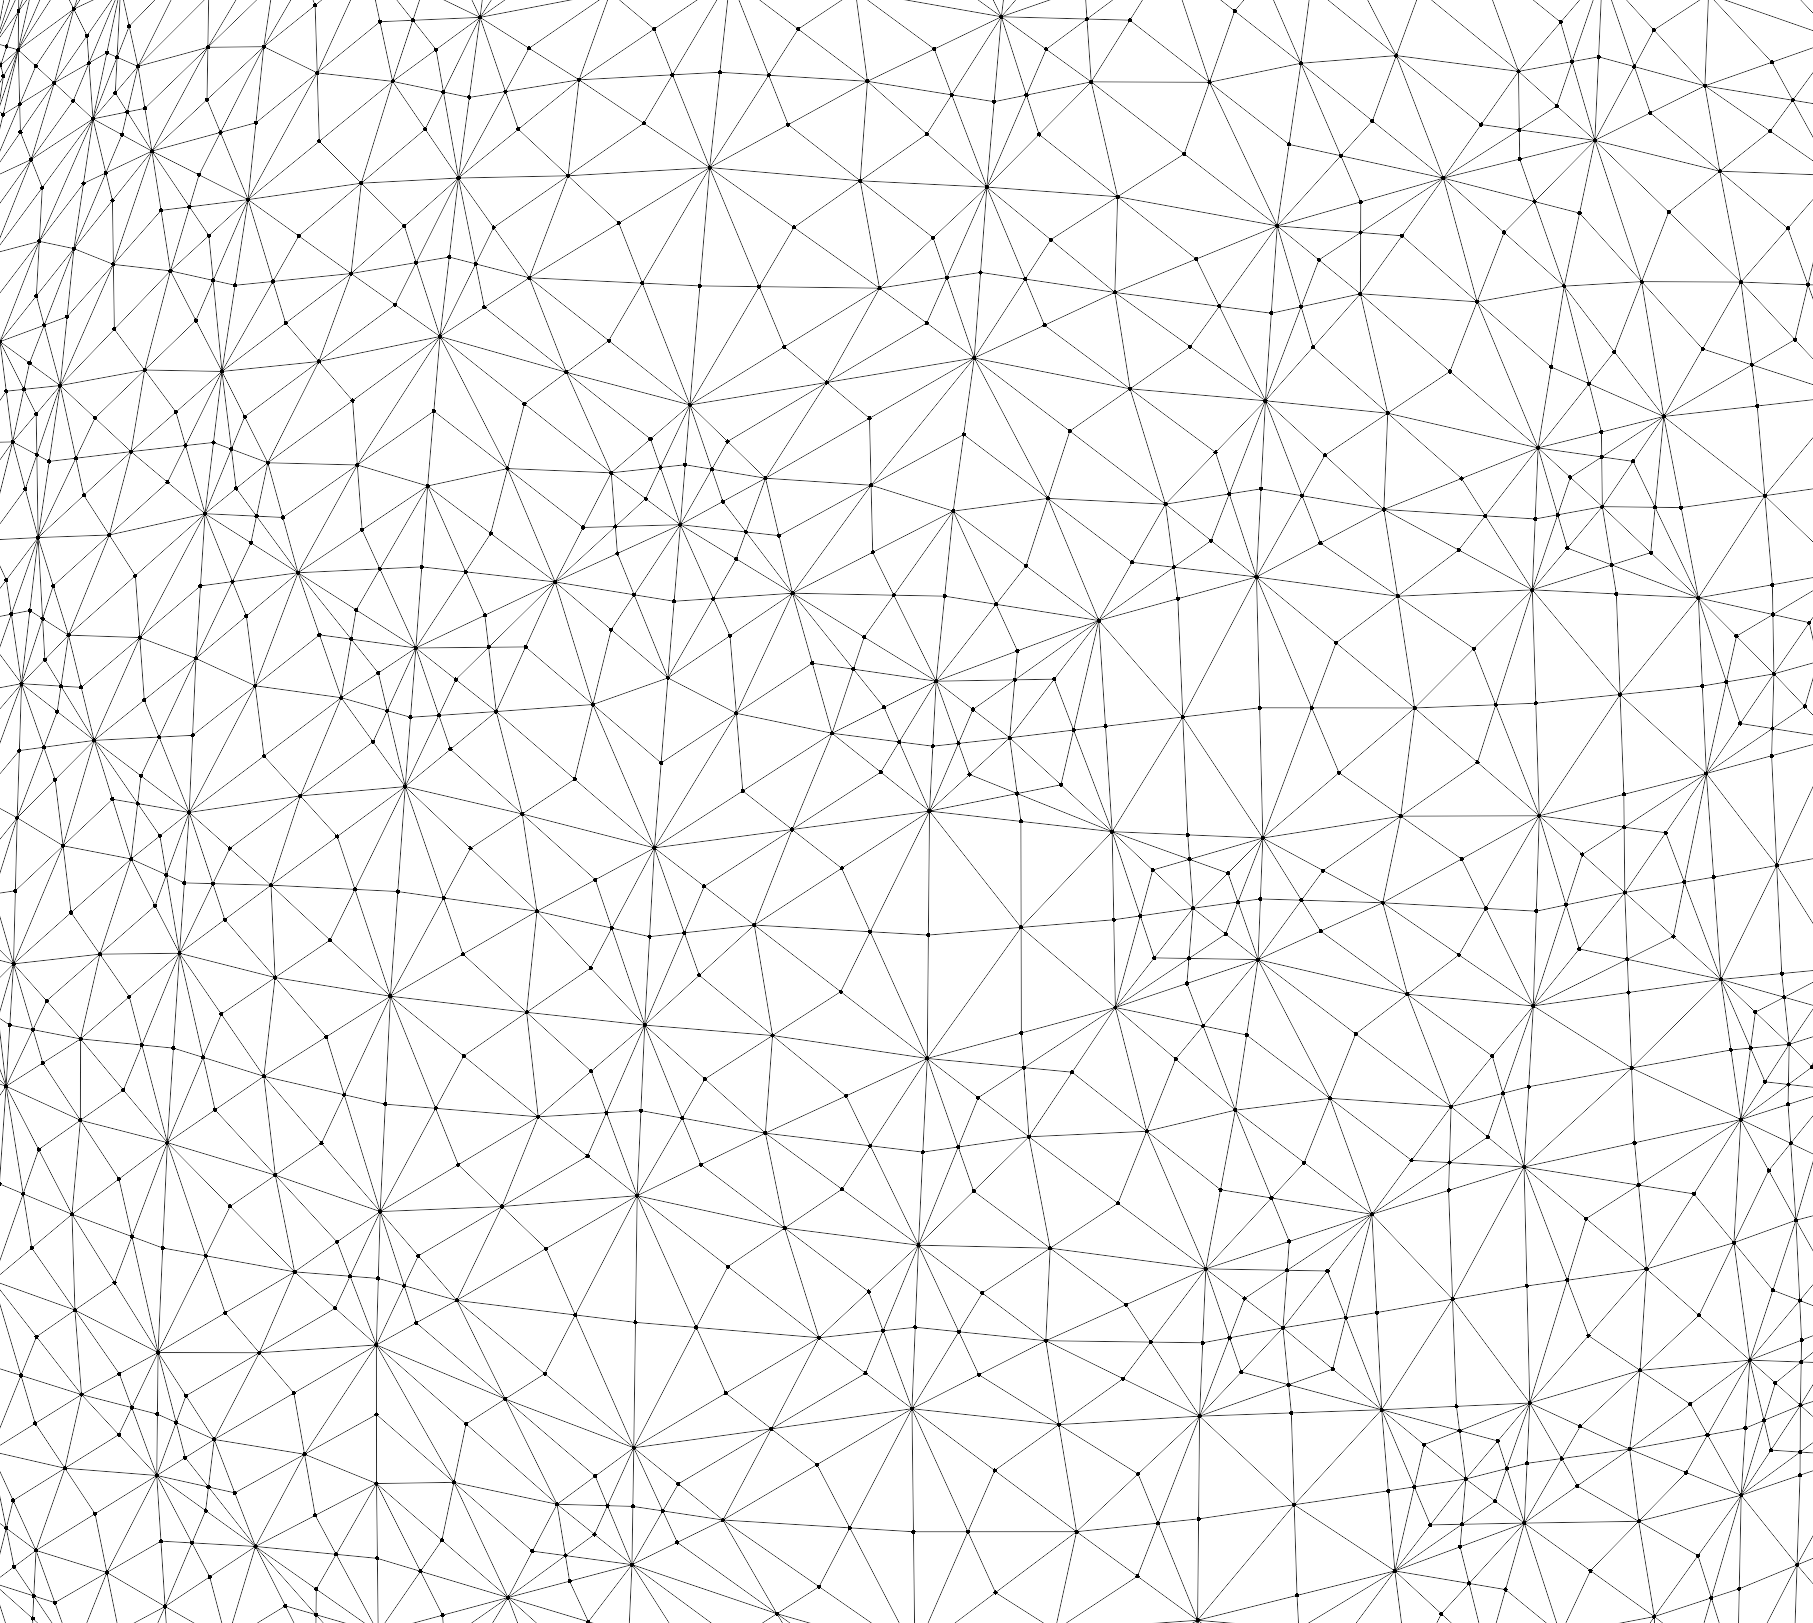
\includegraphics[width=0.35\linewidth]{torus_good.png}}
    % \caption{using constants closer to the paper (left) and with constants much farther away (right).}
    \label{fig:torus_triang}
\end{figure}
    
\end{frame}

\begin{frame}{Roadmap to stratified meshing}
    \begin{center}
        manifolds \;$\to$\; manifolds with boundary \;$\to$\; piecewise-smooth
        boundary \\[6pt] $\to$\; stratified spaces (strata meeting at nice angles)
        \\[6pt] $\to$\; finitely many singularity types (Thom / Arnold)
    \end{center}
    \vspace{0.8em}
    Manifold triangulation is the \textbf{first building block} of StratMesh's
    goal: certified meshes of stratified spaces.
    \note{The long-term arc tying the PhD to the grant. ~1 min.}
\end{frame}

%========================================================================
\section{Plan}
%========================================================================

\begin{frame}{Ongoing and future work}
    \begin{itemize}
        \item \textbf{Global monodromy criteria} \hfill{\footnotesize(short term)}\\
              {\footnotesize Extend the local analysis to loops of arbitrary size.}
        \item \textbf{Case analysis / higher-order medial axis}
              \hfill{\footnotesize(short term)}\\
              {\footnotesize Which branches near a singularity allow pairing
              changes --- a classification of $k$-th order medial-axis
              singularities.}
        \item \textbf{Higher dimensions} \hfill{\footnotesize(mid term)}\\
              {\footnotesize $\R^3$ and beyond, on the 3D symmetry-set
              classification.}
        \item \textbf{Stratified meshing} \hfill{\footnotesize(mid--long term)}\\
              {\footnotesize Certified meshes of stratified spaces under StratMesh.}
    \end{itemize}
    \note{Timeline for the committee: this year vs later. ~1.5 min.}
\end{frame}

\begin{frame}{Output so far}
    Two peer-reviewed workshop papers and one full preprint (all with Chambers,
    Fillmore, Mukherjee, Stephenson, Wintraecken):
    \begin{itemize}
        \item[{[P1]}] \emph{Bouquet: A Visualization Tool for Symmetry Sets and
              Vineyards.} EuroCG 2026.
        \item[{[P2]}] \emph{The symmetry set as a knitting pattern for vineyards.}
              CG:YRF 2026.
        \item[{[P3]}] \emph{The Singular Source of Vineyard Monodromy.} 2026,
              arXiv:2607.01046 (submitted to SODA).
    \end{itemize}
    \note{Quick -- they have the report. ~0.5 min.}
\end{frame}

% \section{References}
% \begin{frame}[allowframebreaks]{References}
% \footnotesize
%     \printbibliography
% \end{frame}

\begin{frame}[plain]
	\begin{center}
		{\Huge Thank You!}

		\bigskip\bigskip

		{\LARGE Questions?}

		\bigskip
		% {\footnotesize Bouquet2D: \url{https://bouquet2d.rohitroy.me}}
	\end{center}
\end{frame}

%----------------------------------------------------------------------------------------

\end{document}